%%%%%%%%%%%%%%%%%%%%%%%%%%%%%%%%%%%%%%%%%%  不使用 authblk 包制作标题  %%%%%%%%%%%%%%%%%%%%%%%%%%%%%%%%%%%%%%%%%%%%%%
%-------------------------------PPT Title-------------------------------------
\title{{\rm WIEN2k}软件:~基本理论与{\rm LAPW}方法}
%-----------------------------------------------------------------------------
%----------------------------Author & Date------------------------------------

%\author[\textrm{Jun\_Jiang}]{姜\;\;骏\inst{}} %[]{} (optional, use only with lots of authors)
%% - Give the names in the same order as the appear in the paper.
%% - Use the \inst{?} command only if the authors have different
%%   affiliation.
%\institute[BCC]{\inst{}%
\institute[Gain~Strong]{\inst{}%
%\vskip -20pt 北京市计算中心}
\vskip -20pt {\large 格致斯创(北京)科技有限公司}}
\date[\today] % (optional, should be abbreviation of conference name)
{%	{\fontsize{6.2pt}{4.2pt}\selectfont{\textcolor{blue}{E-mail:~}\url{jiangjun@bcc.ac.cn}}}
\vskip 45 pt {\fontsize{8.2pt}{6.2pt}\selectfont{北京%清华大学\;\;物理系% 报告地点
	\vskip 5 pt \textrm{2023.10.~21-23}}}
}

%% - Either use conference name or its abbreviation
%% - Not really information to the audience, more for people (including
%%   yourself) who are reading the slides onlin%%   yourself) who are reading the slides onlin%%   yourself) who are reading the slides onlineee

\subject{}
% This is only inserted into the PDF information catalog. Can be left
% out.
%\maketitle
\frame
{
%	\frametitle{\fontsize{9.5pt}{5.2pt}\selectfont{\textcolor{orange}{“高通量并发式材料计算算法与软件”年度检查}}}
\titlepage
}

%------------------------------------------------------------------------------列出全文 outline ---------------------------------------------------------------------------------
\section*{}
\frame[allowframebreaks]
{
  \frametitle{Outline}
%  \frametitle{\textcolor{mycolor}{\secname}}
  \tableofcontents%[current,currentsection,currentsubsection]
}
%在每个section之前列出全部Outline
%类似的在每个subsection之前列出全部Outline是\AtBeginSubsection[]
%\AtBeginSection[]
%{
%  \frame<handout:0>
%  {
%    \frametitle{Outline}
%全部Outline中,本部分加亮
%    \tableofcontents[current,currentsection]
%  }
%}

%------------------------------------------------------------------------------PPT main Body------------------------------------------------------------------------------------
\small
\frame
{
	\frametitle{材料计算软件发展现状}
\begin{figure}[h!]
\vspace*{-0.16in}
\centering

\includegraphics[width=3.30in]{Figures/Softwares_logo.png}
%\caption{\tiny \textrm{Pseudopotential for metallic sodium, based on the empty core model and screened by the Thomas-Fermi dielectric function.}}%(与文献\cite{EPJB33-47_2003}图1对比)
\label{Softwares}
\end{figure}
}

\frame
{
	\frametitle{国产第一原理计算软件现状}
\begin{figure}[h!]
\vspace*{-0.19in}
\centering
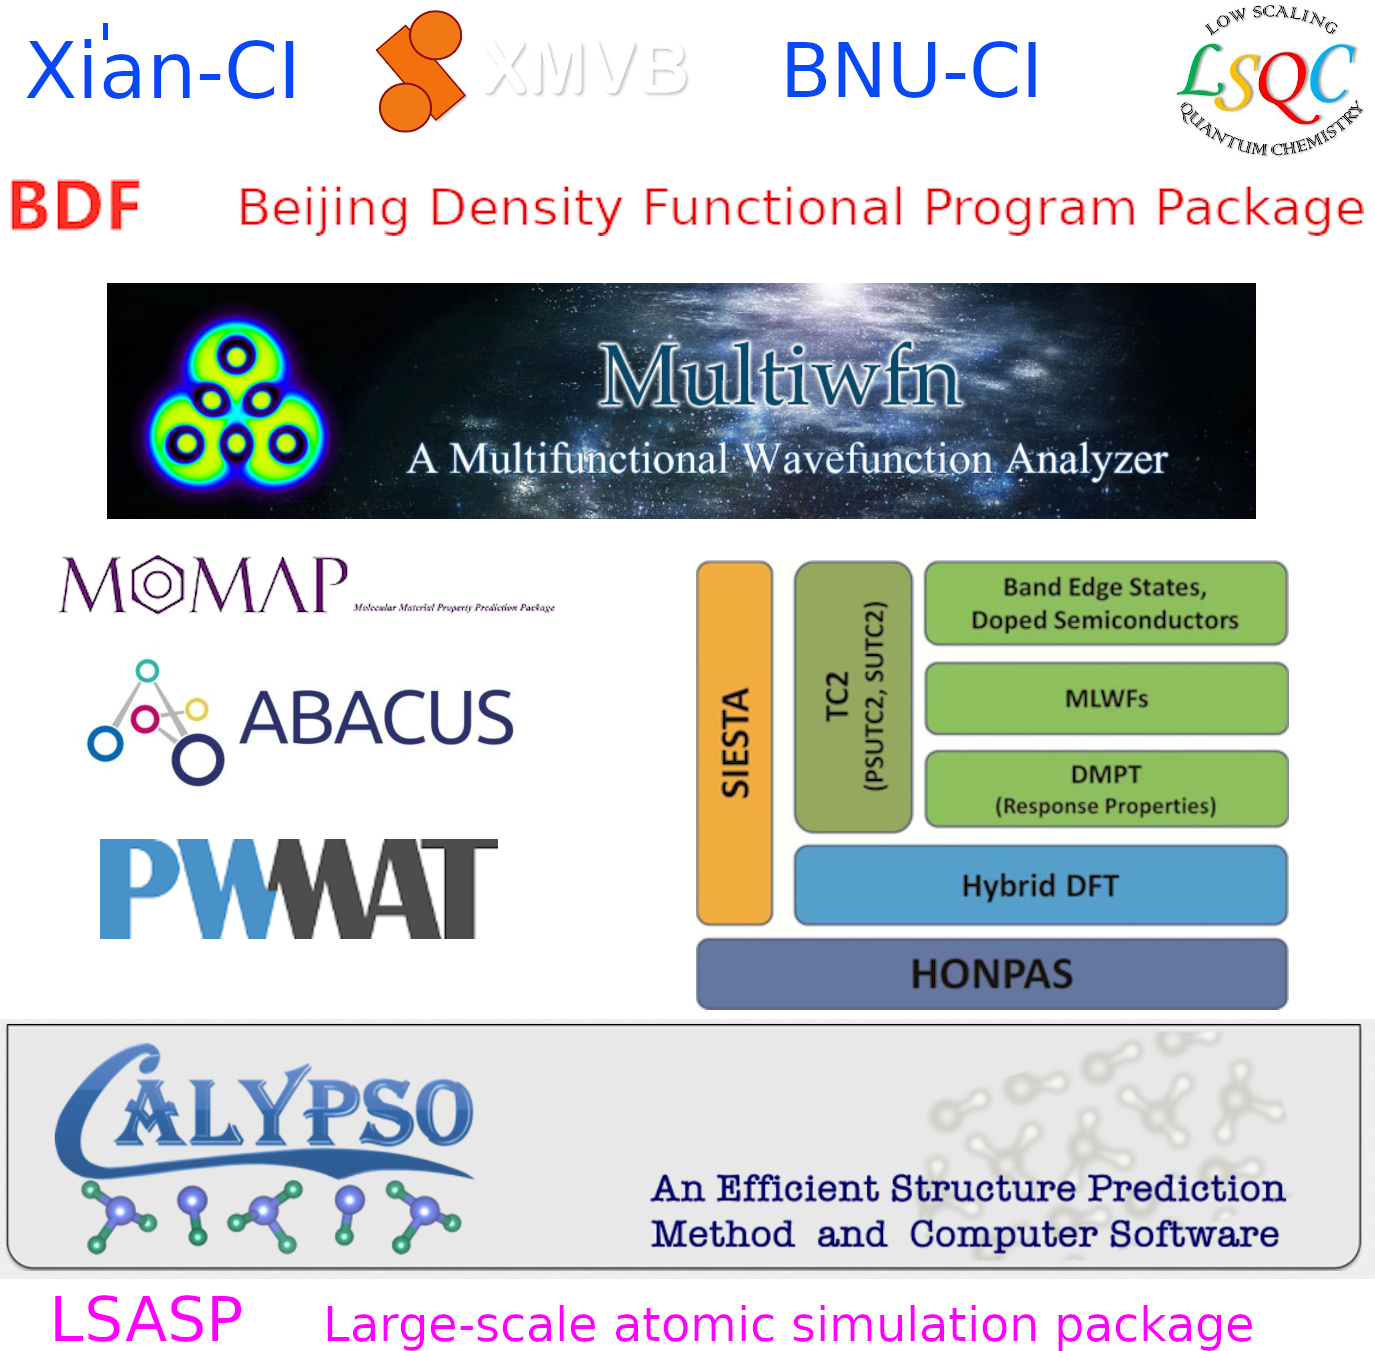
\includegraphics[width=2.83in]{Figures/Softwares_China-logo.png}
%\caption{\tiny \textrm{Pseudopotential for metallic sodium, based on the empty core model and screened by the Thomas-Fermi dielectric function.}}%(与文献\cite{EPJB33-47_2003}图1对比)
\label{Software-China}
\end{figure}
	\fontsize{6.2pt}{5.2pt}\selectfont{\textcolor{red}{中国学科发展战略\,$\cdot$\,理论与计算化学,~~国家自然科学基金委员会,~中国科学院,~~北京:~科学出版社,~~2016}}
}

\frame
{
\frametitle{\textrm{WIEN2k}软件简介}
\begin{figure}[h!]
\centering
\vspace*{-0.16in}
%\subfigure[\footnotesize{Logo of WIEN2k}]{
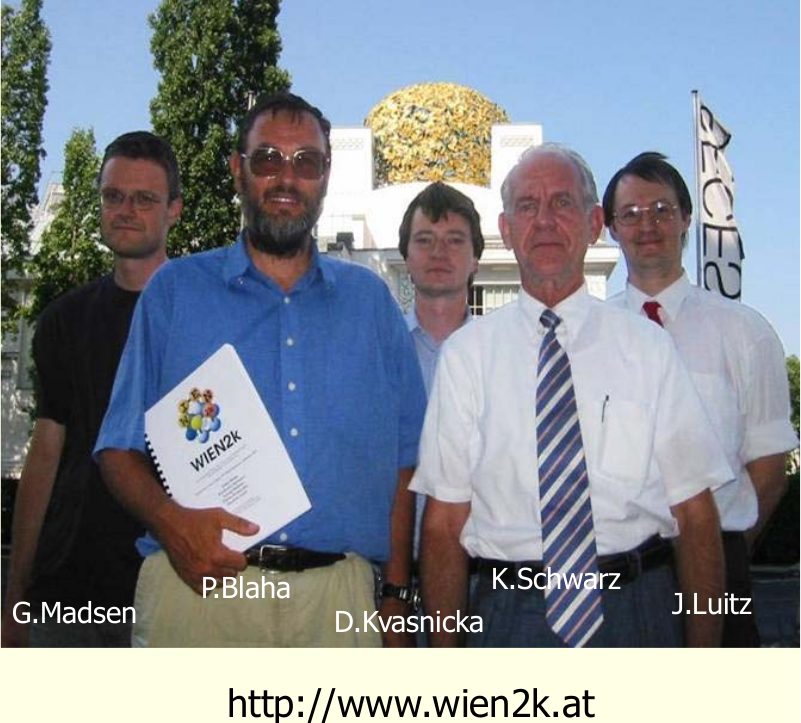
\includegraphics[height=1.5in]{Figures/WIEN2k-Group.png}
\hskip 0.5pt
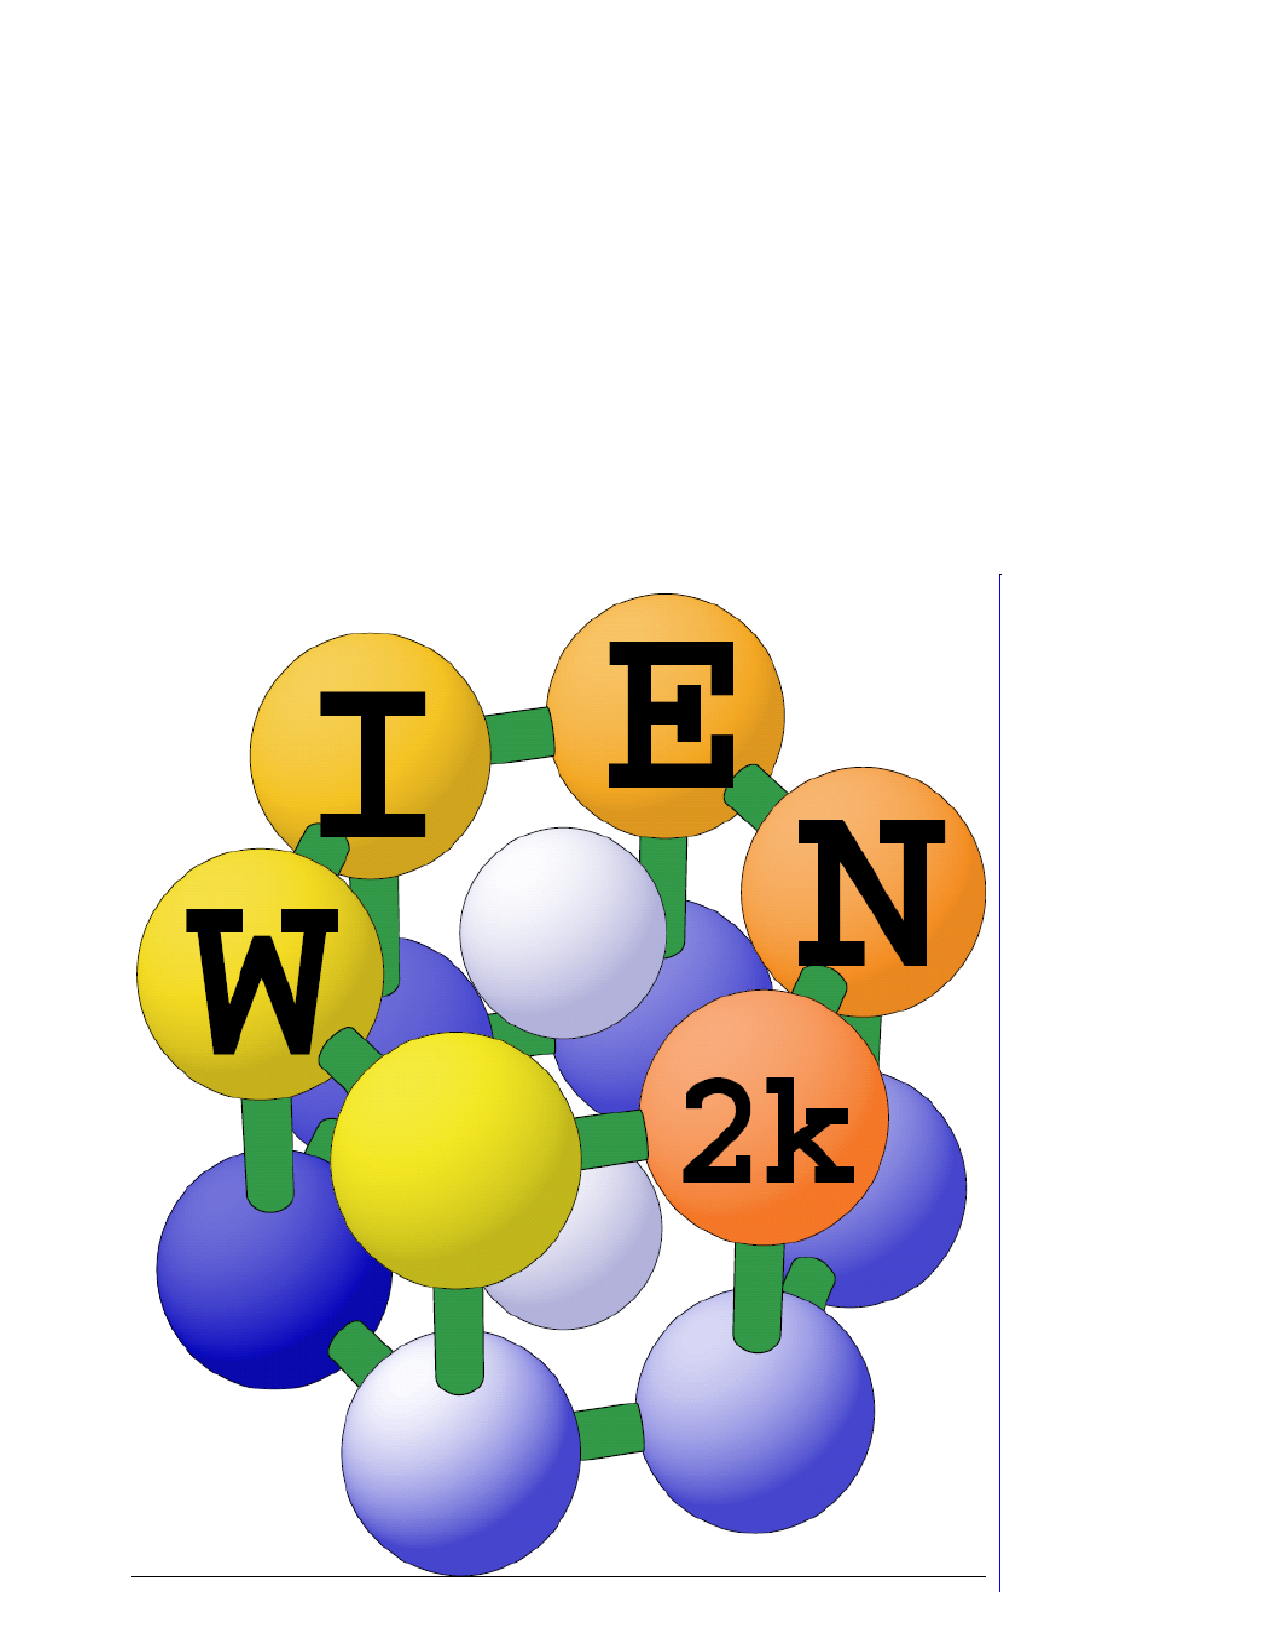
\includegraphics[height=1.5in,width=1.6in,viewport=13 35 475 515,clip]{Figures/logo_WIEN2k.pdf}
%\caption{\small \textrm{}}%(与文献\cite{EPJB33-47_2003}图1对比)
%\label{Brillouin_Cube}
%}
%\subfigure[\footnotesize{Logo of VASP}]{
%\includegraphics[height=1.48in,width=2.24in,viewport=55 145 595 455,clip]{logo_VASP.eps}
%\caption{\small \textrm{}}%(与文献\cite{EPJB33-47_2003}图1对比)
\label{Logo_of_WIEN2k}
%}
\end{figure}
\textrm{WIEN2k}是由奥地利维也纳技术大学\textrm{(Vienna University of Technology)}开发的高精度第一原理材料计算软件包\upcite{WIEN2k_UG}。%\\\textrm{WIEN2k};\textrm{VASP}。
\begin{itemize}
	\item 采用普适的全势\textrm{(Full-Potential, FP)}方法\\对计算对象的化学环境依赖小
	\item \textrm{LAPW}基组\\兼备描述波函数邻近原子核和位于原子核间行为的能力
	\item 计算精度高,结果常作为理论计算的\textrm{Benchmark}
%	\item \textrm{VASP}:采用\textrm{USPP-PAW}方法,计算效率高,特别擅长计算材料的力学性质\upcite{VASP_UG}
\end{itemize}
}

\frame
{
	\frametitle{\textrm{WIEN2k}软件简介}
\begin{minipage}[t]{0.55\textwidth}
	制约\textrm{WIEN2k}软件应用的主要因素
	\begin{itemize}
		\item 高精度计算必须付出的代价\\
			\textcolor{blue}{计算速度慢,处理体系有限}
		\item 各计算模块部分独立\\
			\textcolor{red}{输入控制文件过多}\\
			\textcolor{red}{输出数据文件分散}
		\item 采用\textrm{tcsh}脚本串联各部分\\
			计算中间结果需写入外部存储\\
			\textcolor{red}{\textrm{I/O}耗时过多}
		\item 软件的并行环境设置拙劣\\
			\textcolor{red}{\textrm{mpi}并行效率低下}
		\item \textcolor{red}{编译安装繁琐}
	\end{itemize}
\end{minipage}
\hfill
\begin{minipage}[t]{0.43\textwidth}
\begin{figure}[h!]
\centering
\vspace*{-10pt}
\includegraphics[height=2.6in,width=1.60in,viewport=60 90 325 500,clip]{Figures/WIEN2k_Program_flow.pdf}
\caption{\tiny \textrm{Program flow in WIEN2k.}}%(与文献\cite{EPJB33-47_2003}图1对比)
\label{WIEN2k_program_flow}
\end{figure}
\end{minipage}
}

\section{自由电子气与密度泛函理论}       %Bookmark
\frame
{
	\frametitle{\textrm{Thomas-Fermi}模型} 
	\textrm{1927}年,\textrm{Thomas}和\textrm{Fermi}基于均匀电子气模型上建立\textrm{Thomas-Fermi}模型,\textcolor{blue}{体系能量可用}\textcolor{red}{电子密度}\textcolor{blue}{表示}:
	\begin{itemize}
		\item 动能表达式
			$$T_{\mathrm{TF}}[\rho(\vec r)]=\dfrac3{10}(3\pi^2)^{\frac23}\int\rho^{\frac53}(\vec r)\mathrm{d}\vec r$$
		\item 外势$V_{ext}(\vec r)$下电子体系的能量泛函表达式为
			\begin{displaymath}
				\begin{aligned}
					E_{\mathrm{TF}}[\rho(\vec r)]=&\dfrac3{10}(3\pi^2)^{\frac23}\int\rho^{\frac53}(\vec r)\mathrm{d}\vec r\\
					&+\int\rho(\vec r)V_{ext}(\vec r)\mathrm{d}\vec r+\dfrac12\int\int\dfrac{\rho(\vec r_1)\rho(\vec r_2)}{|\vec r_2-\vec r_1|}\mathrm{d}\vec r_1\mathrm{d}\vec r_2
				\end{aligned}
			\end{displaymath}
		\item \textrm{Thomas-Fermi}模型完全没有考虑电子的交换-相关作用
	\end{itemize}
}

\frame
{
	\frametitle{\textrm{Thomas-Fermi-Dirac}模型} 
	1930年,\textrm{Dirac}将\textrm{Thomas-Fermi}模型修正,用局域密度近似考虑电子交换作用
			\begin{displaymath}
				\begin{aligned}
					E_{\mathrm{TFD}}[\rho(\vec r)]=&\dfrac3{10}(3\pi^2)^{\frac23}\int\rho^{\frac53}(\vec r)\mathrm{d}\vec r+\int\rho(\vec r)V_{ext}(\vec r)\mathrm{d}\vec r\\
					&+\dfrac12\int\int\dfrac{\rho(\vec r_1)\rho(\vec r_2)}{|\vec r_2-\vec r_1|}\mathrm{d}\vec r_1\mathrm{d}\vec r_2-\dfrac34\bigg(\dfrac3{\pi}\bigg)^{\frac13}\int\rho^{\frac43}(\vec r)\mathrm{d}\vec r
				\end{aligned}
			\end{displaymath}
			\begin{itemize}
				\item 在总电子数守恒约束条件
					$$\int\rho(\vec r)\mathrm{d}\vec r=N$$
					下,能量泛函$E_{\mathrm{TFD}}[\rho(\vec r)]$对密度$\rho(\vec r)$的变分极小获得体系的基态密度和基态能量
			\end{itemize}
}

\frame
{
	\frametitle{\textrm{Thomas-Fermi}模型}
	\begin{itemize}
		\item \textrm{Thomas-Fermi}模型用电子密度代替波函数描述问题是极大的简化,但模型过于粗糙:\\
%			\begin{enumerate}
%				\item 以均匀电子气的密度得到动能的表达式
%				\item 完全忽略电子间的交换-相关作用
%			\end{enumerate}
			不能正确描述相互作用电子体系的基本特征,如原子的壳层结构
		\item \textrm{Thomas-Fermi}模型虽不够精确,但可以通过引入修正项校正:
			\textrm{Dirac}交换泛函 $$E_X[\rho(\vec r)]=-\dfrac34\bigg(\dfrac3{\pi}\bigg)^{\frac13}\int\rho^{\frac43}(\vec r)\mathrm{d}\vec r$$
			\textrm{Wigner}相关泛函 $$E_C[\rho(\vec r)]=-0.056\int\dfrac{\rho^{\frac43}(\vec r)}{0.079+\rho^{\frac13}(\vec r)}\mathrm{d}\vec r$$
	\end{itemize}
	\textrm{Thomas-Fermi}模型为密度泛函理论\textrm{(DFT)}提供了重要的启示
}

\frame                               %
{
\frametitle{密度泛函理论(\textrm{DFT})} %Slide Page Title
%   \secname
与传统的量子力学方法不同,密度泛函理论的基本变量是体系的基态电子密度。%通过体系的电子密度而非波函数确定体系的基态能量。
\begin{itemize}%[+-| alert@+>]
	\item 密度泛函理论的基石:\textrm{Hohenberg-Kohn}定理\upcite{PR136-B864_1964}
\vskip 5pt
\begin{itemize}%[+-| alert@+>]
   \setlength{\itemsep}{8pt}
 \item $E[\rho]=F_{\mathrm{HK}}[\rho]+\displaystyle\int\rho(\vec{r})v(\vec{r})\textrm{d}\vec{r}$ \\
\vskip 5pt 
{\fontsize{7.2pt}{6.2pt}\selectfont{其中$F_{\mathrm{HK}}[\rho]=\underset{\Psi\to\rho}{\mathrm{Min}}\langle\Psi[\rho]|\hat{T}+\hat{W}|\Psi[\rho]\rangle$
是普适的泛函表达式。}}\\%,指明多电子体系的基态性质与基态密度间存在一一对应关系
\textcolor{magenta}{\fontsize{8.2pt}{6.2pt}\selectfont{第一定理表明多电子体系的性质完全由体系的基态密度决定}}
   \item 如果$\tilde\Psi\neq\Psi$,
     $E[\tilde\rho]\geqslant E[\rho_0]$\\
     \textcolor{magenta}{\fontsize{8.2pt}{6.2pt}\selectfont{第二定理指出基态总能量泛函在体系基态电子密度处取极小值}}
   \end{itemize}
\vskip 8pt
 \item 密度泛函理论的优越性:~用密度($\rho$)代替波函数($\Psi$)描述体系
\vskip 5pt
 \item 密度泛函理论的困难:~能量密度泛函的精确形式未知
   \end{itemize}
}

\frame                               %
{
\frametitle{密度泛函理论(\textrm{DFT})}
\textrm{Kohn-Sham}方程\upcite{PR140-A1133_1965}:无相互作用体系+交换-相关能的贡献
$$(T_S+V_{e\!f\!f})|\varphi_i\rangle=\varepsilon_i|\varphi_i\rangle,\quad i=1,\cdots,N,\cdots$$
其中$T_S=-\dfrac12\nabla^2$~~是无相互作用体系的动能
\begin{displaymath}
	\begin{aligned}
		V_{e\!f\!f}(\vec r)=&V_{ext}(\vec r)+\displaystyle\int w(\vec r,\vec r\,')\rho(\vec r\,')\mathrm{d}\vec r\,'+V_{\mathrm{XC}}[\rho]\\
=&\displaystyle\int\dfrac{\rho(\vec r\,')}{|\vec r-\vec r^{\prime}|}\mathrm{d}\vec r\,'+V_{ext}(\vec r)+V_{\mathrm{XC}}[\rho]
	\end{aligned}
\end{displaymath}
$V_{ext}(\vec r)$是电子体系与外部的电荷或磁场相互作用\\
$V_{\mathrm{XC}}[\rho]=\dfrac{\delta E_{\mathrm{XC}}}{\delta\rho(\vec r)}$称为交换-相关势
\vskip 10pt
\textrm{Kohn-Sham}方程是形式上的单粒子方程
\vskip 6pt
\textrm{Kohn-Sham}方程的实质:\\\textcolor{red}{将动能泛函的主要部分分离出来,剩余部分放在交换-相关能中}
}

\frame
{
\frametitle{交换-相关能与交换-相关势}
实际考虑交换-相关能时,会将交换-相关能表示为交换能和相关能之和:
\begin{displaymath}
	E_{\mathrm{XC}}[\rho]=E_{\mathrm{X}}[\rho]+E_{\mathrm{C}}[\rho]=\int\varepsilon_{\mathrm{X}}[\rho]\rho(\vec{r}) \textrm{d}^3\vec{r}+\int\varepsilon_{\mathrm{C}}[\rho]\rho(\vec{r}) \textrm{d}^3\vec{r}
\end{displaymath}
$\varepsilon_{\mathrm{X}}[\rho]$和$\varepsilon_{\mathrm{C}}[\rho]$可理解为单电子的交换能和相关能
\vskip 20pt
交换-相关势通过交换-相关能计算得到:~
		\begin{displaymath}
			V_{\mathrm{XC}}^{\sigma}[\rho_{\alpha},\rho_{\beta}]=\dfrac{\delta E_{\mathrm{XC}}[\rho_{\alpha},\rho_{\beta}]}{\delta\rho_{\sigma}}=\dfrac{\delta\{E_{\mathrm{X}}[\rho_{\alpha},\rho_{\beta}]+E_{\mathrm{C}}[\rho_{\alpha},\rho_{\beta}]\}}{\delta\rho_{\sigma}}
		\end{displaymath}
		\textcolor{red}{注意}:~由于$E_{\mathrm{XC}}[\rho_{\sigma}]$对$\rho_{\sigma}$是非线性的
		\vskip 8pt
		\textcolor{blue}{$V_{\mathrm{XC}}=V_{\mathrm{X}}+V_{\mathrm{C}}$和$\varepsilon_{\mathrm{XC}}=\varepsilon_{\mathrm{X}}+\varepsilon_{\mathrm{C}}$不同},\underline{\textcolor{purple}{不要混淆这两个量}}
}
%  \beamertemplateshadingbackground{blue!10}{yellow!10}

\frame                               %
{
\frametitle{交换-相关能密度泛函}
\textcolor{blue}{密度泛函理论的核心问题}:\\
\textrm{Kohn-Sham}方程用于实际计算,必须知道$E_{XC}[\rho]$或者$V_{XC}[\rho]$与$\rho(\vec r)$的泛函关系
\vskip 5pt
\begin{minipage}[b]{0.59\textwidth}
 \hspace*{-20pt}
 \vskip -55pt
 \fontsize{7.5pt}{6.0pt}\selectfont{
 \begin{itemize}%[+-| alert@+>]
	 \setlength{\itemsep}{10pt}
 \item \textrm{LDA}:泛函只与密度分布的局域值有关
 \item \textrm{GGA}:泛函依赖:局域密度及其梯度
 \item $meta$-\textrm{GGA}:泛函依赖的变量还有动能密度
 \item 杂化(\textrm{hybrid})泛函:泛函与占据轨道有关
 \item 其他的交换-相关能泛函
 \item<1-> 完全非局域泛函:理想泛函,不现实
 \end{itemize}
}
\end{minipage}
\hfill
\begin{minipage}[b]{0.39\textwidth}
\begin{figure}[h!]
\centering
\hspace*{-15pt}
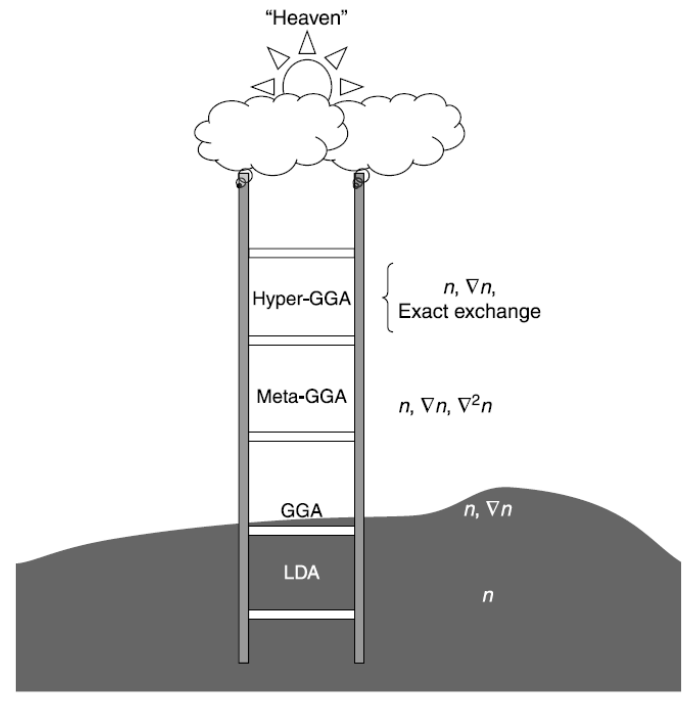
\includegraphics[height=1.7in,width=3.18in,viewport=10 5 1380 700,clip]{Figures/Jacobi-ladder.png}\\
%\caption{\tiny \textrm{}}%(与文献\cite{EPJB33-47_2003}图1对比)
\label{Jacob's_ladder}
\end{figure}
\vskip -10pt
\centering{\textcolor{red}{\textrm{\tiny Jacob's ladder}}}
\end{minipage}
% \begin{itemize}%[+-| alert@+>]
%\item 交换-相关能密度泛函
}

\frame                               %
{
	\frametitle{近似能量泛函$E_{\mathrm{XC}}[\rho]$的主要问题}
\vskip 20pt
\begin{enumerate}%[+-| alert@+>]
   \setlength{\itemsep}{10pt}
 \item  密度是整体变量:~电子自相互作用抵消不净\\%\quad\textrm{(LDA+U)}方法的校正%(\textrm{LDA+U})
	 用\textrm{DFT}计算电子数很少的体系,一般都会有较大的误差
 \item  电子相关:~简并和近简并基态的表示不合理\\
	 基态电子密度用不同的简并轨道计算时,体系能量应保持不变,但现有的近似能量泛函不具有这个性质
 \item  渐近行为:~处理弱相互作用体系的误差大\\
	 如\textrm{Van der Waals}相互作用和现有近似能量泛函本身的计算误差在同一量级
 \end{enumerate}
}

\frame                               %
{
	\frametitle{\textrm{Kohn-Sham}方程}
\begin{figure}[h!]
\centering
\vspace*{-0.21in}
\hspace*{-0.1in}
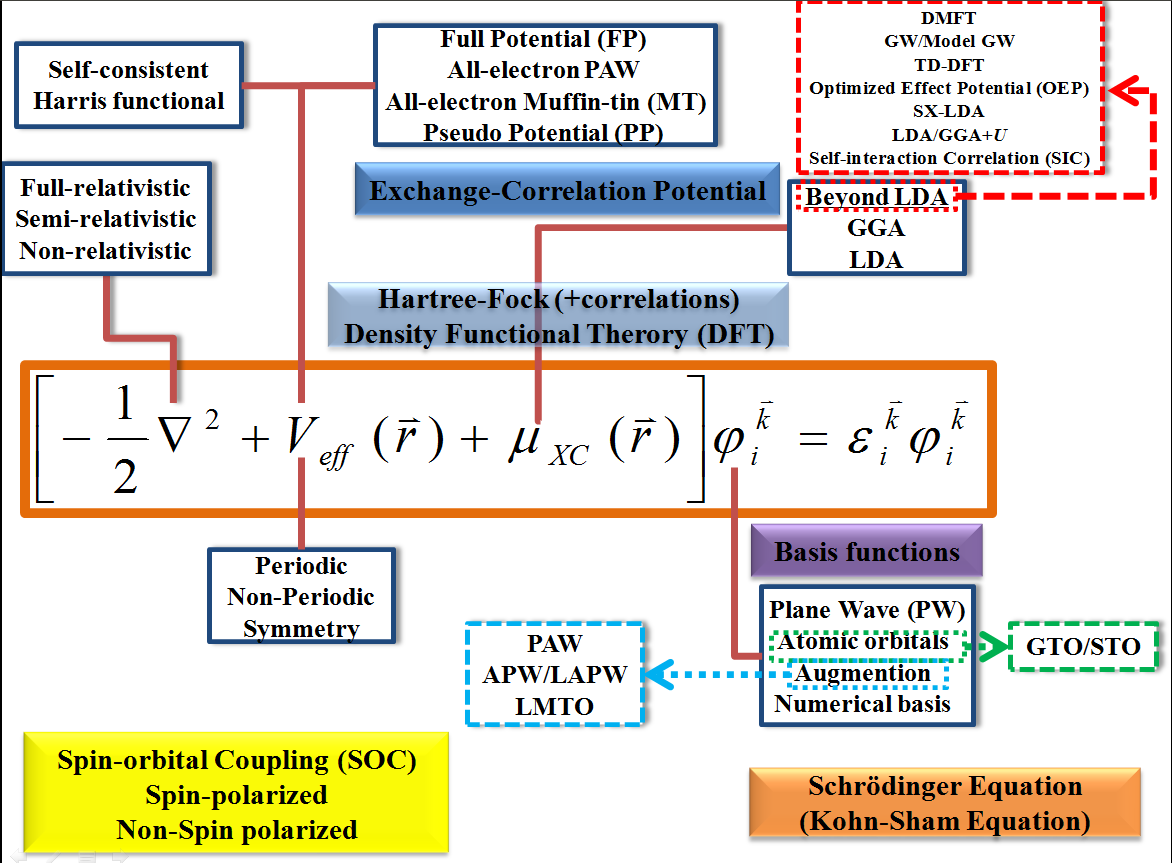
\includegraphics[height=2.7in,width=4.0in,viewport=2 5 1162 880,clip]{Figures/DFT.png}
\caption{\tiny \textrm{The Analysis of Kohn-Sham equation.}}%(与文献\cite{EPJB33-47_2003}图1对比)
\label{DFT}
\end{figure}
}

\frame
{
	\frametitle{\textrm{DFT-SCF}}
\begin{figure}[h!]
\centering
\vspace*{-0.25in}
\hspace*{-0.80in}
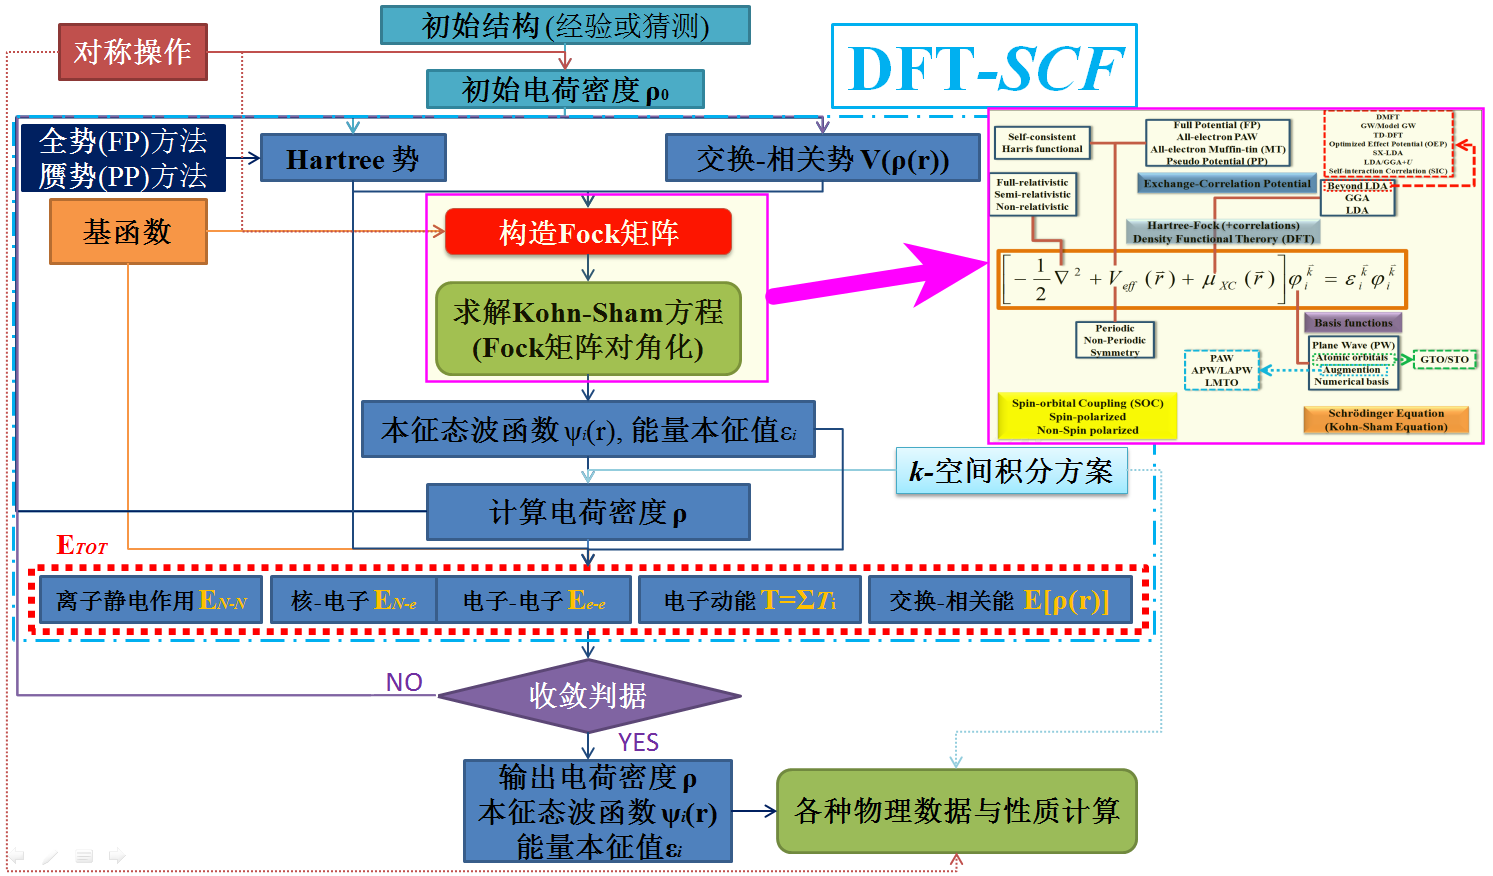
\includegraphics[height=2.80in,width=4.95in,viewport=5 3 1490 870,clip]{Figures/DFT-SCF_2.png}
%\caption{\tiny \textrm{Pseudopotential for metallic sodium, based on the empty core model and screened by the Thomas-Fermi dielectric function.}}%(与文献\cite{EPJB33-47_2003}图1对比)
\label{DFT-SCF-2}
\end{figure}
}

%\section{Induction on DFT and solid-state physics}       %Bookmark
\section{固体能带与赝势}       %Bookmark
\frame
{
%\frametitle{The Bloch theorem}
\frametitle{固体能带理论}
\begin{itemize}%[+-| alert@+>]
   \setlength{\itemsep}{8pt}
   \item 固体能带理论\upcite{Huang_Han}是固体电子理论的基础,形式上是\\单电子理论:
    $$\hat H |\psi_i^{\vec k}(\vec r)\rangle=\bigg[-\dfrac{\hbar^2}{2m}\nabla^2+V(\vec r)\bigg]|\psi_i^{\vec k}(\vec r)\rangle=\epsilon_i(\vec k)|\psi_i^{\vec k}(\vec r)\rangle$$
  \item \textrm{Bloch}定理:
%   \item \textrm{periodic potential:} $$V(\vec r)=V(\vec r+\vec R_n)$$
%     \textrm{Here,} $\vec R_n=n\vec R$
%   \item \textrm{Bloch theorem:}$$\psi_{\vec k}(\vec r)=\textrm{e}^{\textrm i\vec k\cdot\vec r}u_{\vec k}(\vec r)$$
%     \textrm{Here, $u_{\vec k}(\vec r)$ is a periodic function with the same periodicity as $V(\vec r)$, i.e., $u_{\vec k}(\vec r)=u_{\vec k}(\vec r+\vec R_n)$, then Bloch theorem could reads as:}
%     $$\psi_{\vec k}(\vec r+\vec R_n)=\textrm{e}^{\textrm i\vec k\cdot\vec R_n}\psi_{\vec k}(\vec r)$$
具有平移周期性的理想晶体,势能$V(\vec r)$满足$$V(\vec r)=V(\vec r+\vec R_n)$$
体系的波函数满足\textrm{Bloch}波函数形式:$$\psi_{\vec k}(\vec r)=\textrm{e}^{i\vec k\cdot\vec r}u_{\vec k}(\vec r)$$
是平面波和周期函数的乘积。$u(\vec r)$与势能有相同的周期。即$$u_{\vec k}(\vec r)=u_{\vec k}(\vec r+\vec R_n)$$
  \item 能带理论相当于分子轨道理论
%   \setlength{\itemsep}{30pt}
\item \textrm{Bloch}函数反映了波函数在周期性势场下的变化规律。
\end{itemize}
}

\frame
{
\frametitle{固体能带理论}
简并态微扰理论引起的能带裂分
\begin{figure}[h!]
\centering
%\hspace*{-10pt}
%\vspace*{-1.1in}
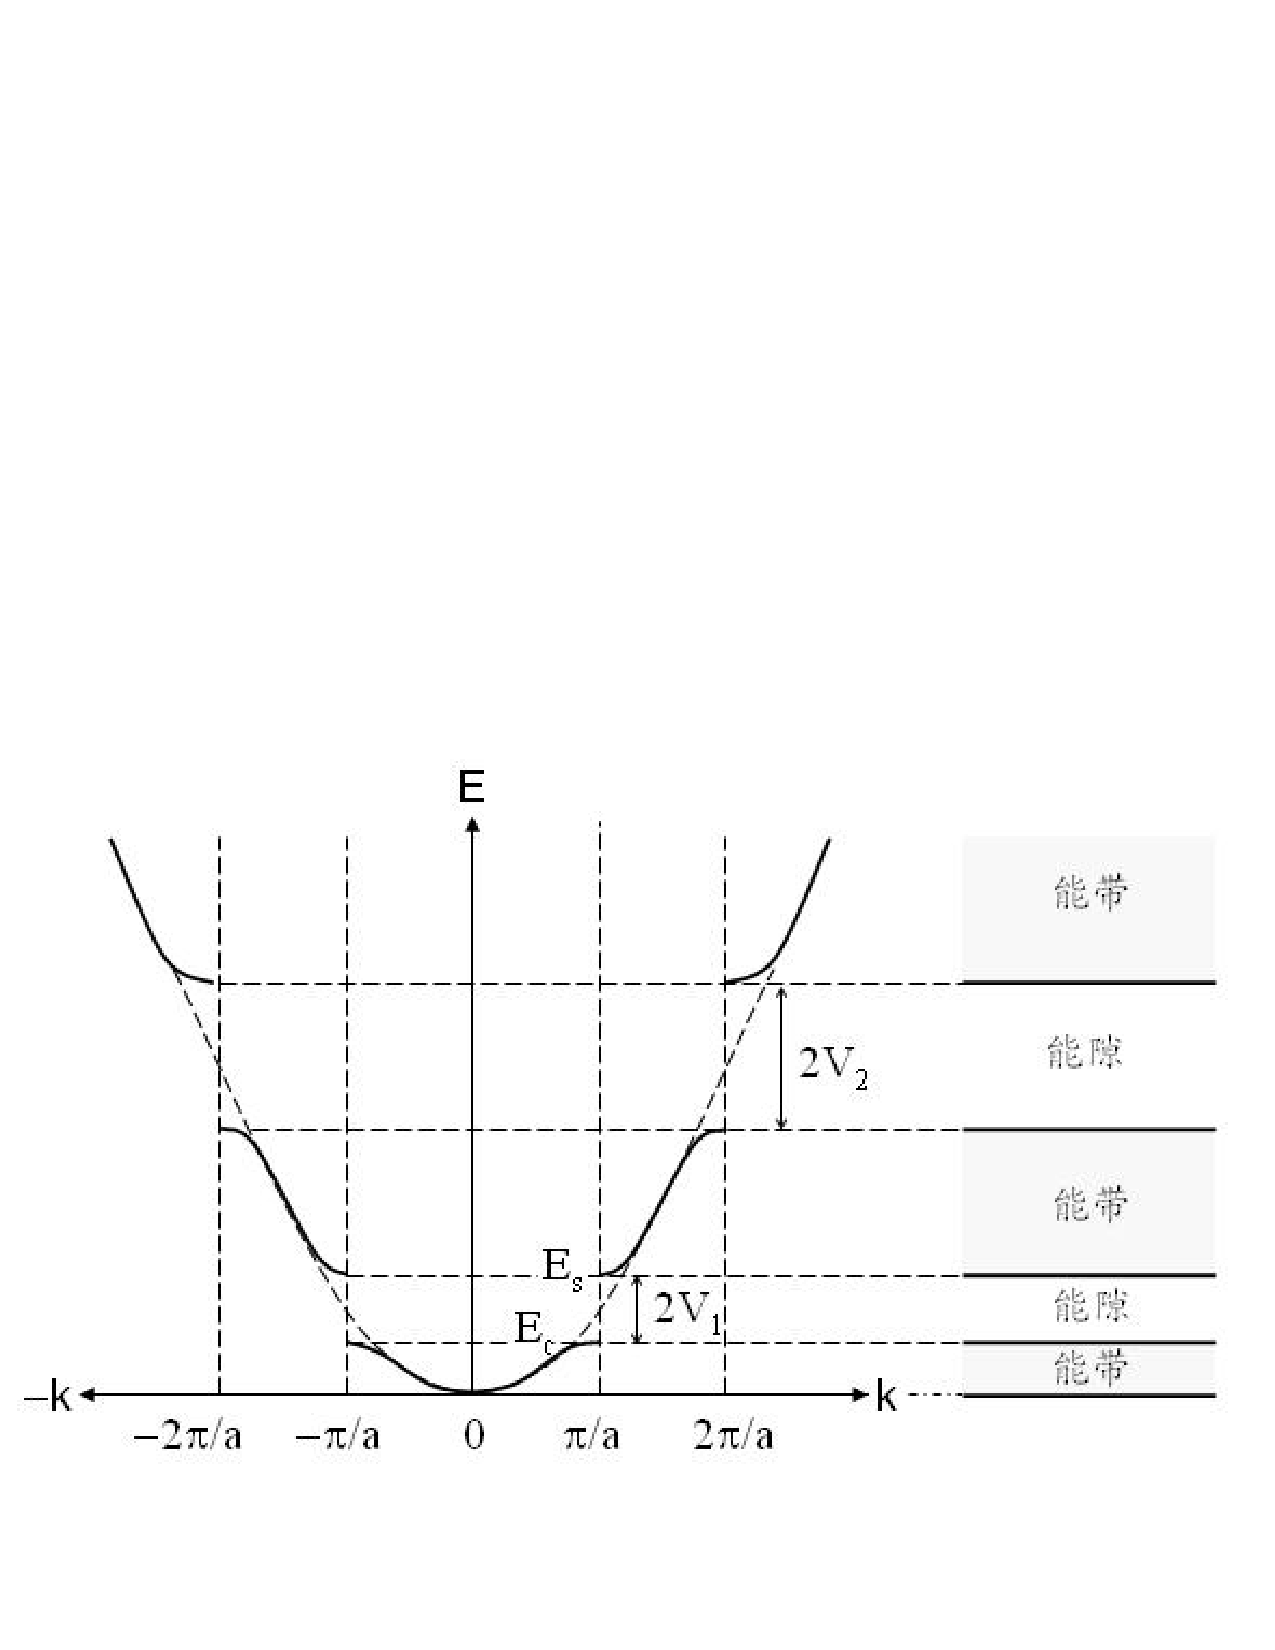
\includegraphics[height=2.1in,width=3.8in,viewport=10 90 570 380,clip]{Figures/Band_Gap.pdf}
\caption{\small \textrm{The Band-structure from free-electron gas.}}%
\label{Band-Structure-1}
\end{figure} 
}

\frame
{
\frametitle{固体能带理论}
从分子轨道到能带
\begin{figure}[h!]
\centering
\hspace*{-0.29in}
\vspace*{-0.1in}
\subfigure[一维$\mathrm{H}$原子链]{
\label{fig:Hydrogen-1D}
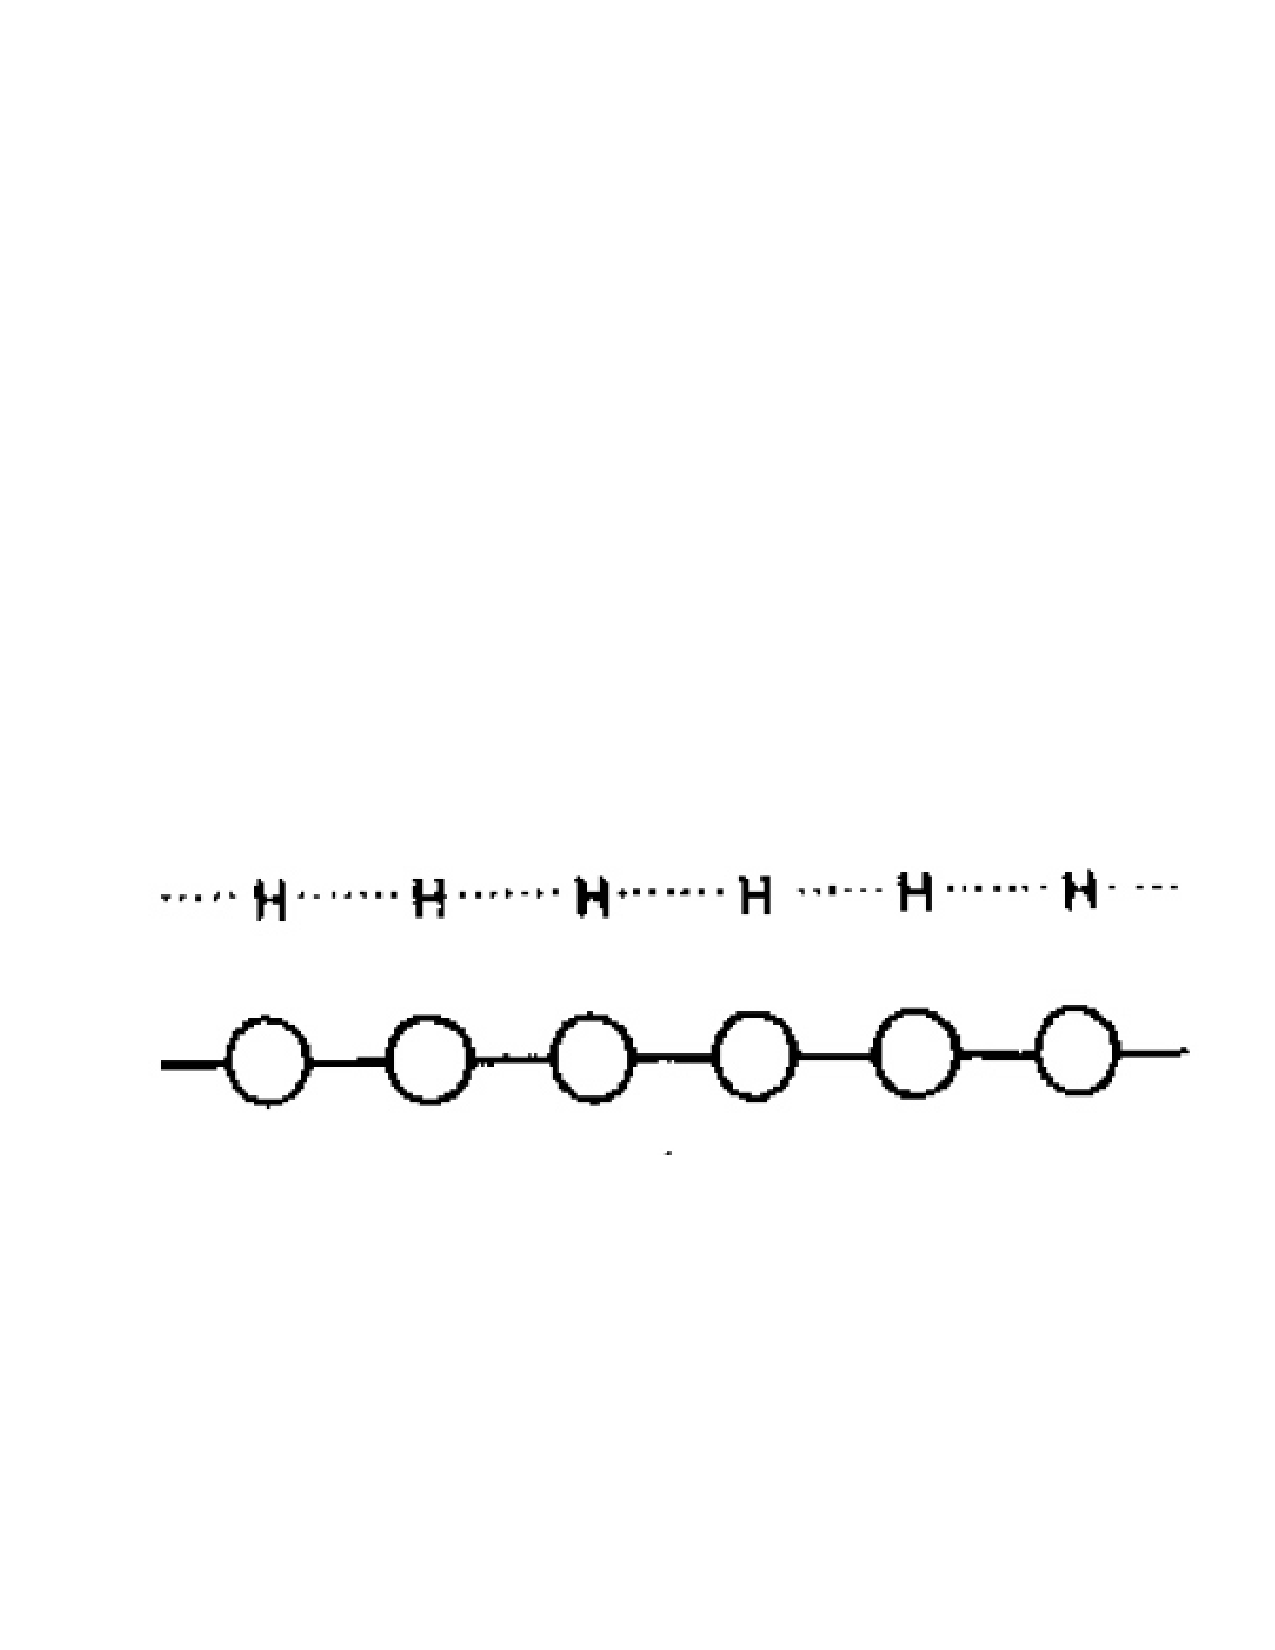
\includegraphics[height=0.25in,width=1.1in,viewport=70 255 570 375,clip]{Figures/Hydrogen-1D.pdf}}
\subfigure[$\mathrm{H}_n$分子轨道]{
\label{fig:Hydrogen-2-n}
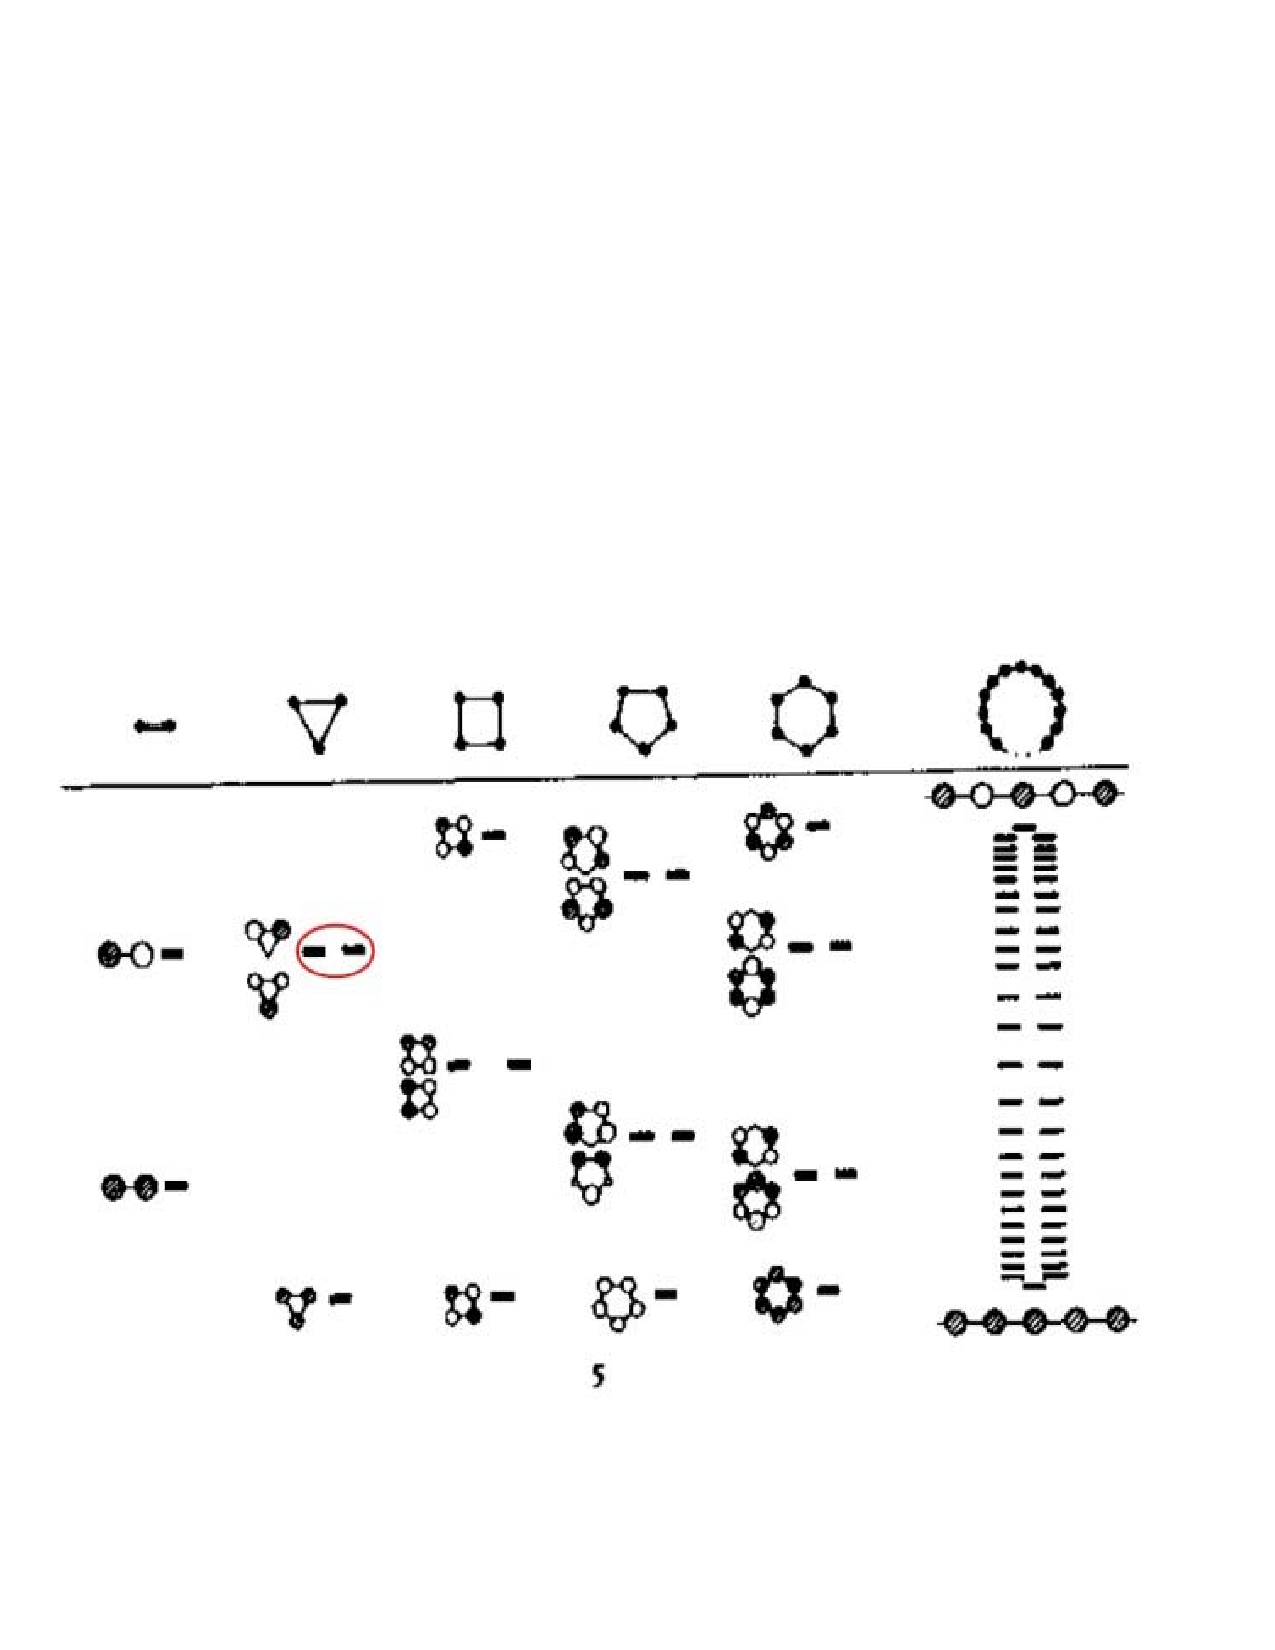
\includegraphics[height=0.8in,width=1.5in,viewport=30 140 545 480,clip]{Figures/Hydrogen-Mol-Orbital.pdf}}
\subfigure[分子波函数]{
\label{fig:Hydrogen-Psi}
\vspace*{-0.2in}
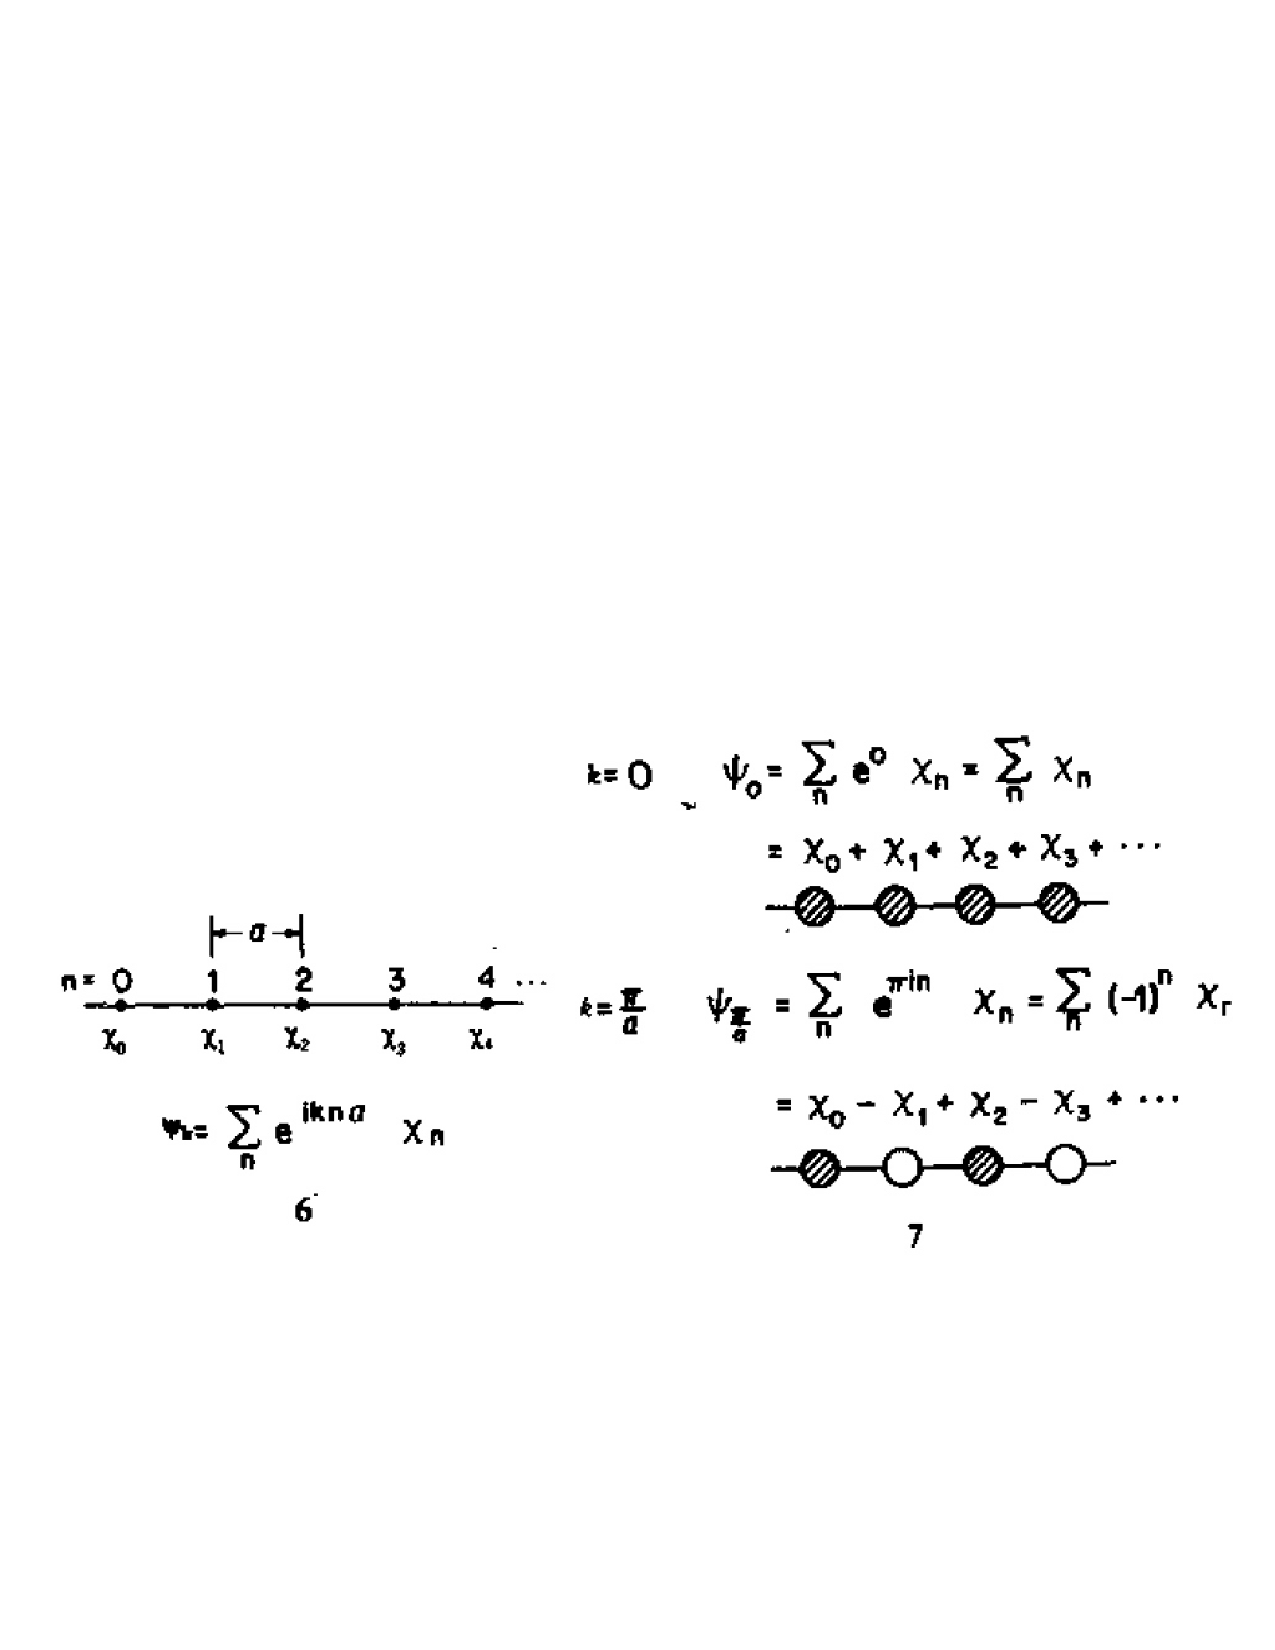
\includegraphics[height=0.5in,width=1.4in,viewport=25 218 595 440,clip]{Figures/Hydrogen-Psi.pdf}}\\
\subfigure[分子轨道与能带]{
\label{fig:Hydrogen-Band-1D}
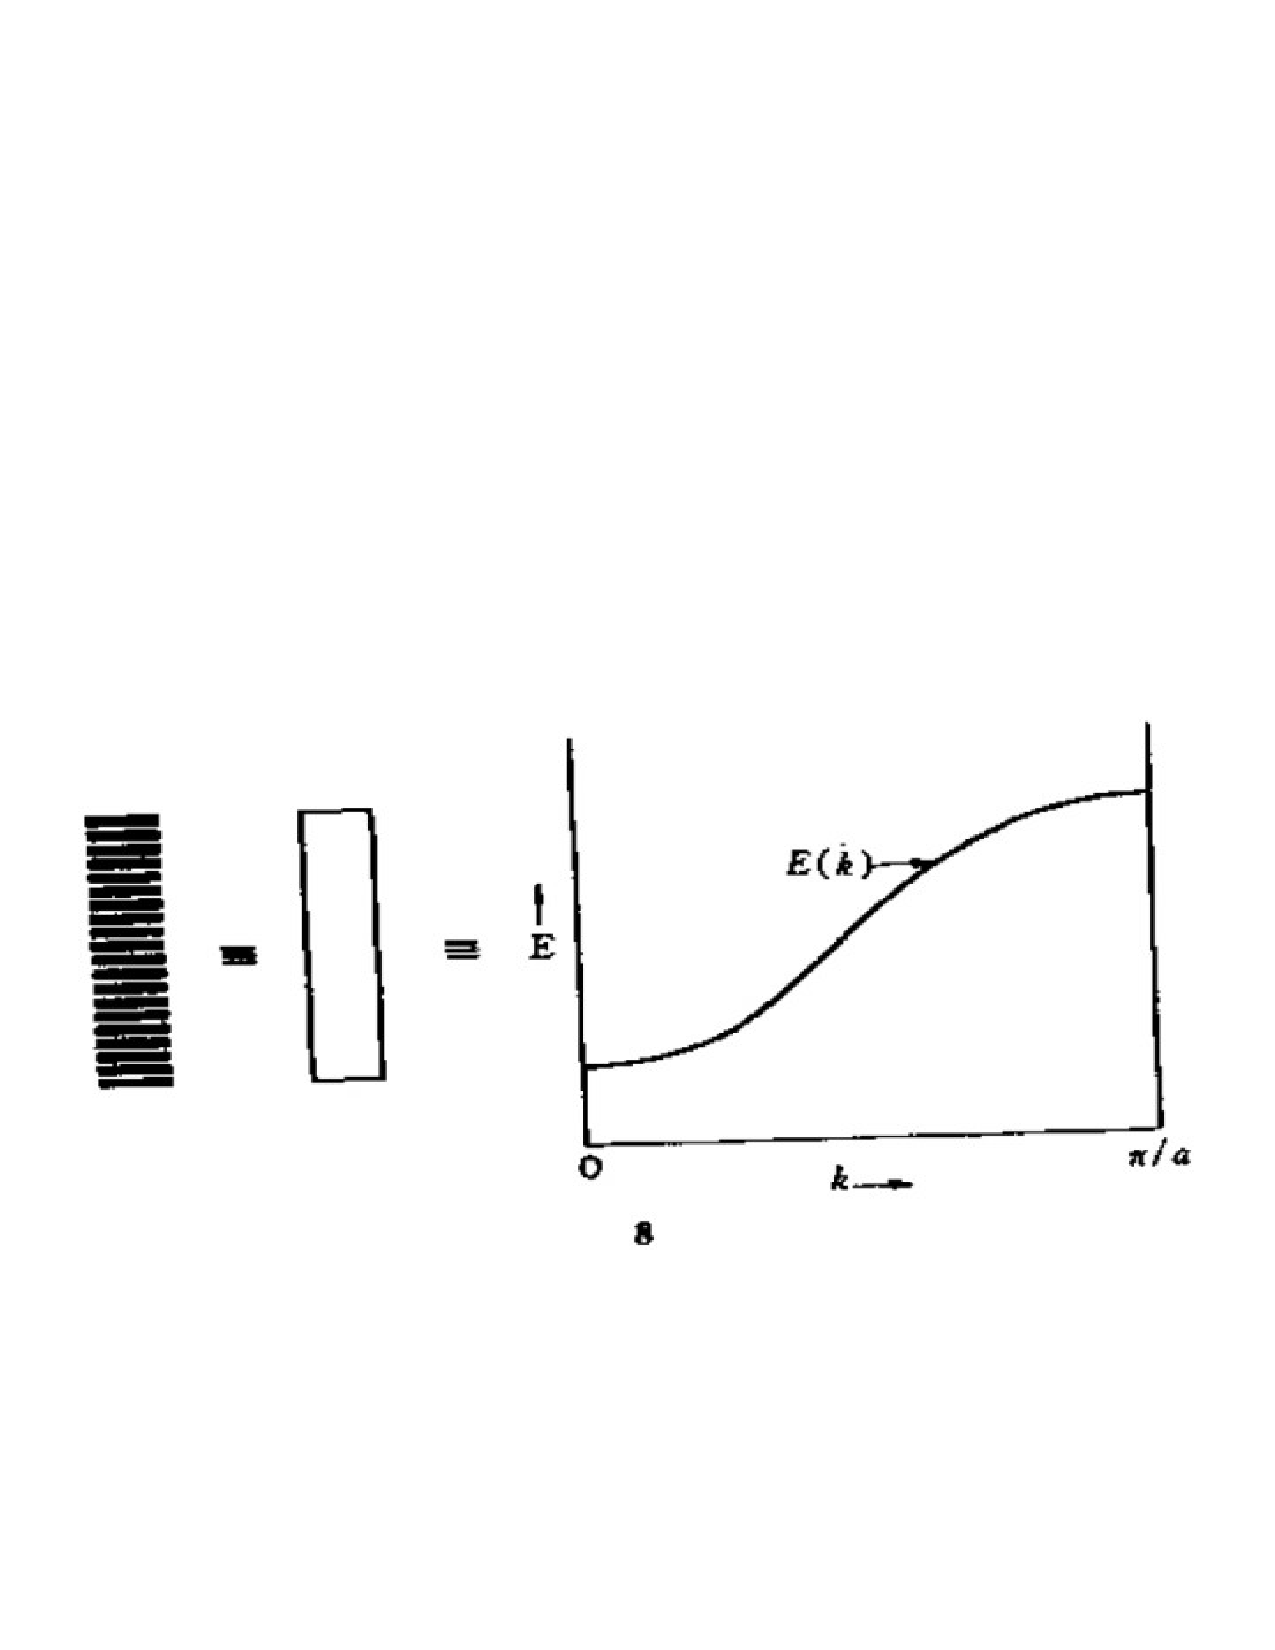
\includegraphics[height=0.6in,width=1.4in,viewport=35 215 575 450,clip]{Figures/Hydrogen-Band-1D.pdf}}
\subfigure[$d$\,轨道]{
\label{fig:Hydrogen-d-Band-1D}
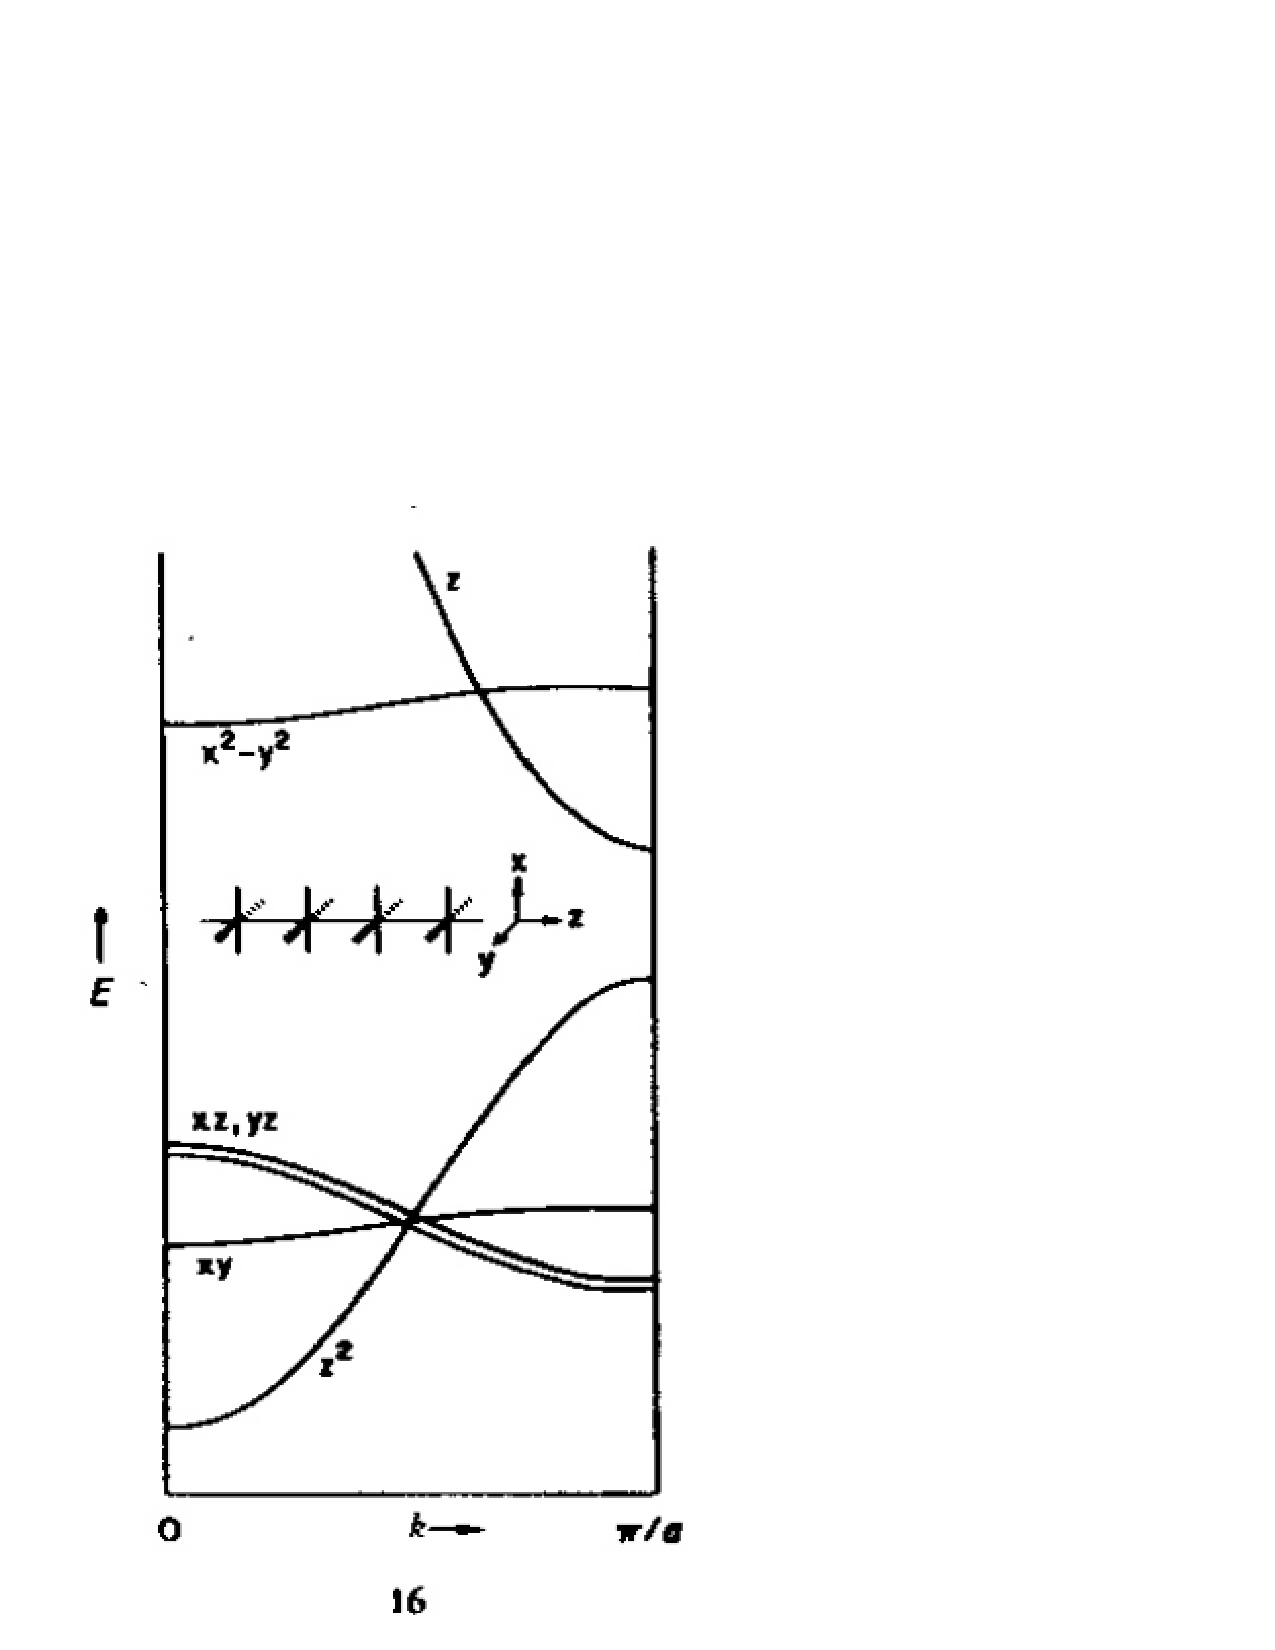
\includegraphics[height=1.0in,width=0.7in,viewport=40 45 330 535,clip]{Figures/Hydrogen-d-Band-1D.pdf}}
\caption{\small \textrm{The Band-structure from Molecular-orbital.}}%
\label{Band-Structure-1}
\end{figure} 
}

\frame
{
\frametitle{周期体系的波函数}
物质的电子体系,可分为芯层分子和价层电子。芯电子能量低,受周围化学环境影响很小,基本保持原子属性;价层电子相互作用较强,对化学环境较为敏感。一般地,价电子波函数在原子间区域(\textrm{Interstitial}区)的变化平缓,在临近原子核附近区域(\textrm{Muffin-tin}球内),会出现剧烈振荡(与芯层波函数正交)。
\begin{figure}[h!]
\centering
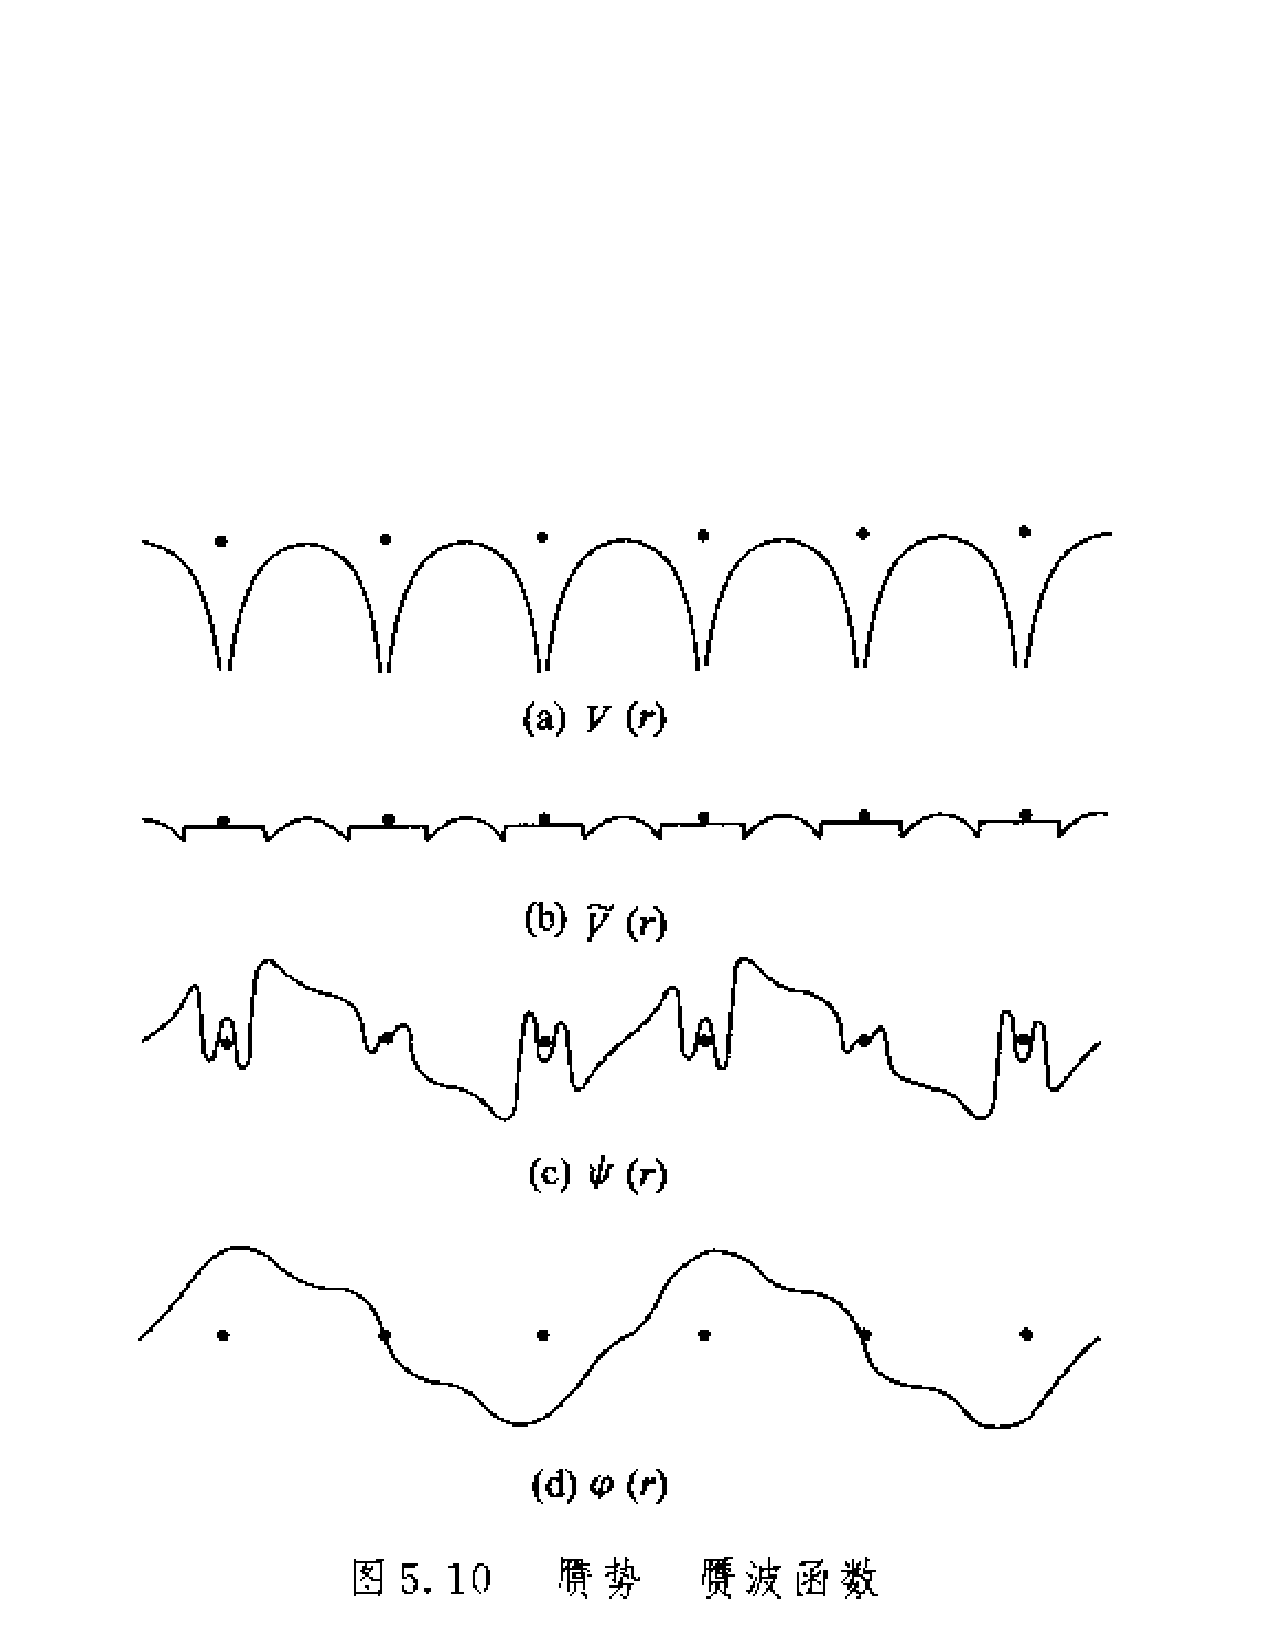
\includegraphics[height=0.8in,width=4.in,viewport=41 433 539 546,clip]{Figures/Pseudo_wave.pdf}\\
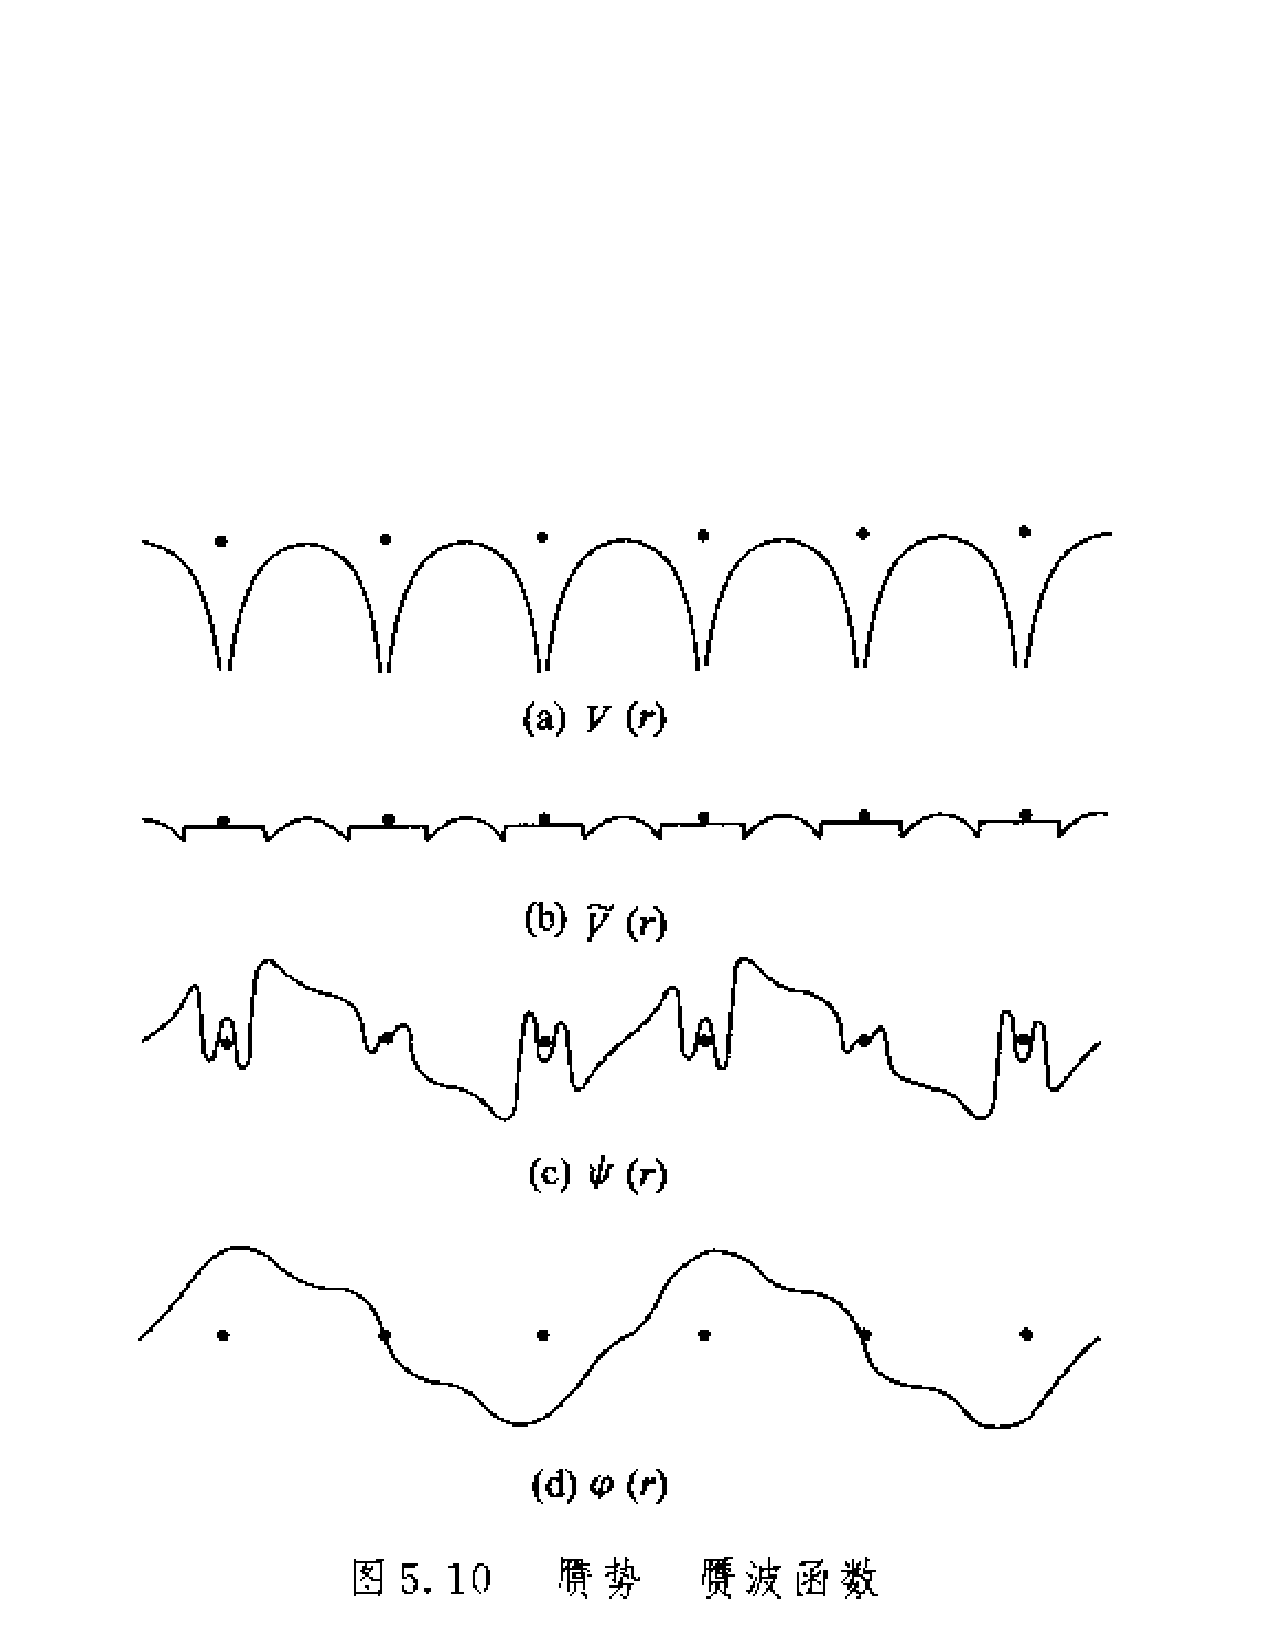
\includegraphics[height=0.8in,width=4.in,viewport=41 210 539 339,clip]{Figures/Pseudo_wave.pdf}
\caption{\small \textrm{The periodic Potential and the wave functions in crystal.}}%(与文献\cite{EPJB33-47_2003}图1对比)
\label{Potential-Wave}
\end{figure}
}

\frame
{
%\frametitle{The methods on band structure calculation}
\frametitle{固体能带计算方法}
%\vskip 10pt
%\textrm{The mainly difference of all these methods below: the basis sets and the construction of the potential}
\vskip 10pt
常用的计算方法
\begin{itemize}%[+-| alert@+>]
%\begin{enumerate}%[+-| alert@+>]
\setlength{\itemsep}{15pt}
%  \item \textrm{Plane wave and the pseudo-potential}
	\item	平面波方法
	\item	正交平面波\textrm{(The orthogonalized plane wave, OPW)}和赝势\textrm{(Pseudo-potential, PP)}方法\upcite{Singh_Book,PRB41-7892_1990,JPCM6-8245_1994}
	\item	缀加平面波\textrm{(Augmented plane wave, APW)}方法
	\item	\textrm{MT}轨道\textrm{(Muffin-tin orbitals, MTO)}方法
	\item	投影子缀加波\textrm{(Projector Augmented Wave, PAW)}方法\upcite{PRB50-17953_1994,PRB59-1758_1999}
\end{itemize}
  \vskip 5pt 各种方法的主要区别:所选的基函数类型不同
}

%\frame
%{
%\frametitle{}
%\begin{figure}[h!]
%\centering
%\vspace*{-10pt}
%\includegraphics[height=2.80in,width=1.70in,viewport=60 90 325 500,clip]{WIEN2k_Program_flow.eps}
%\caption{\small \textrm{Program flow in \textbf{WIEN2k}.}}%(与文献\cite{EPJB33-47_2003}图1对比)
%\label{WIEN2k_program_flow}
%\end{figure}
%}

\frame
{
%\frametitle{The methods on band structure calculation}
\frametitle{由OPW到赝势}
%\vskip 10pt
%\textrm{The mainly difference of all these methods below: the basis sets and the construction of the potential}
\begin{itemize}
\setlength{\itemsep}{5pt}
	\item 完全平面波基组,只要少数的平面波基组就可以很好地描述波函数在原子间的行为,近核的电子波函数则需要大量平面\\波展开。%因此完全平面波基组虽然方便,但求体系本征态对角化的矩阵非常巨大,计算变得异常耗时。
	\item 正交平面波(\textrm{Orthogonalized plane wave, OPW})方法,价电子用与芯层波函数正交的平面波展开,可以减少平面波数目
		\begin{displaymath}
			\phi_{OPW}^{\vec k+\vec G}(\vec r)=\phi_{PW}^{\vec k+\vec G}(\vec r)-\sum_{\alpha,c}\langle\varphi_c|\phi_{PW}^{\vec k+\vec G}\rangle\varphi_c(\vec r)
		\end{displaymath}
		并且势可以表示为$V^{eff}(\vec r)=V(\vec r)+V^R(\vec r)$,其中排斥部分是$$V^R(\vec r)=\sum_{\alpha,c}(\varepsilon_v-\varepsilon_c)|\varphi_c\rangle\langle\varphi_c|$$
\end{itemize}
}

\frame
{
\frametitle{赝势方法}
赝势(\textrm{Pseudo Potential, PP})方法是在正交平面波的基础上发展起来的,构造出平缓的势函数代替核的强吸引作用和芯层电子的排斥作用,用平缓的函数取代波函数近核时的震荡。
\begin{itemize}
\setlength{\itemsep}{5pt}
	\item 赝势-平面波方法,只需要少量平面波可展开赝波函数,大大提升了计算效率;但是赝波函数不能很好地反映与电子近核行为有关的性质。
	\item 赝势的构造并不唯一,考核构造赝势的两大指标:“柔软程度”\textrm{(Soft)}与“可移植性”\textrm{(transferability)}
\end{itemize}
\begin{figure}[h!]
\centering
\vspace*{-0.10in}
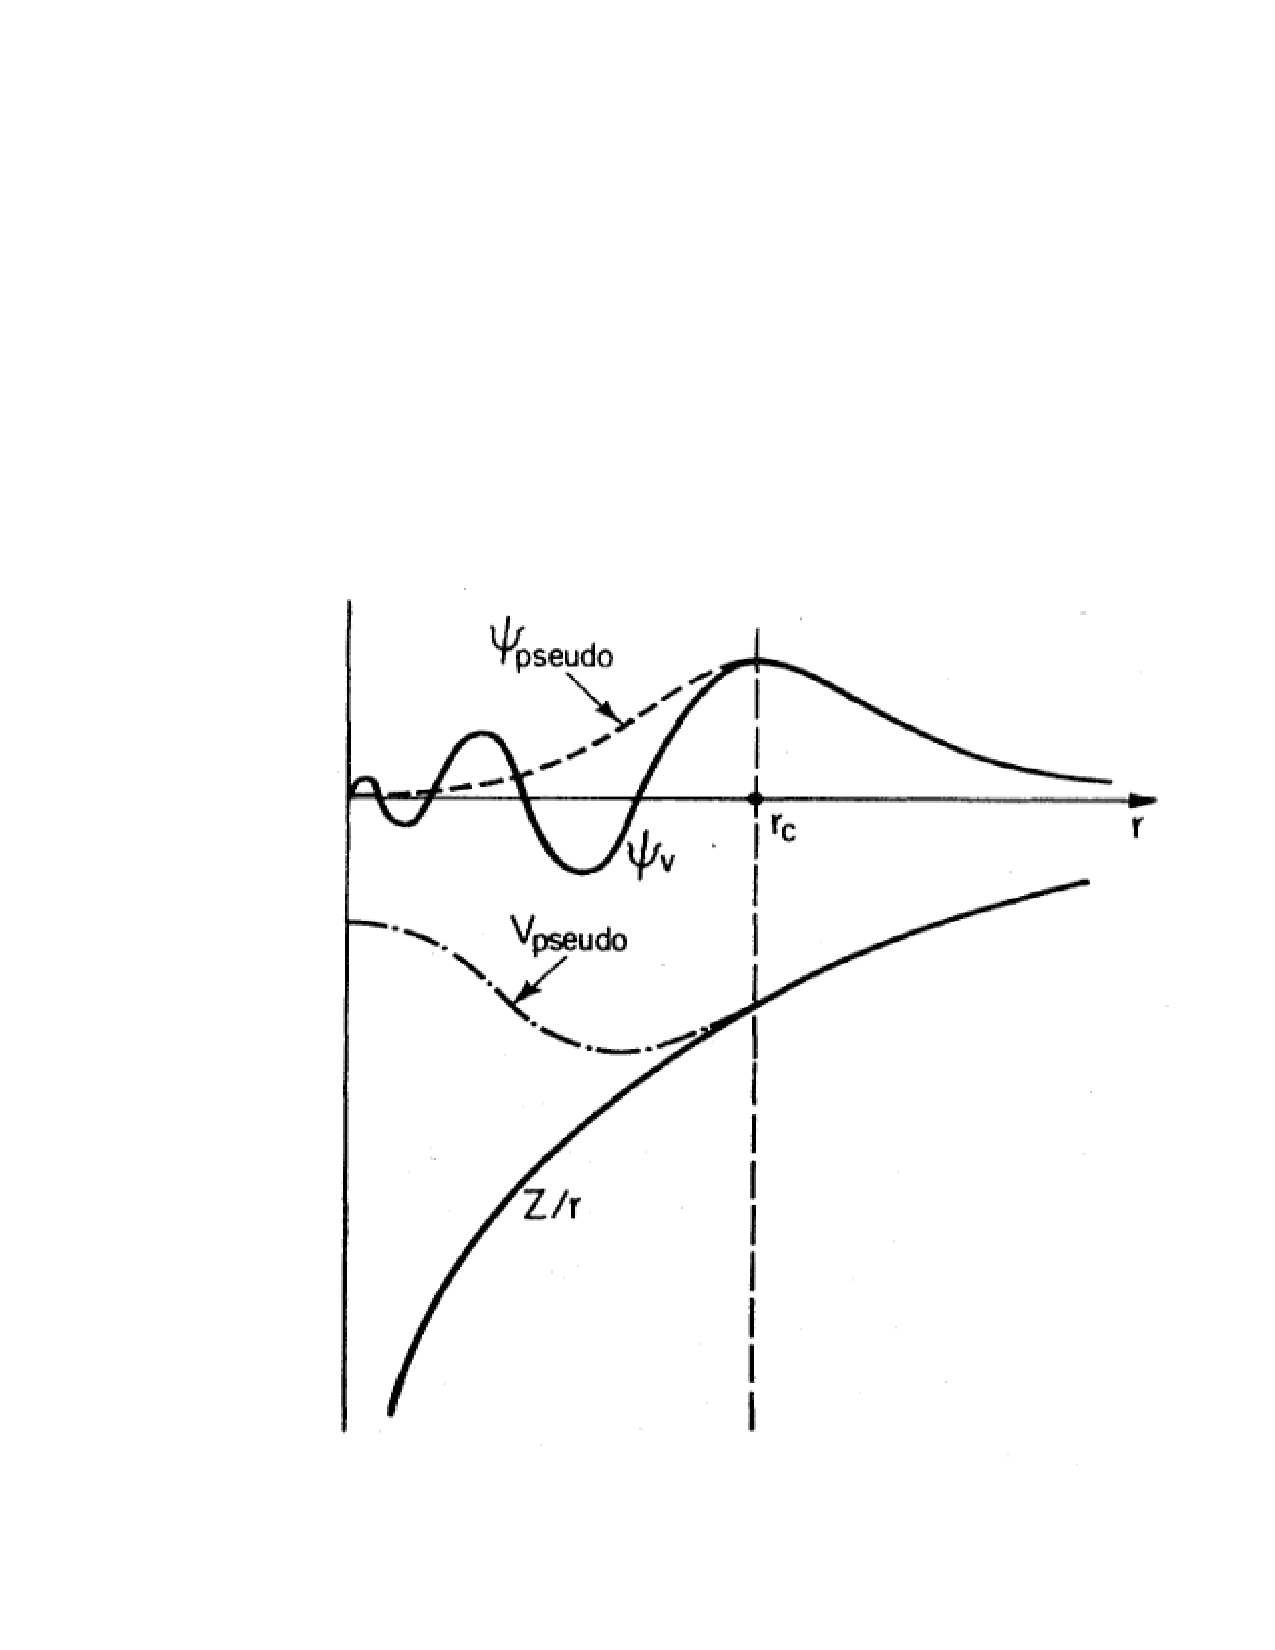
\includegraphics[height=1.35in,width=1.42in,viewport=154 100 562 508,clip]{Figures/Pseudo.pdf}
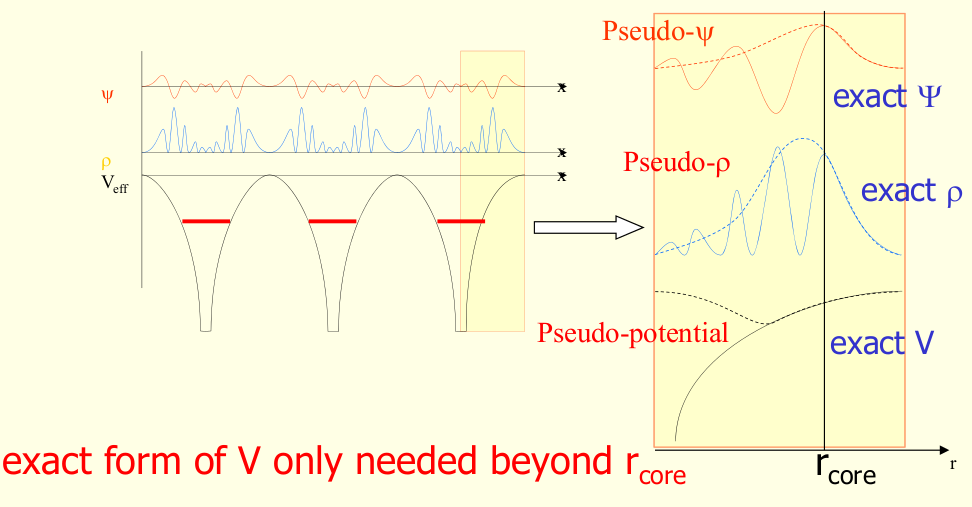
\includegraphics[height=1.35in,width=2.57in,viewport=1 1 980 500,clip]{Figures/Pseudo-2.png}
\caption{\small \textrm{The Pseudo wave function and Pseudo potential.}}%(与文献\cite{EPJB33-47_2003}图1对比)
\label{Pseudo_Potential-Wave}
\end{figure}
}

\frame
{
\frametitle{模守恒赝势和超软赝势}
\begin{itemize}
\setlength{\itemsep}{5pt}
	\item 模守恒\textrm{(Norm-conserving)}赝势,构造赝波函数有约束条件
		\begin{displaymath}
			\int_0^{r_c}\mathrm{d}\vec r\varphi^{\ast PS}(\vec r)\varphi^{PS}(\vec r)=\int_0^{r_c}\mathrm{d}\vec r\varphi^{\ast}(\vec r)\varphi(\vec r)
		\end{displaymath}
	模守恒赝势很好地解决了赝势的可移植性问题
	\item 超软\textrm{(Ultra-soft)}赝势,解除模守恒条件,实现对第一、第二周期元素的高效计算
\end{itemize}
\begin{figure}[h!]
\centering
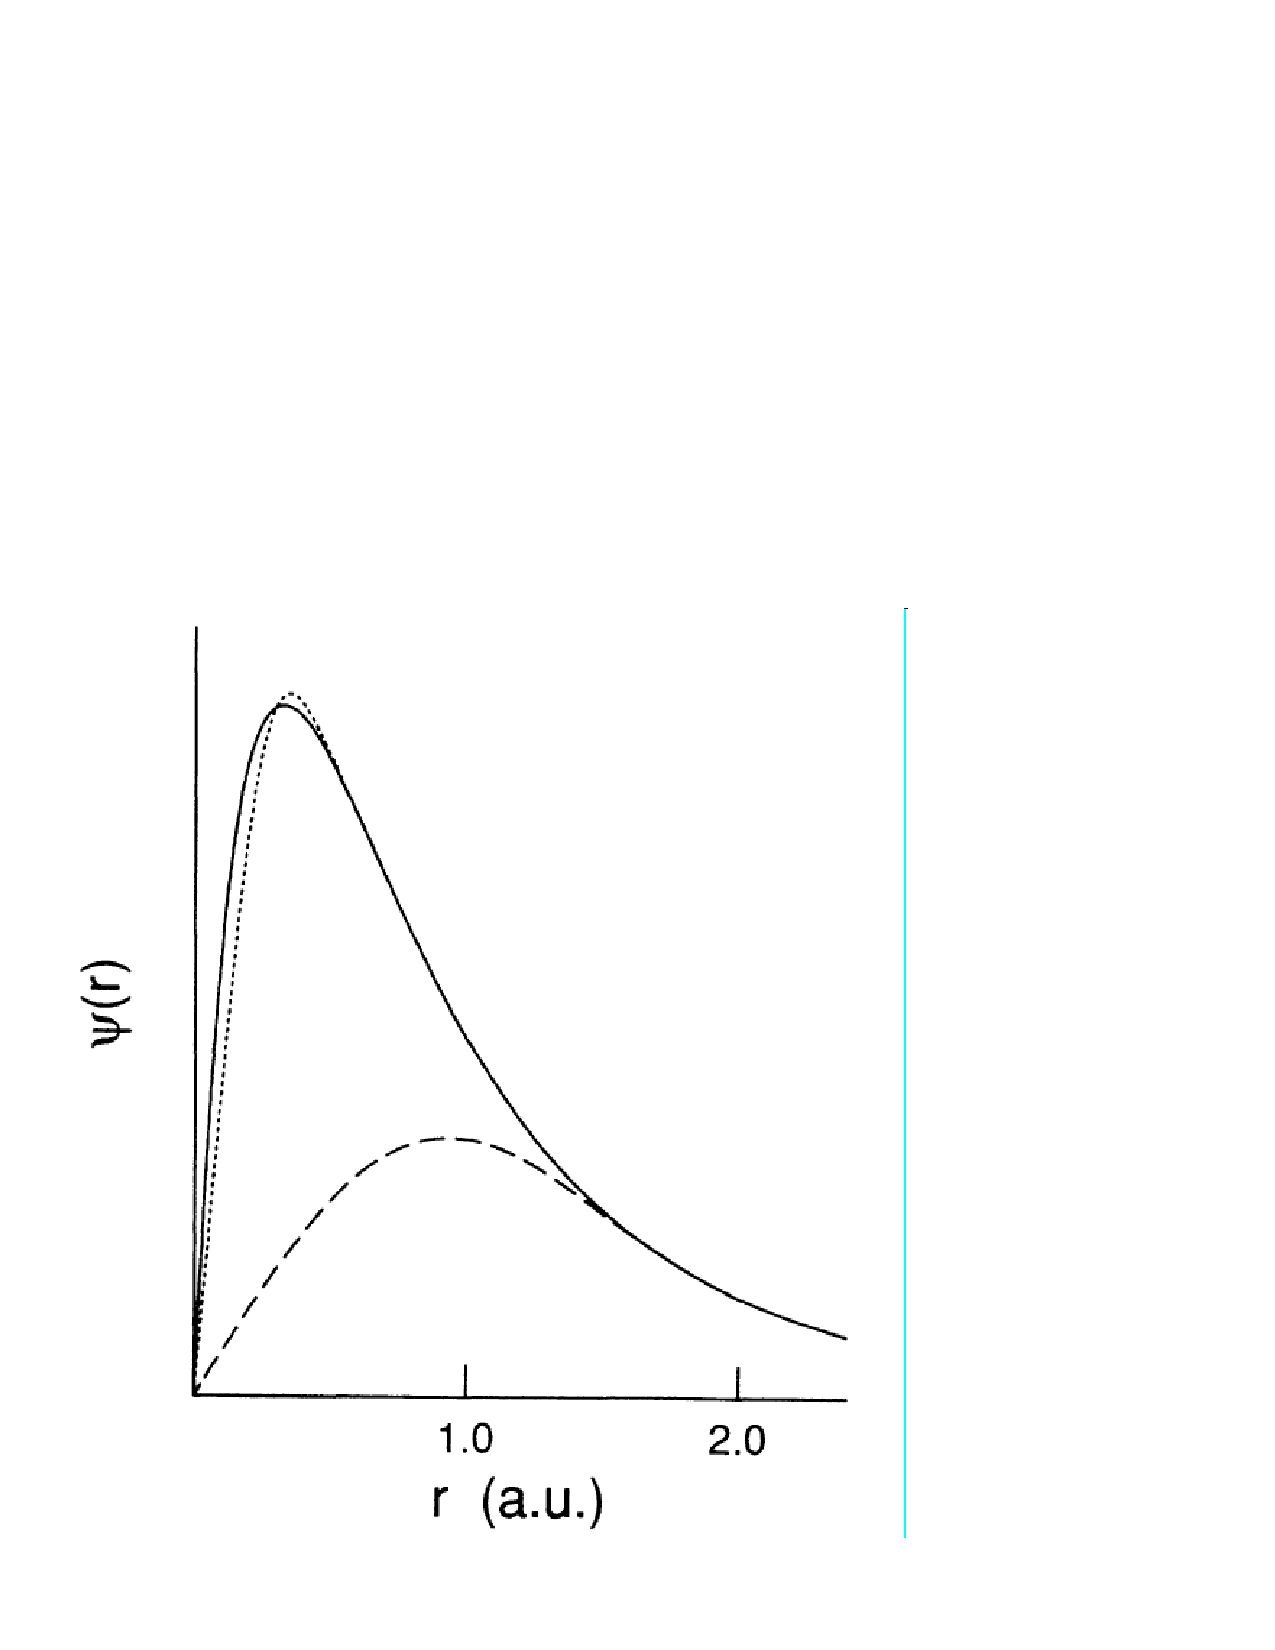
\includegraphics[height=1.35in,width=1.40in,viewport=30 55 415 500,clip]{Figures/Norm-US-wave.pdf}
\caption{\small \textrm{Oxygen 2} \textit{p} \textrm{radical wave function (solid), NC-pseudo-wave (dottde) and US-pseudo-wave (dashed).}}%(与文献\cite{EPJB33-47_2003}图1对比)
\label{Norm-US-wave}
\end{figure}
}

\frame
{
\frametitle{超软赝势}
超软赝势在平缓的局域势函数$V^L(\vec r)$和赝波函数$|\phi_{lmj}(\vec r)\rangle$的基础上,构造函数
\begin{displaymath}
	|\chi_{lmj}(\vec r)\rangle=\bigg[\varepsilon_{lj}-\dfrac12\nabla^2-V^L(\vec r)\bigg]|\phi_{lmj}(\vec r)\rangle
\end{displaymath}
在此基础上得到矩阵$\mathbf{B}_{ij}=\langle\phi_i|\chi_j\rangle$和局域函数
\begin{displaymath}
	|\beta_i\rangle=\sum_j(\mathbf{B}^{-1})_{ji}|\chi_{j}\rangle
\end{displaymath}
因此非局域赝势可以表示为
\begin{displaymath}
	V_{NL}=\dfrac{|\chi_i\rangle\langle\chi_i|}{\langle\chi_i|\chi_i\rangle}=\sum_{i,j}\mathbf{B}_{ij}|\beta_i\rangle\langle\beta_j|
\end{displaymath}
用平缓函数构造赝波函数与真实波函数的电荷密度差
\begin{displaymath}
	Q_{nm}(\vec r)=\varphi_n^{\ast}(\vec r)\varphi_m(\vec r)-\tilde\varphi_n^{\ast}(\vec r)\tilde\varphi_m(\vec r)
\end{displaymath}
}

\section{FP-LAPW方法}
\frame
{
\frametitle{\textrm{APW}方法和\textrm{LAPW}方法}
\begin{figure}[h!]
\centering
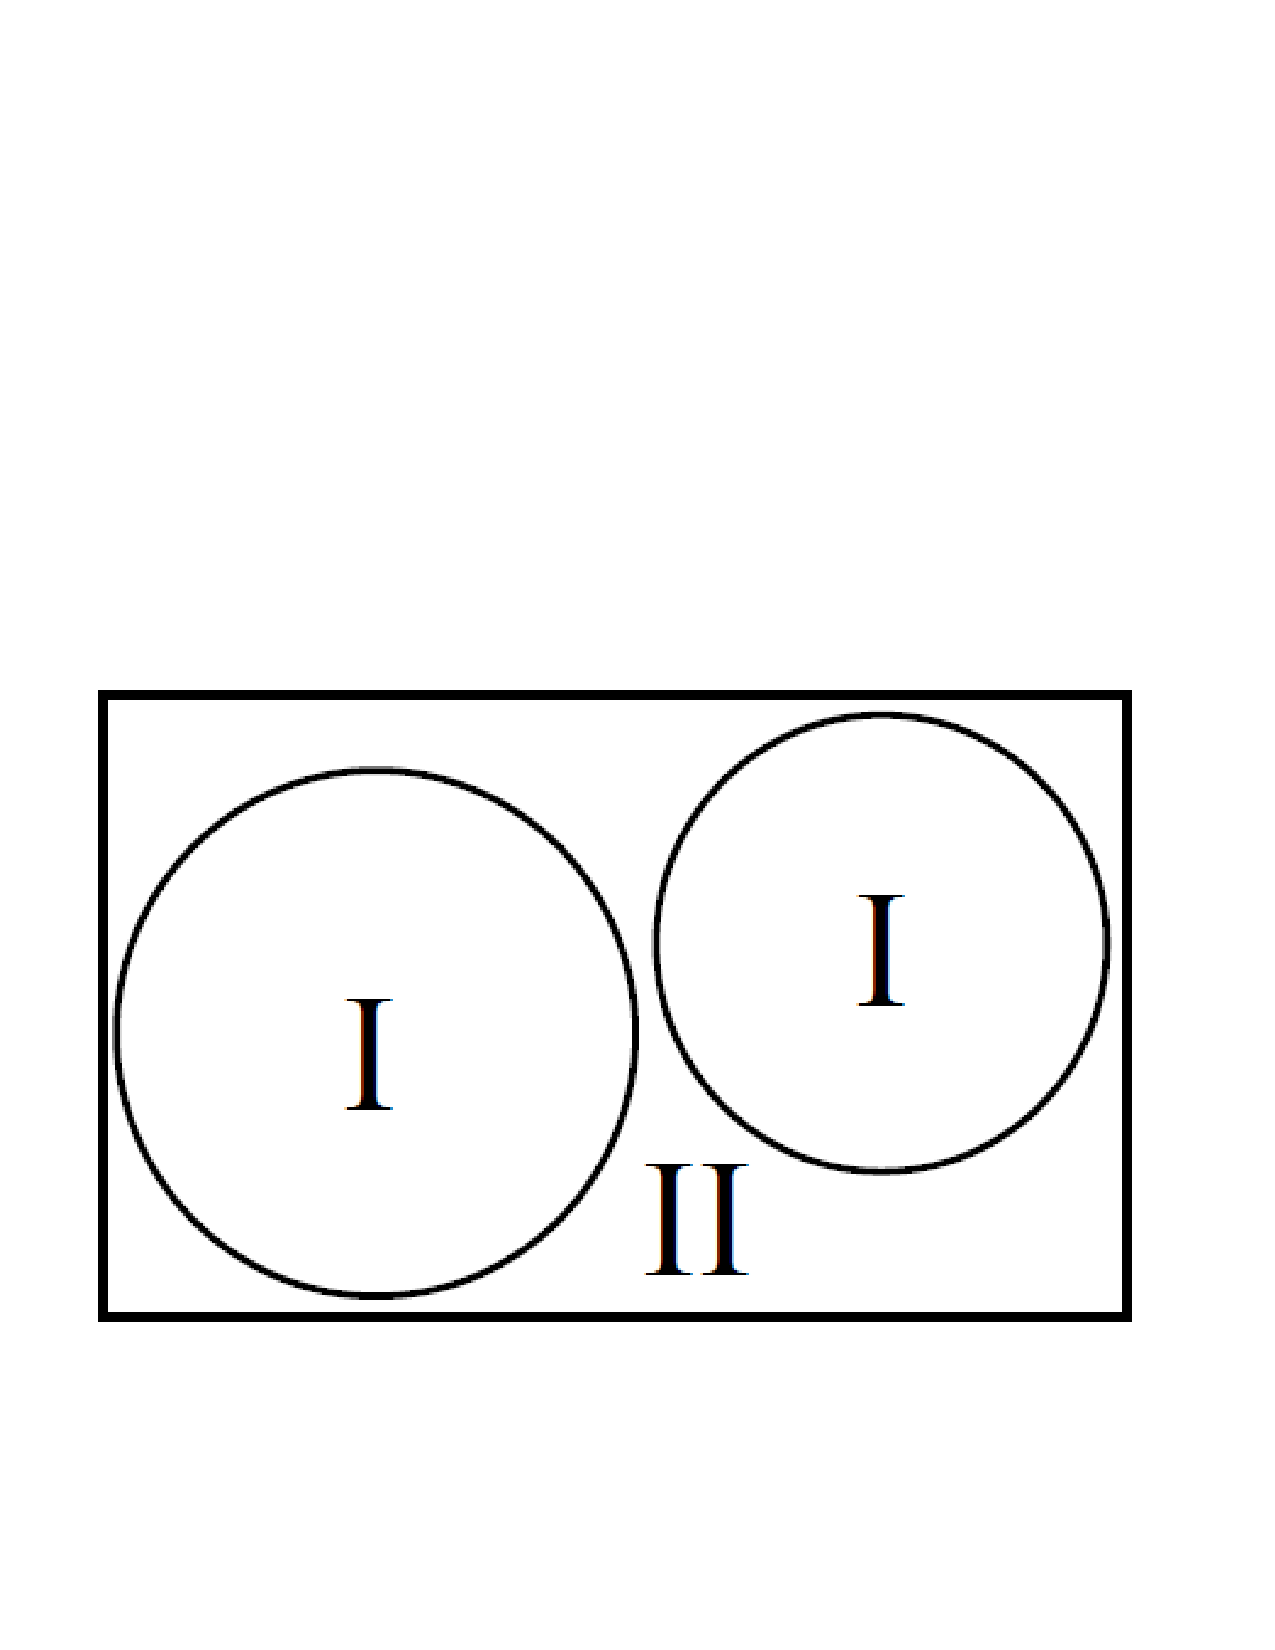
\includegraphics[height=1.10in,width=1.80in,viewport=40 150 545 465,clip]{Figures/Muffin_tin.pdf}
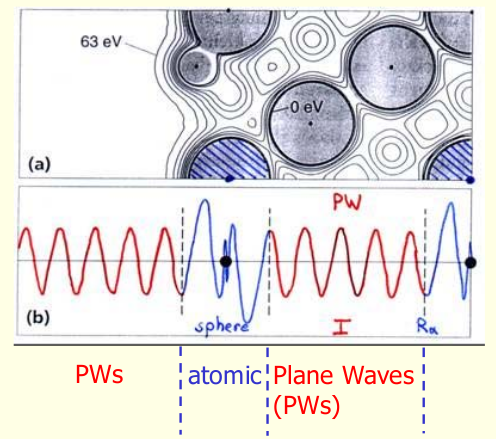
\includegraphics[height=1.10in,width=1.45in,viewport=1 20 485 435,clip]{Figures/APW.png}
\caption{\small \textrm{Partitioning of the unit cell into atomic spheres(I) and an interstitial region(II)}}%(与文献\cite{EPJB33-47_2003}图1对比)
\label{Muffin_tin}
\end{figure}
\begin{displaymath}
\hskip -28pt\footnotesize \varphi(\vec k_j,\vec r)=\left\{
  \begin{aligned}
    &\Omega^{-1/2}\exp[i\vec k_j\cdot\vec r],&|\vec r-\vec r_s|>R_{\mathrm{MT}}^s\\
    &\sum_{lm}A_{lm}u_l(|\vec r-\vec r_s|,E)Y_{lm}(\widehat{\vec r-\vec r_s}),&|\vec r-\vec r_s|\leqslant R_{\mathrm{MT}}^s
  \end{aligned}
\right.
\end{displaymath}
}

\frame
{
\frametitle{\textrm{APW}方法和\textrm{LAPW}方法}
%\small\textrm{APW}方法的困难,久期方程不能化成广义本征值方程的形式(久期方程对能量$E$是非线性的)为了克服这一困难,人们提出线性化方法,
\textrm{O.~K.~Andersen~}提出\textrm{LAPW}方法\upcite{Singh_Book}:将$u_l(r,E)$在某一合适的$E_l$值附近对$E$的一阶微商{\footnotesize$\left(\dfrac{\textrm{d}u_l(r,E)}{\textrm{d}E}\right)_{E_l}\equiv\dot u_l(r,E_l)$}\\代入\textrm{APW}基函数中可得\textrm{LAPW}方法的基函数:
$${\footnotesize\hskip -50pt \varphi(\vec k_j,\vec r)=\left\{
  \begin{aligned}
    &\Omega^{-1/2}\exp[i\vec k_j\cdot\vec r],&|\vec r-\vec r_s|>R_{\mathrm{MT}}^s\\
    &\sum_{lm}[A^{\vec k_j}_{lm}u_l(|\vec r-\vec r_s|,E_l)+B^{\vec k_j}_{lm}\dot u_l(|\vec r-\vec r_s|,E_l)]Y_{lm}(\widehat{\vec r-\vec r_s}),&|\vec r-\vec r_s|\leqslant R_{\mathrm{MT}}^s
  \end{aligned}
\right.}$$
%$$\Psi_{\vec k}(\vec r)=\int_{\Omega}\tilde G_{\vec k}(\vec r-\vec r\,^\prime;E)V(\vec r\,^\prime)\Psi_{\vec k}(\vec r\,^\prime)\textrm{d}\vec r\,^\prime$$
根据基函数在\textrm{MT}球面上连续到一阶,确定系数$A^{\vec k}_{lm}$,$B^{\vec k}_{lm}$的值。
\begin{figure}[h!]
\centering
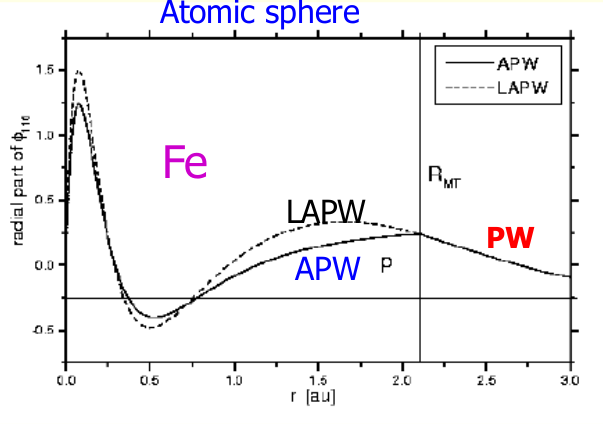
\includegraphics[height=1.20in,width=1.98in,viewport=1 20 585 435,clip]{Figures/WIEN2k-LAPW.png}
\caption{\small \textrm{Partitioning of the unit cell into atomic spheres(I) and an interstitial region(II)}}%(与文献\cite{EPJB33-47_2003}图1对比)
\label{Muffin_tin}
\end{figure}
}
\frame
{
\frametitle{\textrm{LO}基函数}
为提高\textrm{LAPW}方法的变分自由度,在同一能量范围处理半芯态(接近价态的能量较高的芯态)和价态,可添加与$\vec k$无关的基函数,称为局域轨道(\textrm{local orbitals, LO})%。据此构造的基函数称为%包含两个指定能量的径向波函数和其中一个能量导数,这样的基函数即LAPW+
或\textrm{LO}基函数:
{\footnotesize
$$\hskip -40pt \phi_{lm}^{\mathrm{LO}}(\vec r)=\left\{
  \begin{aligned}
    &[A_{lm}u_l(r,E_{1,l})+B_{lm}\dot u_l(r,E_{1,l})+C_{lm}u_l(r,E_{2,l})]Y_{lm}(\hat{\vec r})\quad&r\leqslant R_{\mathrm{MT}}^s\\
    &0 &r>R_{\mathrm{MT}}^s
\end{aligned}
\right.$$}

类似地,根据$\phi_{lm}^{\mathrm{LO}}(\vec r)$在\textrm{MT}球面上的数值为零、一阶导数为零,并且$\phi_{lm}^{\mathrm{LO}}(\vec r)$在\textrm{MT}球内归一化的要求,可以确定系数$A_{lm}$,$B_{lm}$,$C_{lm}$的值。
\begin{figure}[h!]
	\vspace{-15pt}
\centering
\hspace{15pt}
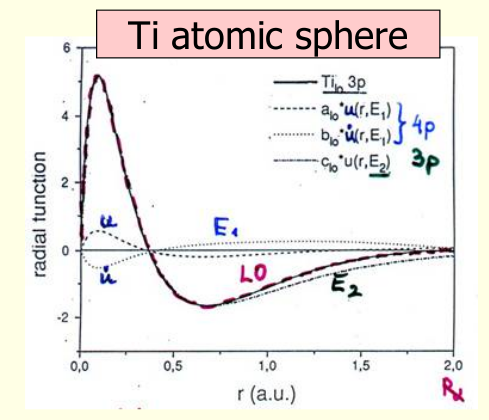
\includegraphics[height=1.45in,width=1.55in,viewport=50 10 470 415,clip]{Figures/WIEN2k-lo.png}
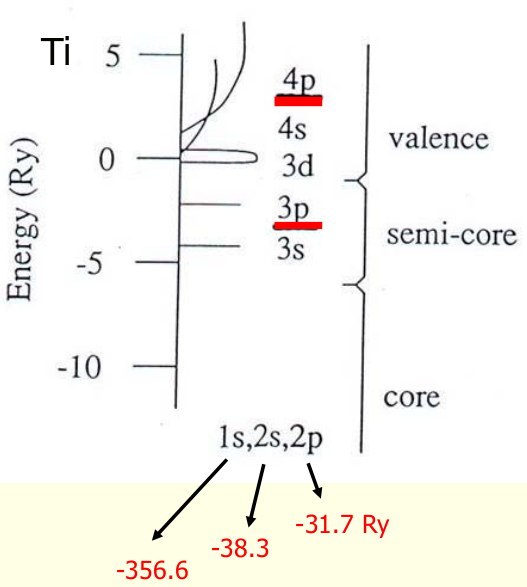
\includegraphics[height=1.45in,width=1.45in,viewport=5 1 570 570,clip]{Figures/semi-core.png}
\caption{\small \textrm{}}%(与文献\cite{EPJB33-47_2003}图1对比)
\label{Muffin_tin_LO}
\end{figure}
}

\frame
{
\frametitle{\textrm{APW+lo}基函数}
\textrm{Sj\"ostedt}等发现上述\textrm{LAPW}方法并非是\textrm{APW}方法线性化的最有效方法。采用指定能量参数$E_l$的\textrm{APW}形式的径向波函数,外加\textrm{APW}型局域轨道(\textrm{local orbit, lo})基函数,是更有效的方案,称为\textrm{APW+lo}方法\upcite{SSC114-15_2000}。
$$  \varphi(\vec k_j,\vec r)=\left\{
  \begin{aligned}
    &\sum_{lm}[A^{\vec k_j}_{lm}u_l(r,E_l)]Y_{lm}(\hat{\vec r})\quad&r\leqslant R_{\mathrm{MT}}^s\\
    &\Omega^{-1/2}\exp(i\vec k_j\cdot\vec r) &r>R_{\mathrm{MT}}^s
  \end{aligned}\right.
  \label{eq:APW-basis}
$$
$$  \phi_{lm}^{\mathrm{lo}}(\vec r)=\left\{
  \begin{aligned}
  &[A_{lm}u_l(r,E_{1,l})+B_{lm}\dot u_l(r,E_{1,l})]Y_{lm}(\hat{\vec r})\quad&r\leqslant R_{\mathrm{MT}}^s\\
  &0&r>R_{\mathrm{MT}}^s
  \end{aligned}
\right.$$
\textrm{APW+lo}基函数式形式上与标准\textrm{LAPW}基函数式形式非常相似,但\textrm{APW+lo}基函数是平滑且一阶可微的,在\textrm{MT}球面上有动能对\textrm{Hamiltonian}的贡献需要计算。计算表明,采用\textrm{APW+lo}基组比标准\textrm{LAPW}基组计算效率高。
}

\frame
{
\frametitle{\textrm{WIEN2k}程序中基函数的选择}
\vskip 10pt
\begin{itemize}
\setlength{\itemsep}{15pt}
	\item 对$s$态、$p$态价电子轨道用\textrm{LAPW}基组展开
	\item 对一般平面波基函数展开收敛缓慢的轨道(如过渡金属的3$d$态波函数)或\textrm{MT}球半径特别小的体系用\textrm{APW+lo}基组展开
	\item 对半芯层轨道用\textrm{LAPW-LO}基组展开
\end{itemize}
这样搭配选择基组,可以同时较好地处理价态和半芯态。
}

\frame
{
\frametitle{\textrm{WIEN2k}程序中基函数的选择}
\begin{figure}[h!]
	\vspace{-15pt}
\centering
\hspace{15pt}
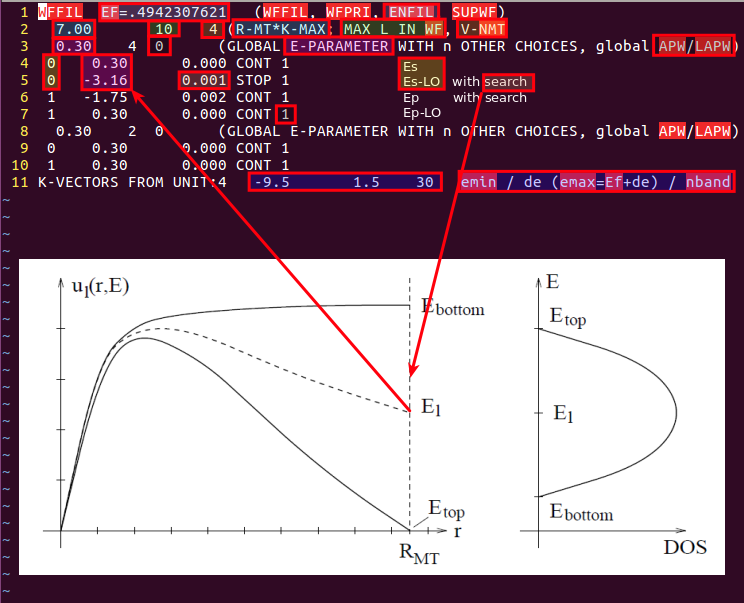
\includegraphics[height=2.55in,width=3.35in,viewport=10 30 750 605,clip]{Figures/WIEN2k-in1.png}
\caption{\small \textrm{The parameter $\mathrm{E}_l$ in case.in1 for WIEN2k.}}%(与文献\cite{EPJB33-47_2003}图1对比)
\label{WIEN2k-in1}
\end{figure}
}

\frame
{
\frametitle{全势的基本思想}
全势\textrm{(Full Potential, FP)}是相对于赝势的概念,即\textcolor{blue}{电子运动过程中感受到其它粒子作用的真实效果}。
实际计算中,构造\textrm{LAPW}基组的\textrm{MT}势换成晶体势函数。一般地,在每个\textrm{MT}球内,势函数用球谐函数(或者是满足晶体对称性)展开,\textrm{MT}球外的势函数用\textrm{Fourier}级数展开:%\upcite{PRB13-5362_1976}
{\footnotesize$$ V(\vec r)=\left\{
  \begin{aligned}
    &\sum_{a,L}V_L^a(r)Y_L(\hat{\vec r})\quad &r\leqslant R_{\mathrm{MT}}^a\\
    &\sum_{\vec G_n}V_I(\vec G_n)\textrm{e}^{i\vec G_n\cdot\vec r} &\vec r\in\mathrm{II}
  \end{aligned}\right.
  \label{eq:solid-63}
$$}
这里$L$\,$\equiv$\,$l,m$,$\vec G_n$为倒格矢,$Y_L(\hat{\vec r})$是球谐函数,\textrm{II}为原子间区域。
\begin{itemize}
	\item 在\textrm{MT}球内靠近原子核,势能具有原子型势能特征
	\item 在\textrm{MT}球外,要满足\textrm{Bloch}函数边界条件特征。
	\item 在\textrm{MT}球内外的势能表象不同,同样要求势能在\textrm{MT}球表面连续。
\end{itemize}
}

\frame
{
\frametitle{全势的基本思想}
\vspace*{-13pt}
\begin{figure}[h!]
\centering
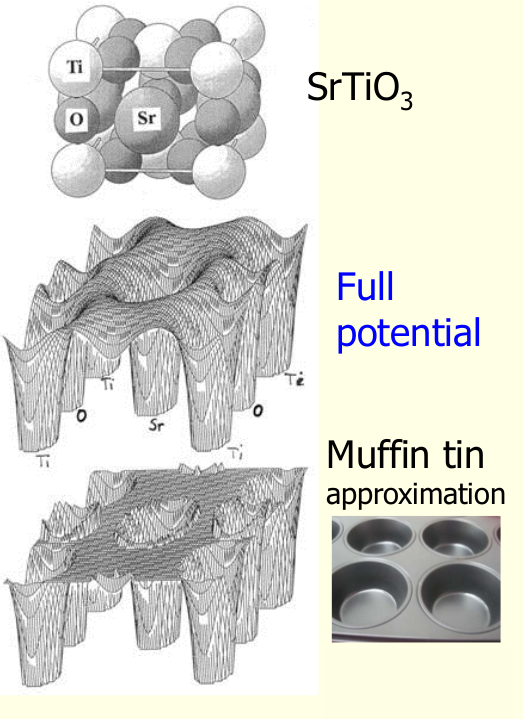
\includegraphics[height=2.70in,width=2.02in,viewport=1 22 507 715,clip]{Figures/MT_FP.png}
\caption{\small \textrm{From Muffin-tin Potential to Full Potential}}%(与文献\cite{EPJB33-47_2003}图1对比)
\label{Muffin_tin_LO}
\end{figure}
}

\frame
{
\frametitle{全势的基本思想}
由此得到晶体的势函数为\upcite{Comp_Method}
$$ V(\vec r)=V_{MT}(\vec r)+V_{WMT}(\vec r)+V_{NS}(\vec r)
  \label{eq:solid-64}
$$
\begin{itemize}
	\item $V_{MT}(\vec r)$是简单的\textrm{MT}势(包括\textrm{MT}球内球对称部分和\textrm{MT}球外常数势)
	\item $V_{WMT}(\vec r)$表示\textrm{MT}球外势能\textrm{Fourier}展开对\textrm{MT}常数势的偏离,仅在\textrm{MT}球外非零,球内为零
	\item $V_{NS}(\vec r)$是势能在\textrm{MT}球内对球对称性的偏离,只在\textrm{MT}球内有非零值
\end{itemize}
\textbf{\large 为求得交换-相关势$V_{XC}$,将电荷密度也采用类似的形式展开。}
}
\frame
{
\frametitle{全势方法在$\vec k$空间中的实现}
\textrm{WIEN2k}程序包采用\textrm{Weiner}提出全势计算方法\upcite{JMP22-2433_1981}。
\begin{itemize}
	\item 将\textrm{MT}球外的电荷密度(常数)扩展到球内,并在正空间内作多极矩展开$Q_{PW}(\vec r)\quad(r\leqslant R_{\mathrm{MT}}^s)$
	\item 根据\textrm{MT}球内的电荷密度分布,电子密度在正空间分布的多极矩$Q_{MT}(\vec r)\quad(r\leqslant R_{\mathrm{MT}}^s)$
	\item 构造赝电荷密度$\tilde\rho(\vec r)$,要求$\tilde\rho(\vec r)$在空间分布平缓(方便\textrm{Flourier}变换),其多级矩$\tilde Q_{MT}(\vec r)\quad(r\leqslant R_{\mathrm{MT}}^s)$为真实电荷密度多极展开多极矩与延伸到球内的电荷多极矩之差\\
	\item 在$\vec k$空间内,体系\textrm{MT}球外真实电荷密度叠加\textrm{MT}球内赝电荷密度,根据\textrm{Coulomb}定理计算得到\textrm{Coulomb}势在间隙区的表达式$V_C(\vec k)$
	\item 以\textrm{MT}球面的势能为球形\textrm{Dirichlet}边值条件,计算\textrm{MT}球内电子的\textrm{Coulomb}势$V(\vec r)$
\end{itemize}
}
\frame
{
\frametitle{总能量的计算}
\textrm{WIEN2k}程序中,\textrm{WS}原胞内的总能量可以表示为\upcite{PRB26-4571_1982}:
{\footnotesize
\begin{displaymath}
\begin{split}
E_T=&\sum_i\varepsilon_i-\frac12\int_{\Omega}\rho(\vec r)[V_C(\vec r)+2\mu_{XC}(\vec r)]\mathrm{d}\vec r-\frac12\sum_{\nu}Z_{\nu}V_M(\vec r_{\nu})+E_{XC}[\rho] \\
   =&\sum_i\varepsilon_i-\frac12\left(\int_{\Omega}\rho(\vec r)V_C(\vec r)\mathrm{d}\vec r+\sum_{\nu}Z_{\nu}\bigg\langle\frac1r\rho(\vec r)\bigg\rangle_{\nu}\right)-%\dfrac12
   \int_{\Omega}\rho(\vec r)\mu_{XC}(\vec r)\mathrm{d}\vec r \\
   &-\frac12\sum_{\nu}\frac{Z_{\nu}}{R_{\nu}}[R_{\nu}S_0(R_{\nu})+Z_{\nu}-Q_{\nu}]+E_{XC}[\rho]
\end{split}
\end{displaymath}
}
这里$V_C(\vec r)\!=\!\displaystyle\int\dfrac{\rho(\vec r\,^\prime)}{|\vec r-{\vec r}\,^\prime|}\mathrm{d}\vec r\,^\prime-\sum\limits_{\alpha}\dfrac{Z_{\alpha}}{|\vec r-\vec r_{\alpha}|}$,$\mu_{XC}$为交换-相关势。
}
\frame
{
\frametitle{原子核位置能量奇点排除}
核吸引势和\textrm{Coulomb}势在原子核位置都存在奇点,单独求和,总能量是发散的。

为排除奇点,将\textrm{Coulomb}势能和电荷密度在各原子核附近用球谐函数展开,在原子核附近,有
{\footnotesize\begin{displaymath}
  \begin{split}
    &\int_{\Omega}\rho(\vec r)V_C(\vec r)\mathrm{d}\vec r+Z_{\nu}\sqrt{4\pi}\int_0^{R_{\nu}}\mathrm{d}rr^2\frac{\rho_{00}(r)}r\\
    =&\sqrt{4\pi}\int_{\Omega}\mathrm{d}rr^2\rho_{00}(\vec r)\left(\dfrac1{\sqrt{4\pi}}V_{00}(r)+\frac{Z_{\nu}}r\right)+\sum_{lm>0}\int\mathrm{d}rr^2\rho_{lm}(r)V_{lm}(r)
  \end{split}
\end{displaymath}}
\textrm{Coulomb}势的奇点只出现在$V_{00}(r)$中,将$V_{00}(r)$写成核的点电荷势与源于电子的平缓的势$\hat V_{00}(r)$两部分之和,
\footnotesize{$$V_{00}(r)=-\sqrt{4\pi}\frac{Z_{\nu}}r+\hat V_{00}(r)$$}
可以看出\textrm{Coulomb}势的奇点被消去了。\\有必要指出的是,这样方式可以将总能量中的奇点排除,但是单独每一项在原子核位置仍然是发散的。
}
\frame
{
\frametitle{LDA近似下的总能量表达式}
\begin{itemize}
	\item 间隙区的电荷密度用平面波展开:\footnotesize{$\rho(\vec r)=\sum\limits_{\vec G}\rho(\vec G)\mathrm{e}^{i\vec G\cdot\vec r}$}
	\item 在\textrm{MT}球内,电荷密度用球谐函数展开,在动量空间中的展开形式为:\footnotesize{$\bar\rho_{lm}(r_{\nu})=4\pi i^l\sum\limits_{\vec G}\rho(\vec G)\mathrm{e}^{i\vec G\cdot\vec r_{\nu}}j_l(\vec G\cdot\vec r_{\nu})Y_{lm}^{\ast}(\vec G)$}
\end{itemize}
\textrm{LDA}近似下,\footnotesize{$$E_{XC}[\rho]\approx\int_{\Omega}\rho(\vec r)\varepsilon_{XC}(\vec r)\textrm{d}\vec r$$}
因此\textrm{WS}原胞内的晶体总能量可以写成:
{\footnotesize
\begin{displaymath}
  \begin{split}
\hskip -10pt	  E=&\sum_i\varepsilon_i-\Omega\sum_{\vec G}\rho(\vec G)\tilde V^{\ast}(\vec G)-\frac12\sum_{\nu}\dfrac{Z_{\nu}}{R_{\nu}}[Z_{\nu}-Q_{\nu}+R_{\nu}S_0(R_{\nu})]\\
    &-\sum_{\nu}\sum_{lm}\int_0^{R_{\nu}}\mathrm{d}rr^2\left[\rho_{lm}(r_{\nu})\left(\tilde V_{lm}^{\ast}(r_{\nu})+\dfrac{\sqrt{4\pi}}{2r_{\nu}}Z_{\nu}\delta_{l0}\right)-\bar\rho_{lm}(\vec r_{\nu})\bar V_{lm}^{\ast}(\vec r_{\nu})\right]
  \end{split}
  \label{eq:solid-83}
\end{displaymath}}
这里$\tilde V(\vec r)$和$\bar V_{lm}(\vec r)$根据都按下式计算:
\footnotesize{$$\tilde V(\vec r)=\frac12V_C(\vec r)-\varepsilon_{XC}(\vec r)+\mu_{XC}(\vec r)$$}
}

\frame
{
\frametitle{}
\begin{figure}[h!]
\centering
\hspace*{-10pt}
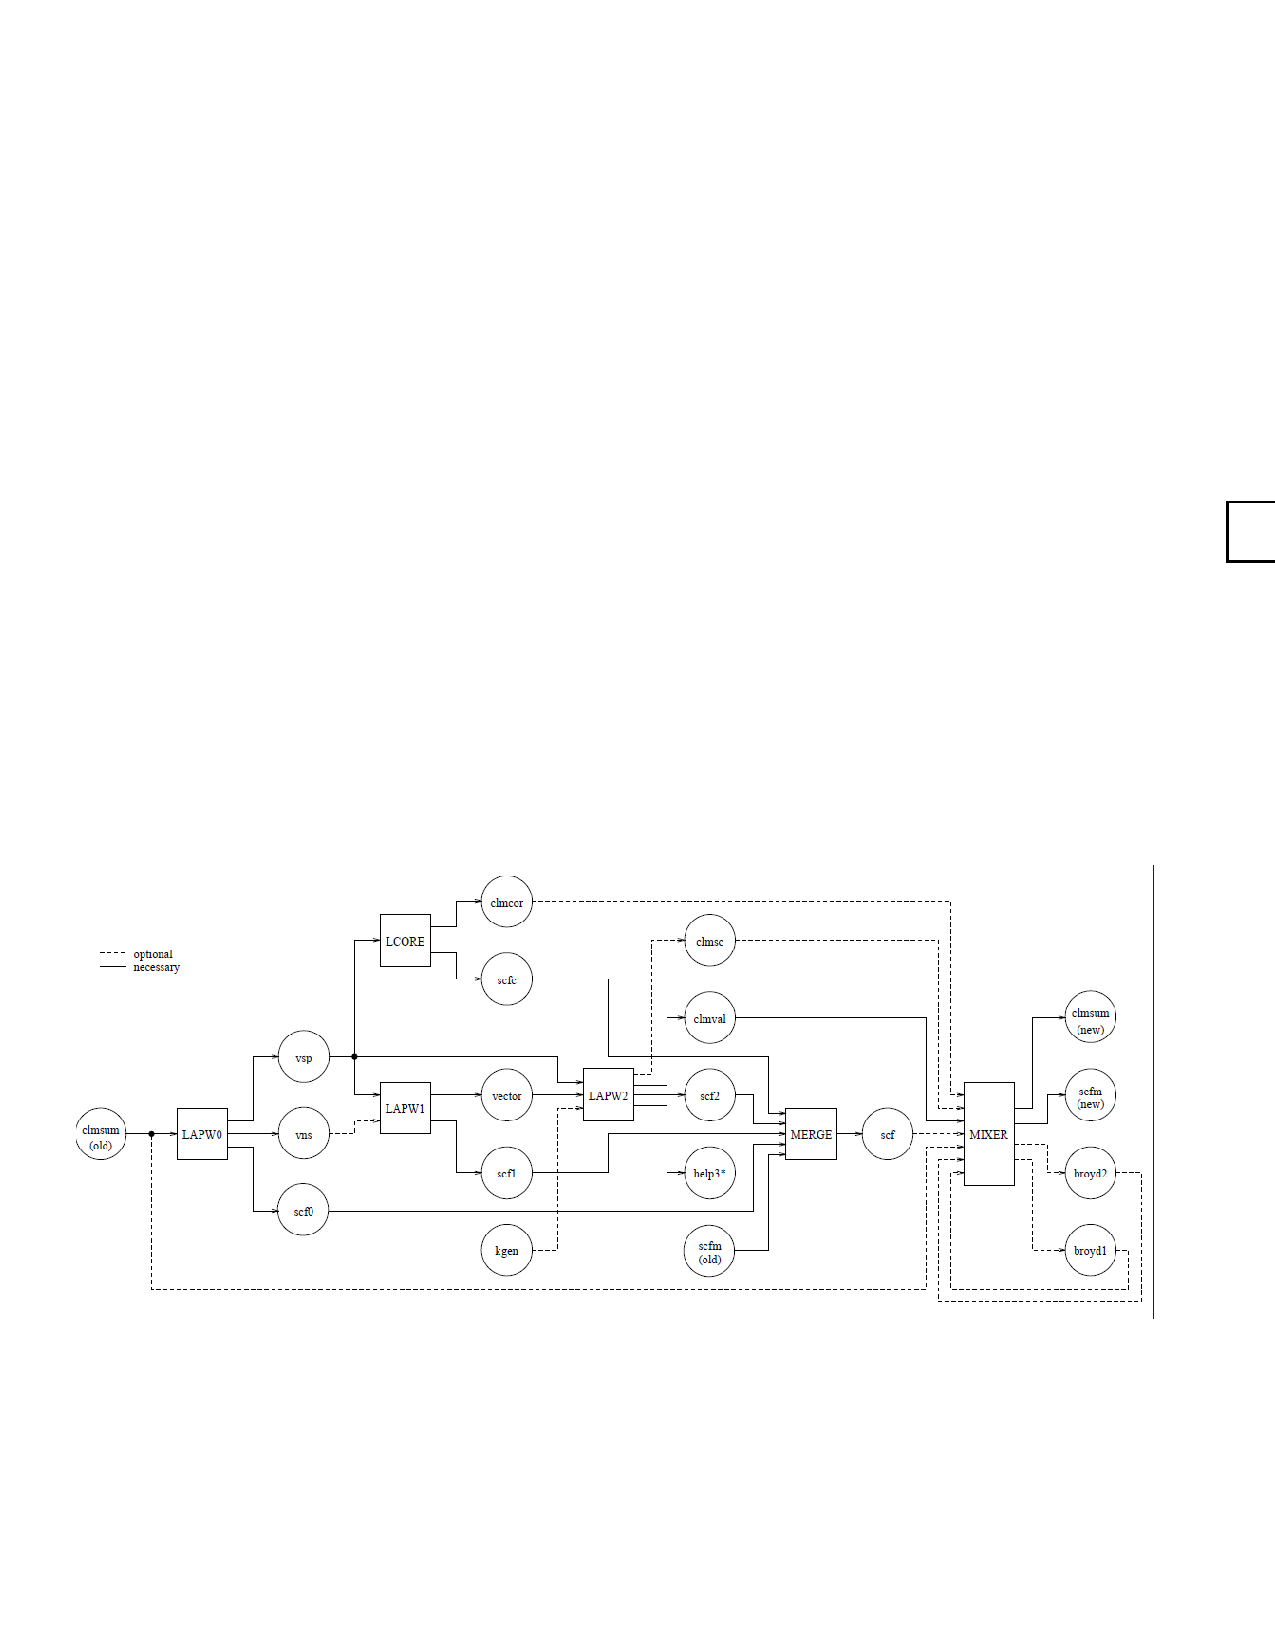
\includegraphics[height=1.72in,width=4.2in,viewport=30 165 550 375,clip]{Figures/WIEN2k_Data_flow.pdf}
\caption{\small \textrm{Data flow during a SCF cycle (programX.def, case.struct, case.inX, case.outputX and optional files are omitted).}}%(与文献\cite{EPJB33-47_2003}图1对比)
\label{WIEN2k_Data_flow}
\end{figure}
}
\frame
{
\frametitle{}
\begin{figure}[h!]
\centering
\vspace*{-20pt}
\includegraphics[height=2.80in,width=1.70in,viewport=60 90 325 500,clip]{Figures/WIEN2k_Program_flow.pdf}
\caption{\small \textrm{Program flow in WIEN2k.}}%(与文献\cite{EPJB33-47_2003}图1对比)
\label{WIEN2k_program_flow}
\end{figure}
}

%\section{PAW方法的基本思想}
%\frame
%{
%\frametitle{PAW方法基本思想}
%\textrm{P. E. Bl\"ochl}尝试了结合赝势方法和\textrm{APW}方法优势的\textrm{(Projected Augmented Wave, PAW)}方法\upcite{PRB50-17953_1994,PRB59-1758_1999}。
%\begin{itemize}
%\setlength{\itemsep}{8pt}
%	\item 与芯层态正交的全部价电子构成的\textrm{Hilbert}空间,价电子彼此的正交使得波函数在\textrm{Muffin-tin}球内振荡
%	\item 作线性变换,将原\textrm{Hilbert}空间变换为赝\textrm{Hilbert}空间,相应的价电子波函数变换为赝波函数
%		$$|\Psi\rangle=\tau|\tilde\Psi\rangle$$
%	\item 赝波函数与全电子波函数在\textrm{Interstitial}区变换前后保持不变,在\textrm{Muffin-tin}球内的波函数变换后可使计算极大的方便\\
%		$$\langle A \rangle=\langle\Psi|\mathrm{A}|\Psi\rangle=\langle\tilde\Psi|\tau^{\dag}\mathrm{A}\tau|\tilde\Psi\rangle=\langle\tilde\Psi|\tilde{\mathrm{A}}|\tilde\Psi\rangle$$
%	$$\tau=1+\sum_{\mathrm R}\hat\tau_{\mathrm R}$$
%	这里每个$\hat\tau_{\mathrm R}$作用的区域是每个原子核附近的\textrm{Muffin-tin}区$\Omega_{\mathrm R}$
%\end{itemize}
%}

%\frame
%{
%\frametitle{PAW方法基本思想}
%$\hat\tau_{\mathrm R}$的定义是在\textrm{Muffin-tin}球区,$\hat\tau_{\mathrm R}$使得赝原子波函数$\tilde\phi_i$与全原子波函数$\phi_i$之间的变换关系满足:
%$$|\phi_i\rangle=(1+\hat\tau_{\mathrm R})|\tilde\phi_i\rangle$$

%在每个\textrm{Muffin-tin}球内,体系的赝波函数用赝原子波函数展开:
%$$|\tilde\Psi\rangle=\sum_i|\tilde\phi_i\rangle c_i$$
%由于$|\phi_i\rangle=\tau|\tilde\phi_i\rangle$,因此\textrm{Muffin-tin}球内全电子波函数可以表示为:
%$$|\Psi\rangle=\tau|\tilde\Psi\rangle=\sum_i|\phi_i\rangle c_i$$
%因此,全电子波函数可以表示为:
%$$|\Psi\rangle=|\tilde\Psi\rangle-\sum_i|\tilde\phi_i\rangle c_i+\sum_i|\phi_i\rangle c_i$$
%}

%\frame
%{
%\frametitle{投影函数及其特征}
%为了确保$\tau$是线性变换,它必须是赝波函数$\tilde\Psi$的线性函数。因此系数$c_i$满足:
%$$c_i=\langle\tilde p_i|\tilde\Psi\rangle$$
%这里$\tilde p_i$称为投影函数\textrm{(projector functions)}。
%投影函数要满足的条件:
%\begin{itemize}
%	\item $$\sum_i|\tilde\phi_i\rangle\langle\tilde p_i|=1$$
%	\item $$\langle\tilde p_i|\tilde\phi_j\rangle=\delta_{ij}$$
%\end{itemize}
%投影函数最一般的形式可以表示为:
%$$\langle\tilde p_i|=\sum_j(\{\langle f_k|\tilde\phi_l\rangle\})_{ij}^{-1}\langle f_j|$$
%这里$|f_j\rangle$组合成一套线性无关的函数。
%}

%\frame
%{
%\frametitle{}
%线性变换算符可以表示为:
%$$\tau=1+\sum_i(|\phi_i\rangle-|\tilde\phi_i\rangle)\langle\tilde p_i|$$
%因此,全电子波函数的表达式为:
%$$|\Psi\rangle=|\tilde\Psi\rangle+\sum_i(|\phi_i\rangle-|\tilde\phi_i\rangle)\langle\tilde p_i|\tilde\Psi\rangle$$

%对于芯层态$|\Psi^c\rangle$,处理与价层态类似:
%$$|\Psi^c\rangle=|\tilde\Psi^c\rangle+|\phi^c\rangle-|\tilde\phi^c\rangle$$
%但芯层态不需要定义相应的投影函数,本质上是冻芯近似的处理方式。
%}

%\frame
%{
%\frametitle{PAW方法的算符和密度表示}
%因为引入变换算符$\tau$,波函数由\textrm{Schr\"odinger}表象变为\textrm{Heisenberg}表象。因此在赝波函数构成的\textrm{Hilbert}空间内,算符的变换满足:
%\begin{displaymath}
%\begin{aligned}
%	\tilde A &=\tau^{\dag}A\tau \\
%			&=A+\sum_{i,j}|\tilde p_i\rangle(\langle\phi_i|A|\phi_j\rangle-\langle\tilde\phi_i|A|\tilde\phi_j\rangle)\langle\tilde p_j|
%\end{aligned}
%\end{displaymath}
%由此,可以得到电荷密度的表达式为:
%$$n(\vec r)=\tilde n(\vec r)+n^1(\vec r)-\tilde n^1(\vec r)$$
%\footnotesize{
%这里
%$$\tilde n(\vec r)=\sum_nf_n\langle\tilde\Psi_n|\vec r\rangle\langle\vec r|\tilde\Psi_n\rangle$$
%$$n^1(\vec r)=\sum_{n,(i,j)}f_n\langle\tilde\Psi_n|\tilde p_i\rangle\langle\phi_i|\vec r\rangle\langle\vec r|\phi_j\rangle\langle\tilde p_j|\tilde\Psi_n\rangle$$
%$$\tilde n^1(\vec r)=\sum_{n,(i,j)}f_n\langle\tilde\Psi_n|\tilde p_i\rangle\langle\tilde\phi_i|\vec r\rangle\langle\vec r|\tilde\phi_j\rangle\langle\tilde p_j|\tilde\Psi_n\rangle$$
%}}

%\frame
%{
%	\frametitle{总能量的表示}
%总能量泛函
%\begin{displaymath}
%	\begin{aligned}
%		E&=\sum_nf_n\langle\Psi_n|-\dfrac12\nabla^2|\Psi_n\rangle\\
%		 &+\dfrac12\int\mathrm{d}\vec r\int\mathrm{d}\vec r^{\prime}\dfrac{(n+n^Z)(n+n^Z)}{|\vec r-\vec r^{\prime}|}+\int\mathrm{d}\vec r n\epsilon_{\mathrm{XC}}(n)
%	\end{aligned}
%\end{displaymath}
%与密度表达式类似,$E=\tilde E+E^1-\tilde E^1$,每一项分别表示为:
%\footnotesize{
%\begin{displaymath}
%	\begin{aligned}
%		\tilde E&=\sum_nf_n\langle\tilde\Psi_n|-\dfrac12\nabla^2|\tilde\Psi_n\rangle\\
%		 &+\dfrac12\int\mathrm{d}\vec r\int\mathrm{d}\vec r^{\prime}\dfrac{(\tilde n+\hat n)(\tilde n+\hat n)}{|\vec r-\vec r^{\prime}|}+\int\mathrm{d}\vec r \tilde n\bar v+\int\mathrm{d}\vec r \tilde n\epsilon_{\mathrm{XC}}(\tilde n)
%	\end{aligned}
%\end{displaymath}
%\begin{displaymath}
%	\begin{aligned}
%		E^1&=\sum_{n,(i,j)}f_n\langle\tilde\Psi_n|\tilde p_i\rangle\langle\phi_i-\dfrac12\nabla^2|\phi_j\rangle\tilde p_j\tilde\Psi_n\rangle\\
%		 &+\dfrac12\int\mathrm{d}\vec r\int\mathrm{d}\vec r^{\prime}\dfrac{(n^1+n^Z)(n^1+n^Z)}{|\vec r-\vec r^{\prime}|}+\int\mathrm{d}\vec r n^1\epsilon_{\mathrm{XC}}(n^1)
%	\end{aligned}
%\end{displaymath}
%\begin{displaymath}
%	\begin{aligned}
%		\tilde E^1&=\sum_{n,(i,j)}f_n\langle\tilde\Psi_n|\tilde p_i\rangle\langle\tilde\phi_i-\dfrac12\nabla^2|\tilde\phi_j\rangle\tilde p_j\tilde\Psi_n\rangle\\
%		 &+\dfrac12\int\mathrm{d}\vec r\int\mathrm{d}\vec r^{\prime}\dfrac{(\tilde n^1+\hat n)(\tilde n^1+\hat n)}{|\vec r-\vec r^{\prime}|}+\int\mathrm{d}\vec r \tilde n^1\bar v+\int\mathrm{d}\vec r \hat n^1\epsilon_{\mathrm{XC}}(\hat n^1)
%	\end{aligned}
%\end{displaymath}
%}}

%\frame
%{
%	\frametitle{补偿电荷密度$\hat n$的计算}
%$n^Z$表示原子核位置的点电荷密度,$\hat n$称为补偿电荷密度。\\
%$\hat n$的作用:\large{\bf 使$(n^1+n^Z)$与$(\hat n^1+\hat n)$具有相同的多极矩展开},并且$\hat n=\sum\nolimits_R\hat n_R$,在每个\textrm{Muffin-tin}球内:
%$$\hat n_R(r)=\sum_Lg_{RL}(r)Q_{RL}$$
%其中
%$$g_{RL}(r)=C_l|\vec r-\vec R|^lY_L(r-R)\mathrm{e}^{-(|\vec r-\vec R|/r_c)^2}$$
%$$Q_{RL}=\int\mathrm{d}\vec r|\vec r-\vec R|^l[n^1_R(\vec r)+n^Z_R(\vec r)-\tilde n^1_R(\vec r)]Y^{\ast}_L(\vec r-\vec R)$$
%如果直接计算$\hat n_R(r)$,\textrm{Gaussian}函数非常尖锐。实际计算时引入赝补偿电荷$\hat n^{\prime}$,它与$\hat n$具有相同的多极矩展开,但相应的级数$g^{\prime}_{RL}(r)$平缓得多。
%}

%\frame
%{
%	\frametitle{}
%因此$\tilde E$中的静电相互作用的表达式为:
%\begin{displaymath}
%	\begin{aligned}
%		&\dfrac12\int\mathrm{d}\vec r\int\mathrm{d}\vec r^{\prime}\dfrac{(\tilde n+\hat n)(\tilde n+\hat n)}{|\vec r-\vec r^{\prime}|}\\
%	=&\dfrac12\int\mathrm{d}\vec r\int\mathrm{d}\vec r^{\prime}\dfrac{(\tilde n+\hat n^{\prime})(\tilde n+\hat n^{\prime})}{|\vec r-\vec r^{\prime}|}\\
%		&+\int\mathrm{d}\vec r\int\mathrm{d}\vec r^{\prime}\tilde n(\vec r)\dfrac{\hat n(\vec r^{\prime})-\hat n^{\prime}(\vec r^{\prime})}{|\vec r-\vec r^{\prime}|}\\
%		&+\sum_{\vec R,\vec R^{\prime}}\dfrac12\int\mathrm{d}\vec r\int\mathrm{d}\vec r^{\prime}\dfrac{\hat n_R(\vec r)\hat n_{R^{\prime}}(\vec r^{\prime})-\hat n^{\prime}_R(\vec r)\hat n^{\prime}_{R^{\prime}}(\vec r^{\prime})}{|\vec r-\vec r^{\prime}|}
%	\end{aligned}
%\end{displaymath}
%}

%\frame
%{
%	\frametitle{PAW方法的重叠算符和Hamilton算符}
%重叠算符:
%$$\tilde O=1+\sum_{i,j}|\tilde p_i\rangle[\langle\phi_i|\phi_j\rangle-\langle\tilde\phi_i|\tilde\phi_j\rangle]\langle\tilde p_j|$$
%\textrm{Hamiliton}算符
%\begin{itemize}
%	\item 动能算符:
%		$$\tilde T=-\dfrac12\nabla^2+\sum_{i,j}|\tilde p_i\rangle[\langle\phi_i|-\dfrac12\nabla^2|\phi_j\rangle-\langle\tilde\phi_i|-\dfrac12\nabla^2|\tilde\phi_j\rangle]\langle\tilde p_j|$$
%	\item 完全势\textrm{(full-potential)}算符:
%$$v(\vec r)=\tilde v(\vec r)+v^1(\vec r)-\tilde v^1(\vec r)$$
%	\item \textrm{Hamilton}算符:
%		$$\tilde H=-\dfrac12\nabla^2+\tilde v+\sum_{i,j}|\tilde p_i\rangle[\langle\phi_i|-\dfrac12\nabla^2+v^1|\phi_j\rangle-\langle\tilde\phi_i|-\dfrac12\nabla^2+\tilde v^1|\tilde\phi_j\rangle]\langle\tilde p_j|$$
%\end{itemize}
%}

%\frame
%{
%	\frametitle{分波函数$\phi_i$的构造}
%	\begin{itemize}
%		\item 全电子分波函数由方程:
%			$$\biggl(\dfrac12\nabla^2+v_{at}-\epsilon_i^1\biggr)|\phi_i\rangle=0$$
%			计算得到
%		\item 赝势分波函数由方程:
%			$$\biggl(\dfrac12\nabla^2+w_{i}(\vec r)-\epsilon_i^1\biggr)|\tilde\phi_i\rangle=0$$
%			计算得到。\\
%			这里$w_i(\vec r)=\tilde v_{at}(\vec r)+c_ik(\vec r)$,由赝势$\tilde v_{at}(\vec r)$确定。\\
%		\item 赝势$\tilde v_{at}(\vec r)$的确定:对不含\textit{d}电子体系与过渡元素体系采用不同的形式。
%		\end{itemize}
%}

%\frame
%{
%	\frametitle{投影函数$\tilde p_i$的构造}
%	\begin{itemize}
%		\item $\tilde p_i$由递推方式得到,初始的$\tilde p_i$的生成:
%			$$|\tilde p_i\rangle=\biggl(\dfrac12\nabla^2+\tilde v_{at}-\epsilon_i^1\biggr)|\tilde\phi_i\rangle$$
%		\item 根据正交关系$\langle\tilde p_i|\tilde\phi_j\rangle=\delta_{ij}$有:
%			$$|\tilde p_i\rangle=|\tilde p_i\rangle-\sum_{j=1}^{i-1}|\tilde p_j\rangle\langle\tilde\phi_j|\tilde p_i\rangle$$
%		为确保分波函数与投影函数正交:
%			$$|\phi_i\rangle=|\phi_i\rangle-\sum_{j=1}^{i-1}|\phi_j\rangle\langle\tilde p_j|\tilde\phi_i\rangle$$
%			$$|\tilde\phi_i\rangle=|\tilde\phi_i\rangle-\sum_{j=1}^{i-1}|\tilde\phi_j\rangle\langle p_j|\tilde\phi_i\rangle$$
%		\end{itemize}
%}
%\frame
%{
%\frametitle{}
%		最终的投影函数和分波函数的表达式为:
%			$$|\tilde p_i\rangle=|\tilde p_i\rangle/\langle\tilde p_i|\tilde\phi_i\rangle\times c$$
%			$$|\tilde\phi_i\rangle=|\tilde\phi_i\rangle/c$$
%			$$|\phi_i\rangle=|\phi_i\rangle/c$$
%			$c$是为防止数值误差引入的常数。
%}

%\frame
%{
%\frametitle{PAW方法和US-PP方法}
%\begin{itemize}
%\setlength{\itemsep}{15pt}
%	\item \textrm{PAW}方法在\textrm{Muffin-tin}球内使用的是原子真实势和全电子波函数
%	\item \textrm{PAW}方法提供了体系全电子波函数与赝波函数之间的变换关系
%	\item 赝势方法计算重叠矩阵和电荷密度依赖于所构造赝势的散射性质,\textrm{PAW}方法则利用赝电荷多极矩方式更合理地实现
%	\item 因为\textrm{PAW}方法使用原子径向函数,平面波截断大大降低,比传统的赝势方法计算效率更高
%	\end{itemize}
%}

%\frame
%{
%\frametitle{PAW方法和LAPW方法}
%\begin{itemize}
%	\item \textrm{LAPW}基函数为了保持\textrm{Muffin-tin}球和\textrm{Interstitial}区的函数衔接,球内部分函数要展开到足够高阶,\textrm{PAW}方法的原子波函数展开的阶数要低很多
%	\item \textrm{PAW}方法是更一般的方法,\textrm{LAPW}方法可以视为\textrm{PAW}方法的一种特例:
%		$$|\Psi\rangle=(1-\theta_{\Omega_R})|\tilde\Psi\rangle+\theta_{\Omega_R}(|\phi_{\nu}\rangle a-|\phi_{\nu}\rangle b)$$
%		这里系数$a$、$b$满足
%		\begin{displaymath}
%			\biggl[
%			\begin{aligned}
%				a\\b
%			\end{aligned}\biggr]=\dfrac1{(\phi_{\nu}\partial_r\dot\phi_{\nu}-\dot\phi_{\nu}\partial_r\phi_{\nu})}\biggl[
%			\begin{aligned}
%				\tilde\Psi\partial_r\dot\phi_{\nu}\quad&-\dot\phi_{\nu}\partial_r\tilde\Psi\\
%				\phi_{\nu}\partial_r\tilde\Psi\quad&-\tilde\Psi\partial_r\phi_{\nu}
%			\end{aligned}
%			\biggr]
%		\end{displaymath}
%		据此,相应的\textrm{PAW}方法的投影函数可以构造为$$|\tilde p_i\rangle=\sum_j(\nabla^2\theta_{\Omega_R})|\tilde\phi_j\rangle c_{ji}$$
%		系数$c_{ij}$由正交条件$\langle p_i|\phi_j\rangle=\delta_{ij}$确定。
%	\end{itemize}
%}

\section{$\vec k$空间积分与布点}
\frame
{
\frametitle{能带、\textrm{Fermi}面与$\vec k$空间积分}
\vspace{30pt}
\begin{figure}[h!]
\centering
\hspace*{-0.30in}
\subfigure[\textrm{Band structure}]{
\label{Band_Gap_Fermi-1}
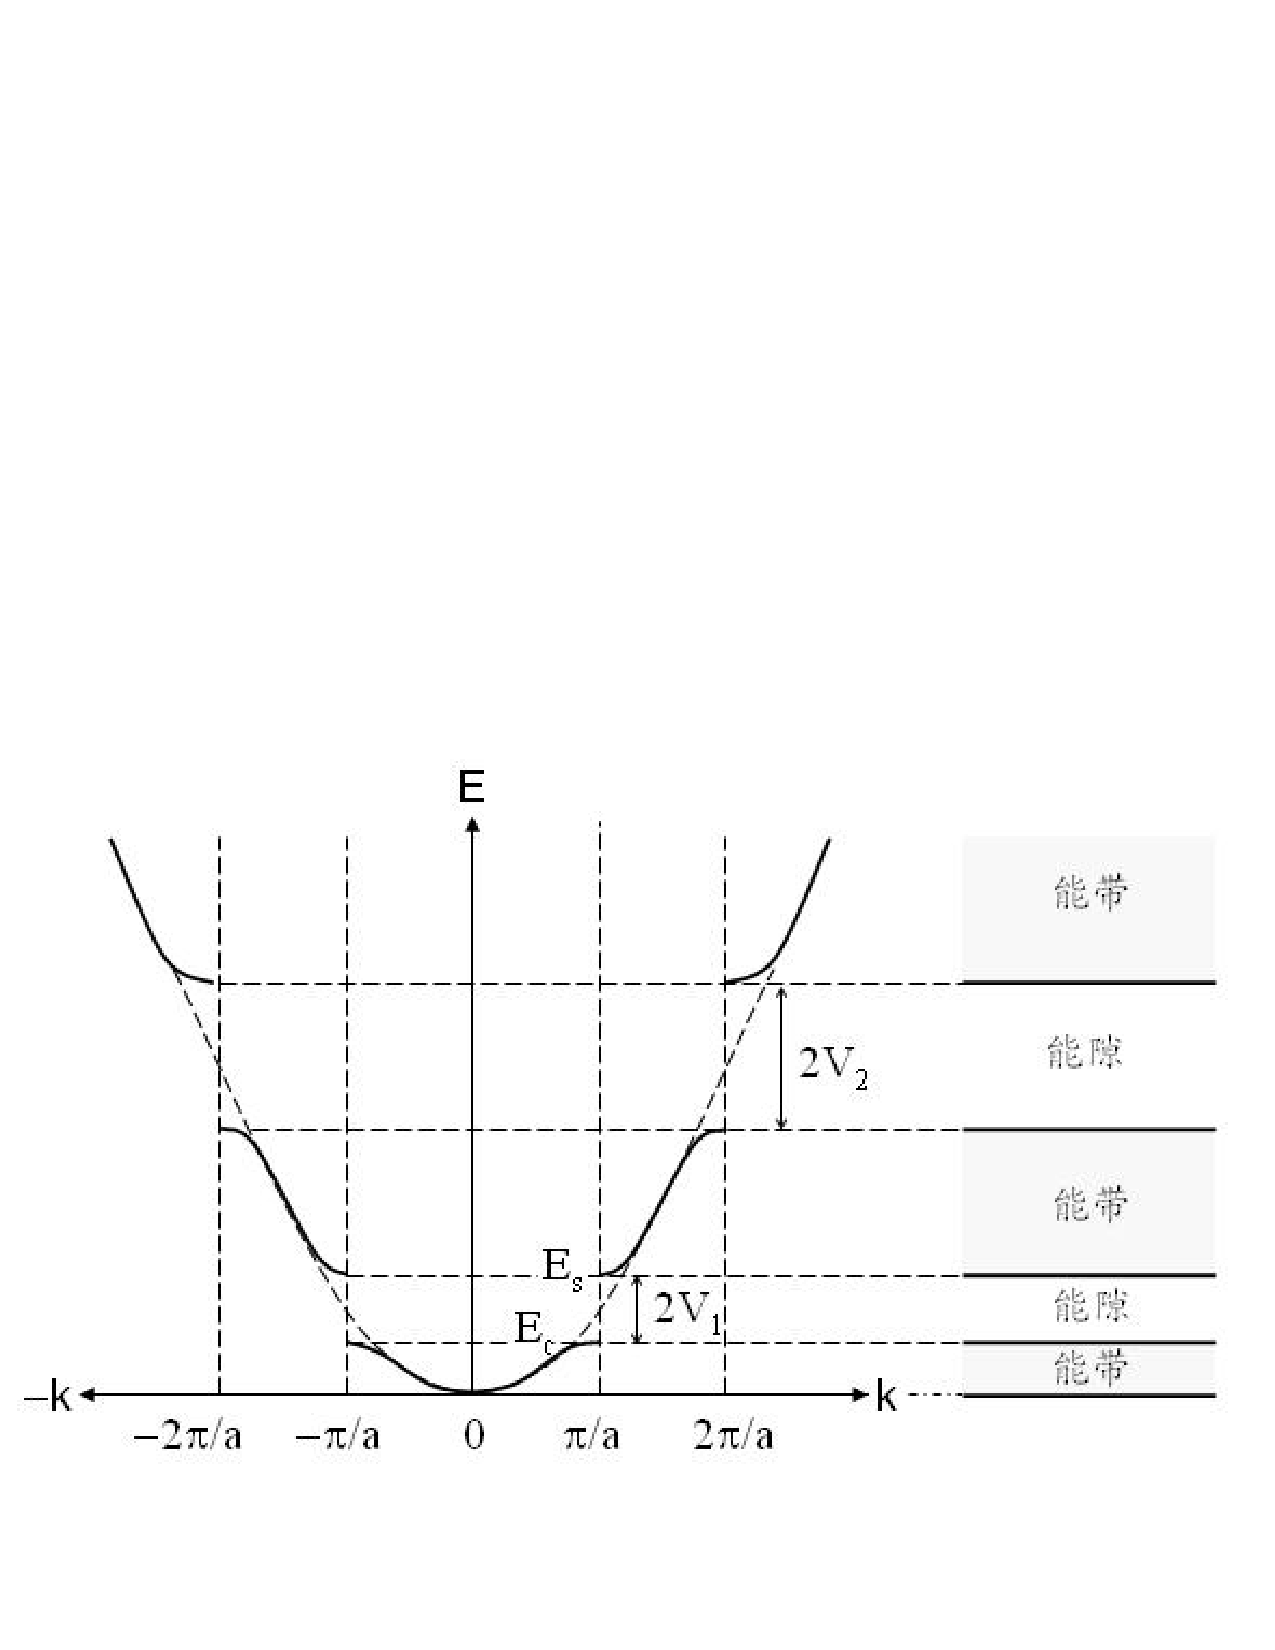
\includegraphics[height=1.3in,width=2.3in,viewport=10 90 570 380,clip]{Figures/Band_Gap.pdf}}
\subfigure[\textrm{Brillouin Zone}]{
\label{Band_Gap_Fermi-2}
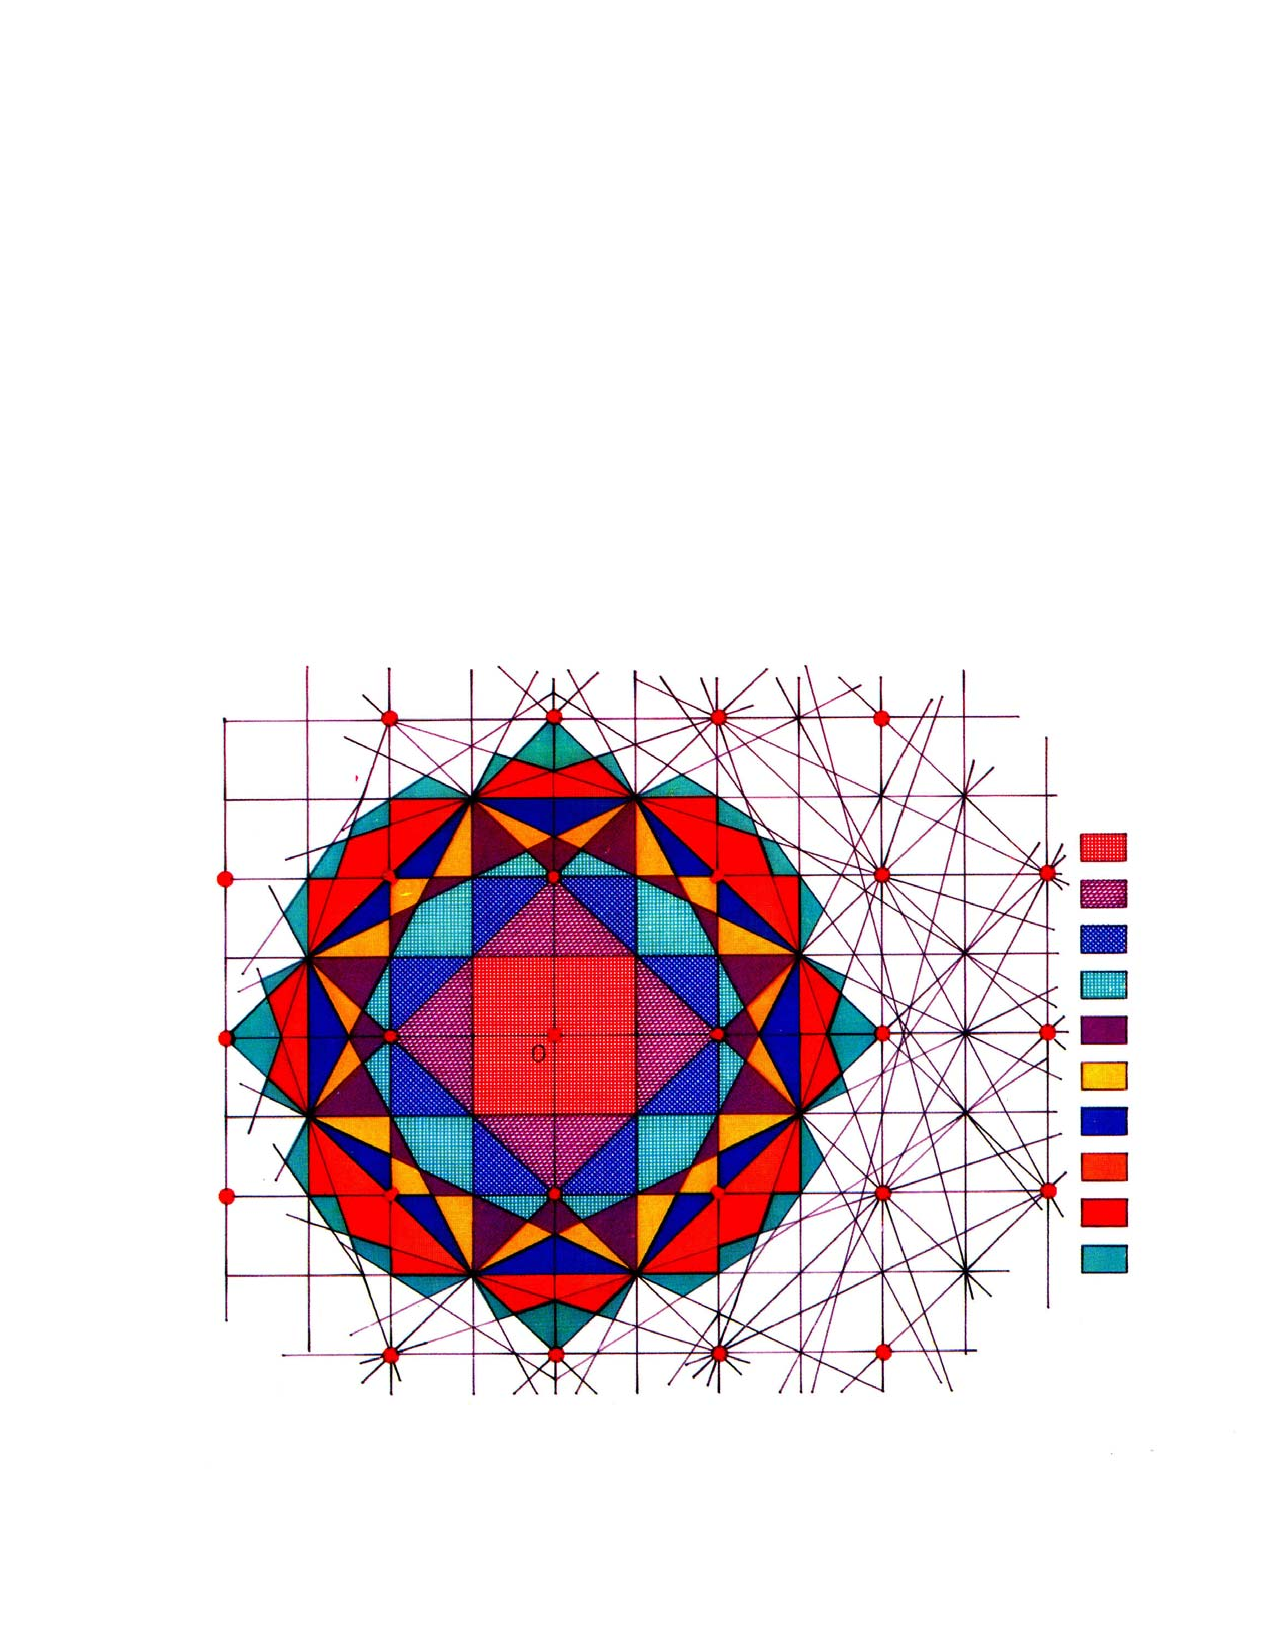
\includegraphics[height=1.28in,width=1.75in,viewport=100 120 545 470,clip]{Figures/2D_Brillouin-Zone.pdf}}
\label{Band_Gap_Fermi}
\end{figure}
}

\frame
{
\frametitle{$\vec k$ 空间布点方案}
\vskip 10pt
周期性体系计算,涉及除了在每个格点上求解\textrm{Schr\"odinger}方程外,\\计算固体性质的时还需要对$\vec k$空间中完成数值积分。
%\textbf{期望值},$\vec k$空间布点数值测试
\vskip 5pt
\begin{itemize}%[+-| alert@+>]
%\begin{enumerate}%[+-| alert@+>]
%\item $\vec k$空间布点方案
%  \begin{enumerate}
%\setlength{\itemsep}{15pt}
    \item 特殊点布点方案\textrm{(spectial points method)}\\
      将\textrm{Brillouin}区的积分变成网格点的权重求和
    \item 四面体布点方案\textrm{(tetrahedron method)}\upcite{PRB49-16233_1994}\\
	    \textrm{Brillouin}区积分转换为对网格点构成的四面体求和
%  \end{enumerate}
\end{itemize}
\begin{figure}[h!]
\centering
\vspace*{-0.2in}
\subfigure[\textrm{Special points}]{
\label{Special_Points-1}
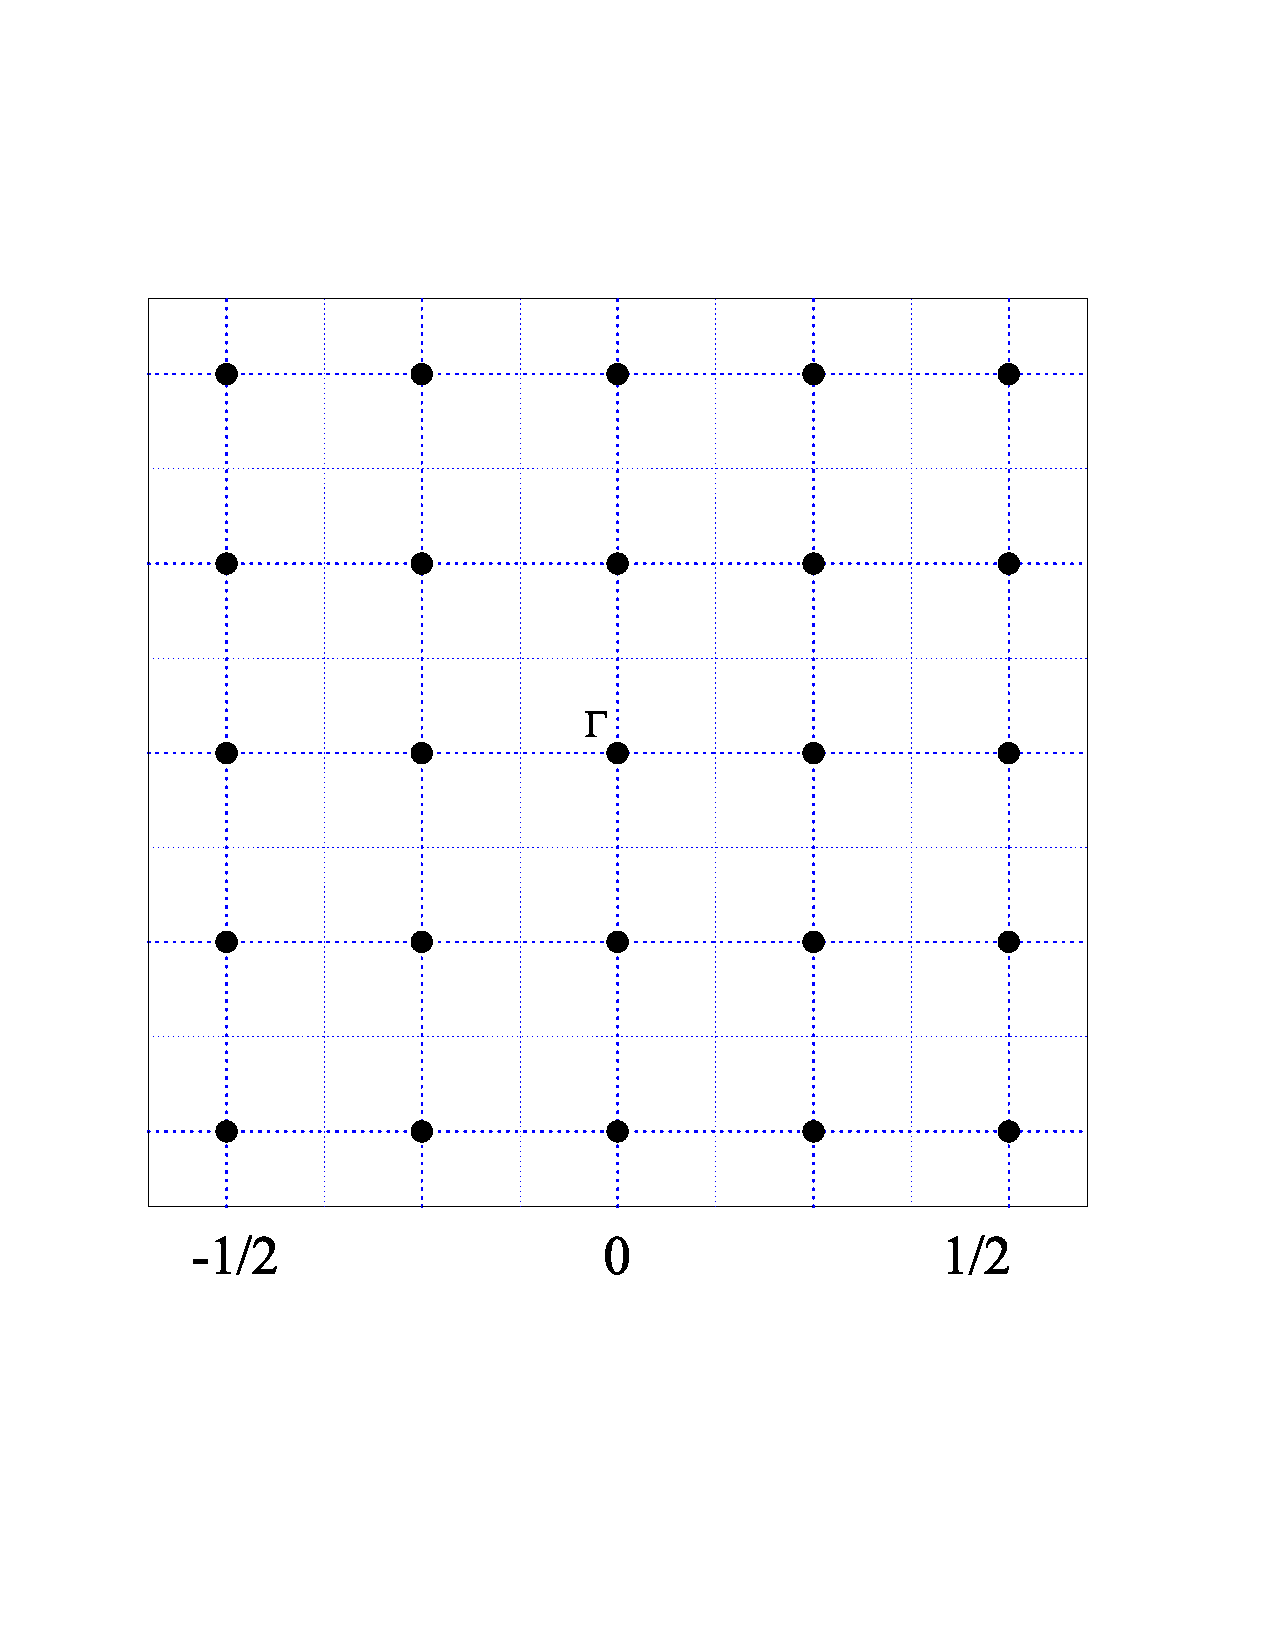
\includegraphics[height=1.28in,width=1.24in,viewport=65 175 525 650,clip]{Figures/Special-points-1.pdf}}
\subfigure[\textrm{Tetrahedron}]{
\label{Tetrahedron-2}
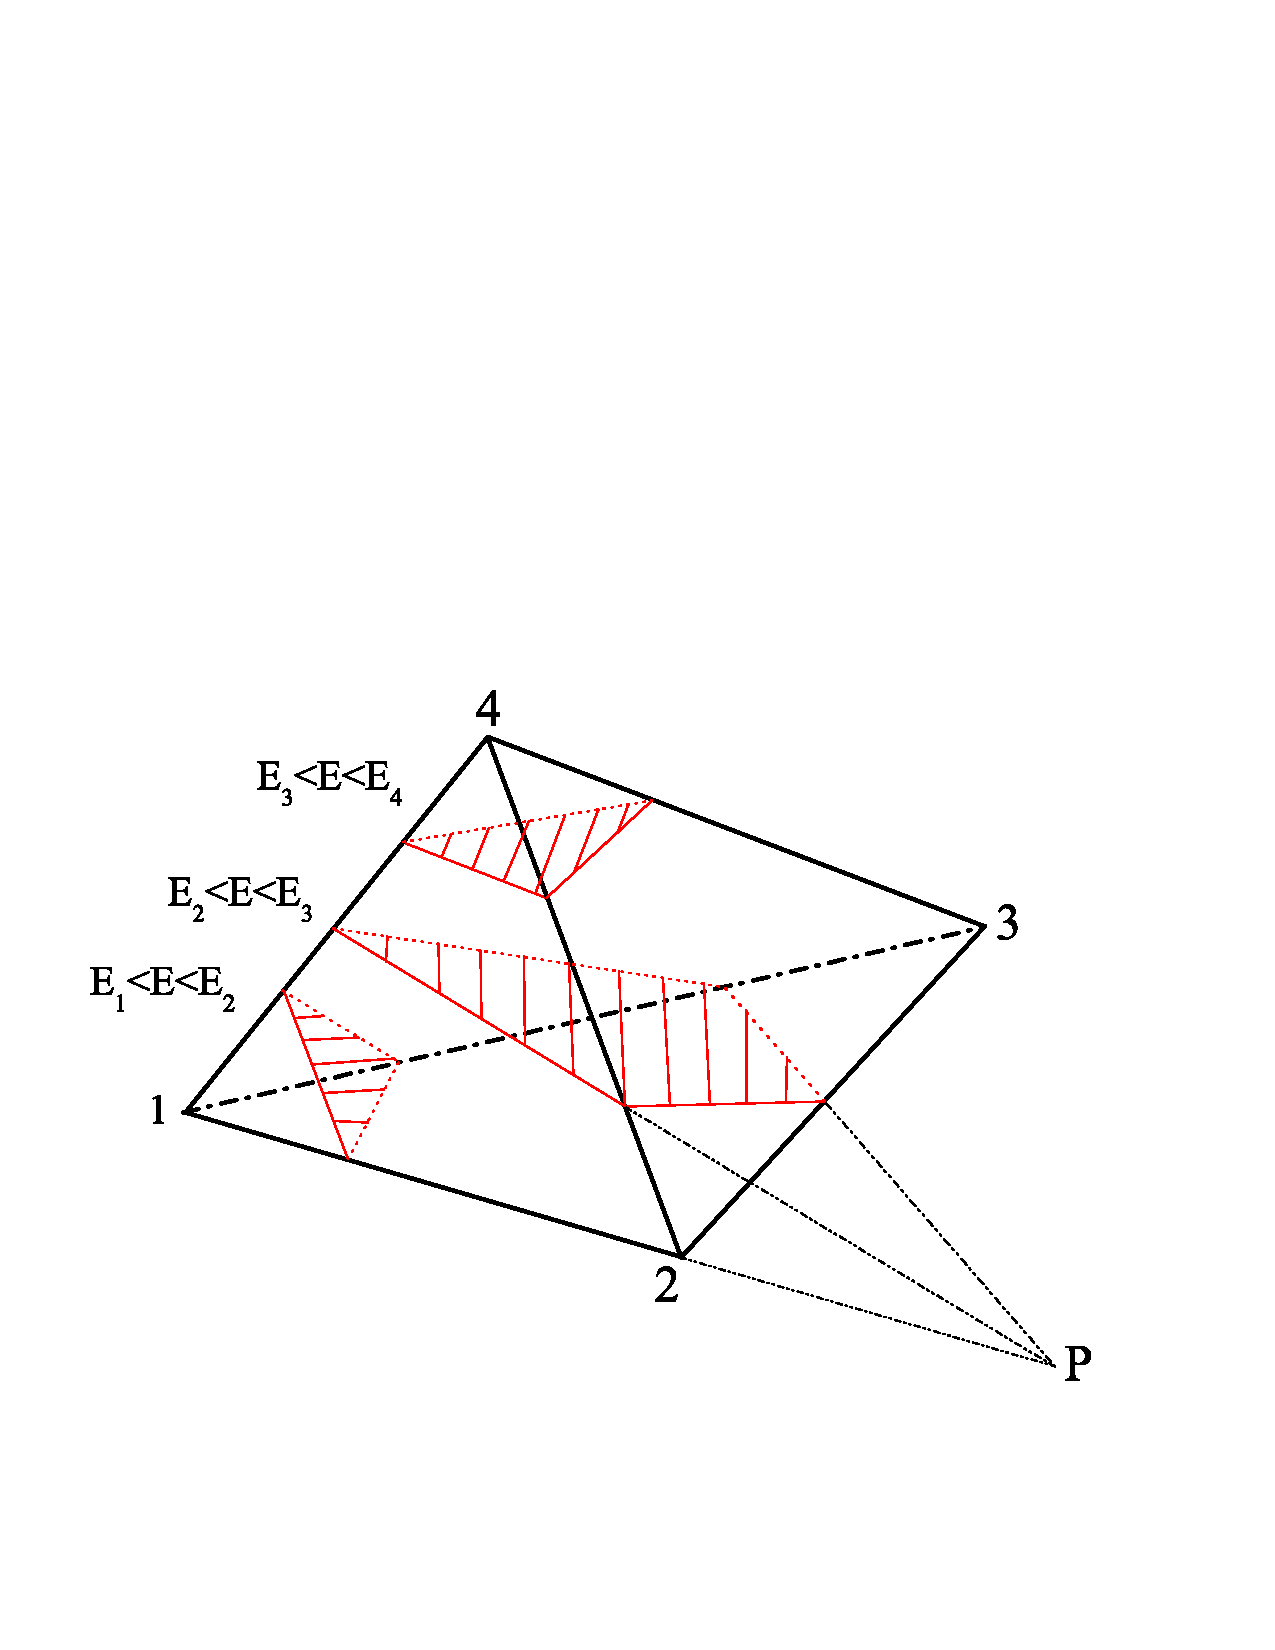
\includegraphics[height=1.28in,width=1.75in,viewport=40 125 525 465,clip]{Figures/Tetra-equal-ene.pdf}}
\label{Specila_Tetrahedron}
\end{figure}
}

\frame
{
\frametitle{四面体布点积分方案}
\begin{itemize}
\setlength{\itemsep}{5pt}
	\item 对\textrm{WS}元胞用$N=(N_1+1)\times(N_2+1)\times(N_3+1)$个\\网格点(依次编号)分割为$N_1\times N_2\times N_3$个平行六面体
	\item 将每个平行六面体分为4个四面体,记下四面体顶点编号
\end{itemize}
\begin{figure}[h!]
\centering
\hspace*{-10pt}
\vspace*{-10pt}
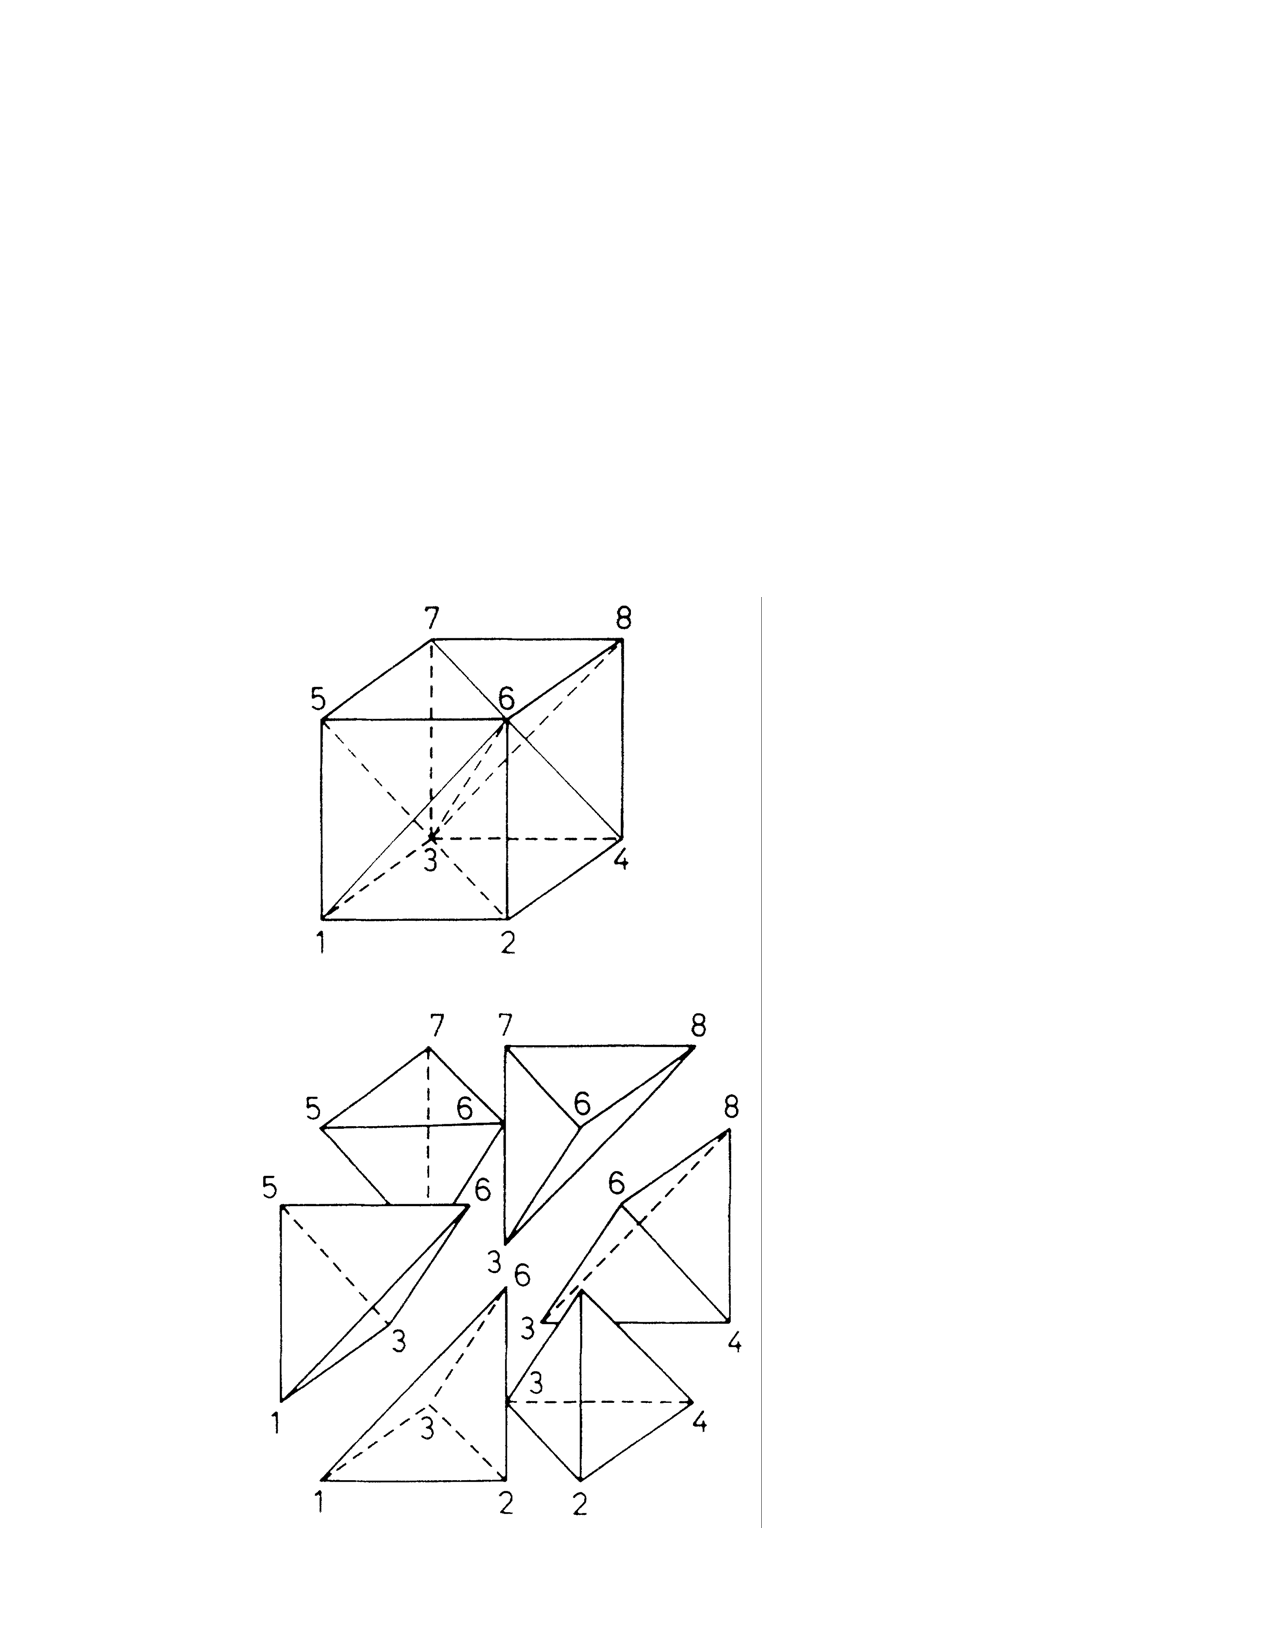
\includegraphics[height=1.8in,width=1.05in,viewport=120 60 360 505,clip]{Figures/submesh_Tetra.pdf}
\caption{\small \textrm{Breakup of a submesh cell into six tetrahedra.}}%(与文献\cite{EPJB33-47_2003}图1对比)
\label{Tetrahedron_split}
\end{figure}
}

\frame
{
\frametitle{四面体布点积分方案}
\begin{itemize}
\setlength{\itemsep}{10pt}
	\item 用点群对称性操作遍历全部网格点,各点对应的不可约第一\\\textrm{Brillouin}区\textrm{(Irreducible Brillouin zone, IBZ)}等价点标记
	\item 记录不可约\textrm{IBZ}的$\vec k$点及其权重
	\item 四面体中顶点编号全同的归为一类,同时统计各类四面体\\顶点序号和数目
\end{itemize}
每个四面体对$\vec k$-空间积分的权重表达式可参阅文献\cite{PRB49-16233_1994}
\begin{figure}[h!]
\centering
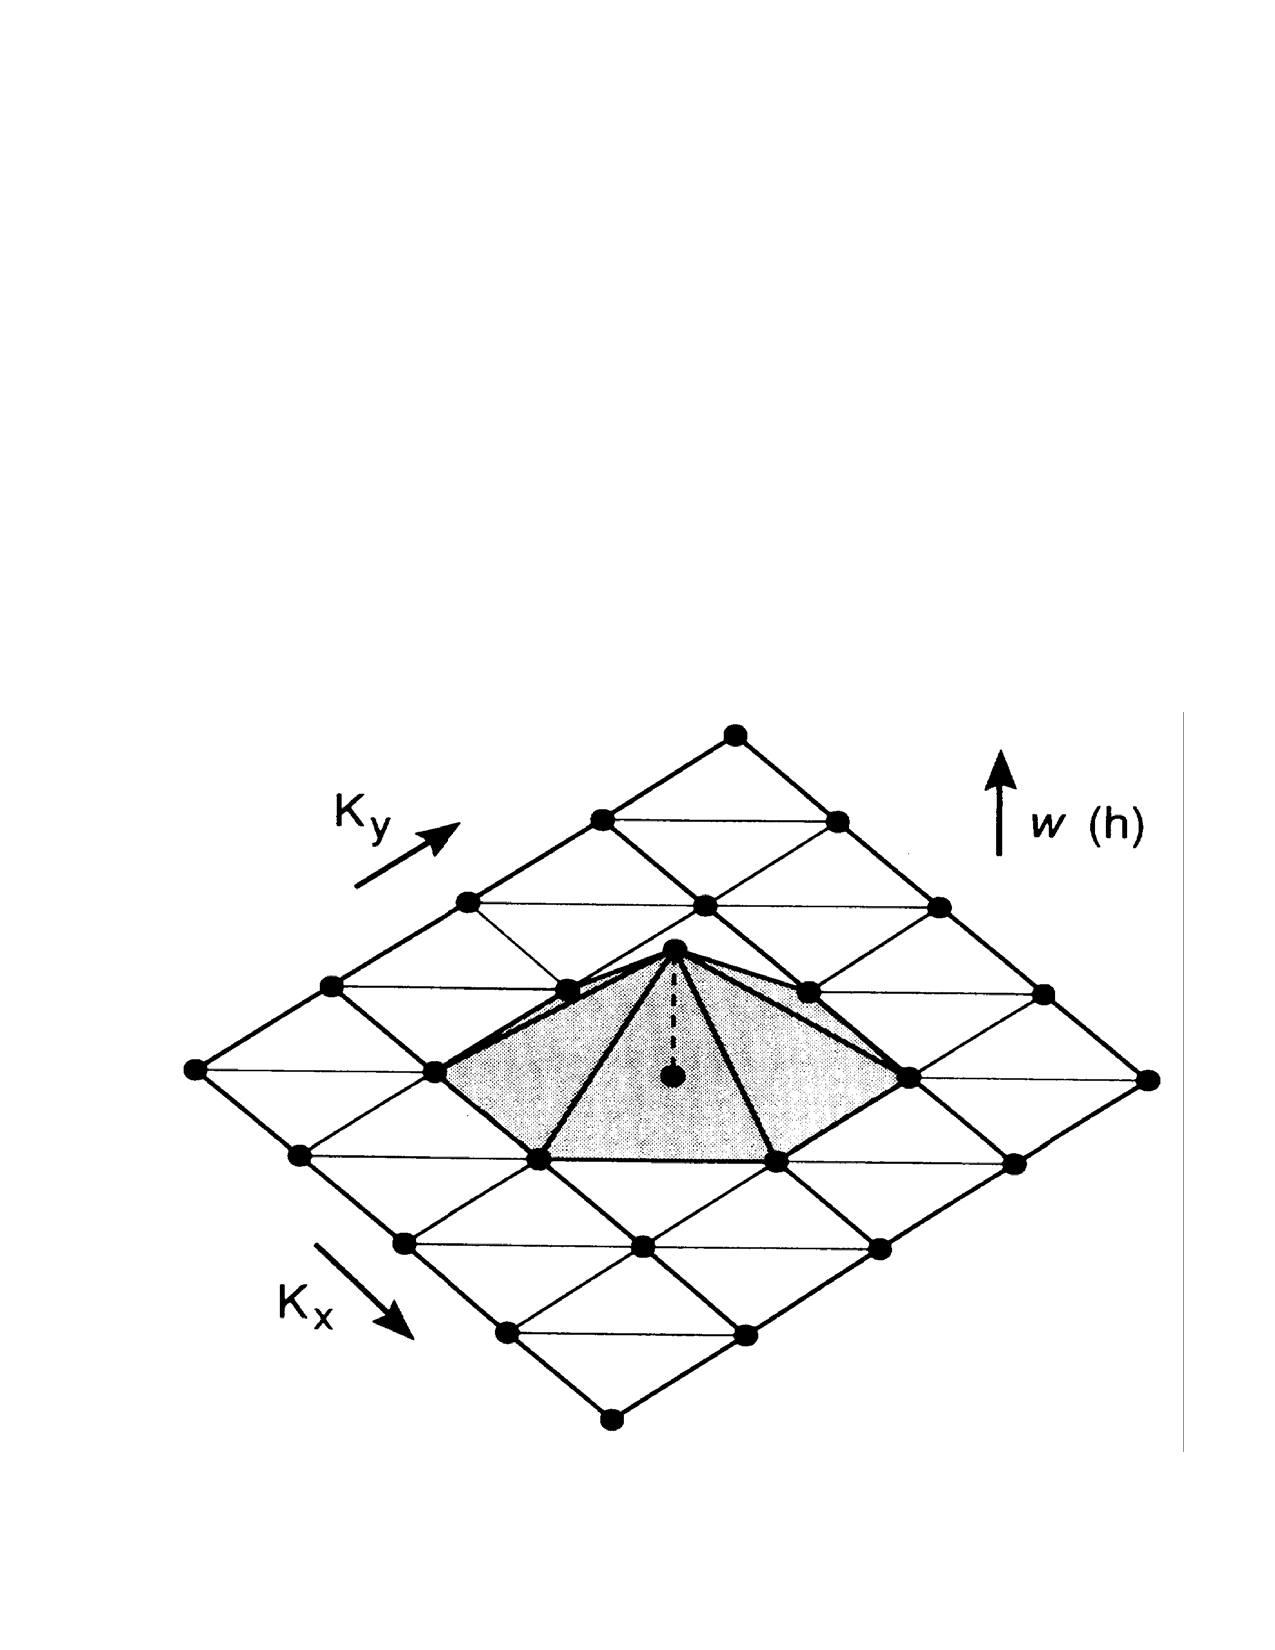
\includegraphics[height=0.95in,width=1.32in,viewport=85 99 560 460,clip]{Figures/dimen_Tetra.pdf}
\caption{\small \textrm{Two-dimensional schematic illustration of the functions $w_j(\vec k)$ that result in the integration weights when integrated.}}%(与文献\cite{EPJB33-47_2003}图1对比)
\label{Tetrahedron_weight}
\end{figure}
}

\frame
{
\frametitle{四面体布点积分方案}
\begin{figure}
\centering
\begin{minipage}[b]{0.45\linewidth}
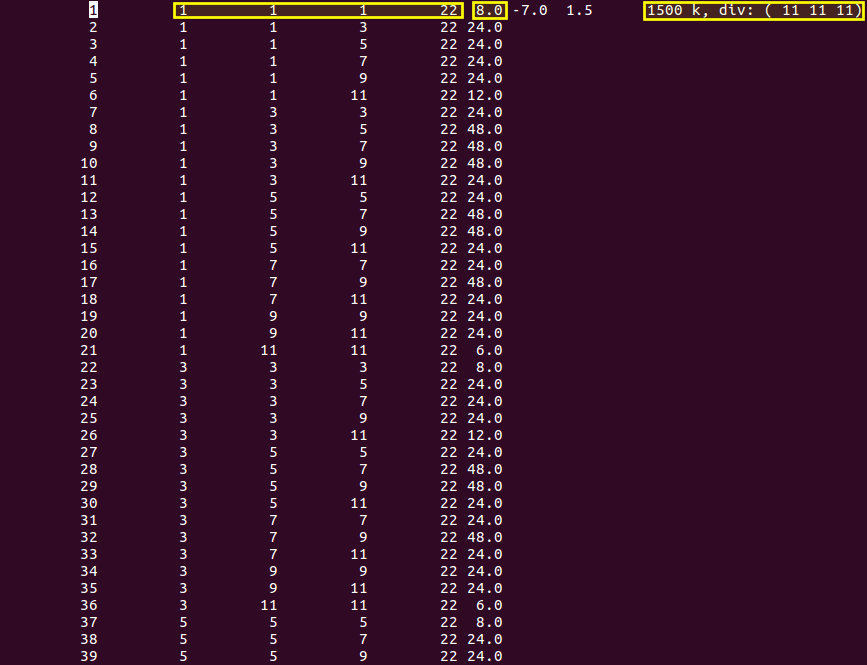
\includegraphics[height=0.65\textheight,width=1.07\textwidth,viewport=70 0 900 700,clip]{Figures/WIEN2k_CaB6-klist.png}
\caption{\small{\textrm{case.klist}}}
\end{minipage}
\begin{minipage}[b]{0.45\linewidth}
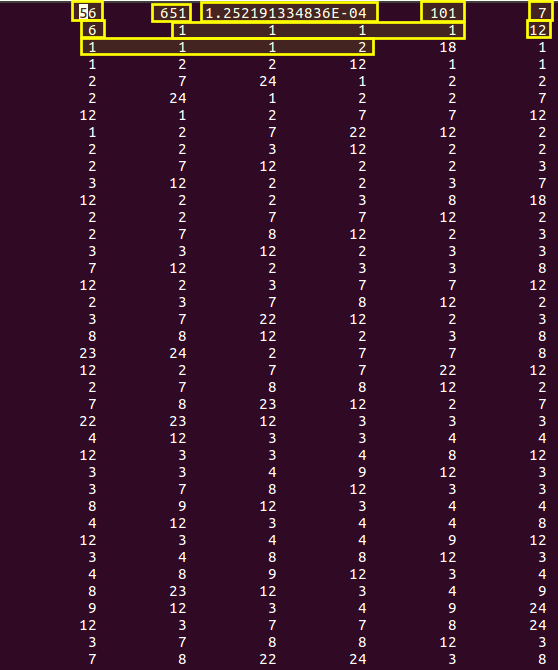
\includegraphics[height=0.65\textheight,width=1.0\textwidth,viewport=0 0 670 700,clip]{Figures/WIEN2k_CaB6-kgen.png}
\caption{\small\textrm{case.kgen}}
\end{minipage}
\end{figure}
}

\section{LDA+U与自相互作用的校正}
\frame
{
\frametitle{LDA+$U$校正的基本思想}
\begin{itemize}
\setlength{\itemsep}{10pt}
	\item 精确密度泛函具有当电子数在整数值前后改变的时候,体系能量的改变是不连续的属性,单电子能量的不连续对能带的带隙有很大贡献
	 \item\textrm{LDA~}近似中体系能量是电子数的连续函数,不具备体系能量随电子数变化不连续的特征。\textrm{LDA/GGA~}方法在描述含有$d$/$f$电子的过渡金属和稀土元素化合物体系时常常失效。
	\item \textrm{LDA}/\textrm{GGA~}得到的体系总能量和实验结果符合较好,但轨道能量(即$\varepsilon_i=\partial E/\partial n_i$),不符合\textrm{Koopmans~}定理,与实验或者严格计算得到的轨道能量差别很大%一个典型的例子就是对H原子的计算结果,LDA计算的轨道能级为$-$0.27\,a.u.(实验结果为$-$0.5\,a.u.),总能量($-$0.488\,a.u.)则非常接近$-$0.5\,a.u.\upcite{PRB37-9919_1988}。
	\item \textrm{Anisimov~}提出通过对\textrm{LDA~}势加入轨道校正克服不足(称为\textrm{LDA+$U$}方法)\upcite{PRB44-943_1991,PRB48-16929_1993}%LDA+U方法与Andersen掺杂模型\upcite{PR124-41_1961}思想类似,
\end{itemize}
}
\frame
{
\frametitle{$U$值的物理含义}
\textrm{$U$}值的物理意义:含有$n$个3$d$\,电子的原子中,\textrm{$U$}值定义为两个原子间转移一个$d$\,电子的能量,即$$2(d^n)\rightarrow d^{n+1}+d^{n-1}$$
\begin{figure}[h!]
\centering
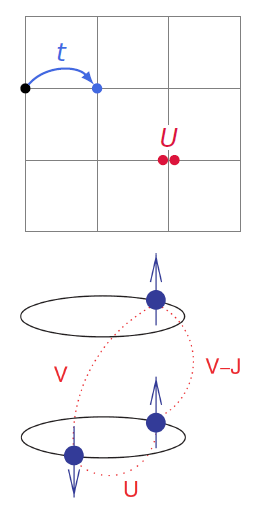
\includegraphics[height=1.35in,width=0.92in,viewport=1 1 240 375,clip]{Figures/LDA_U-1.png}
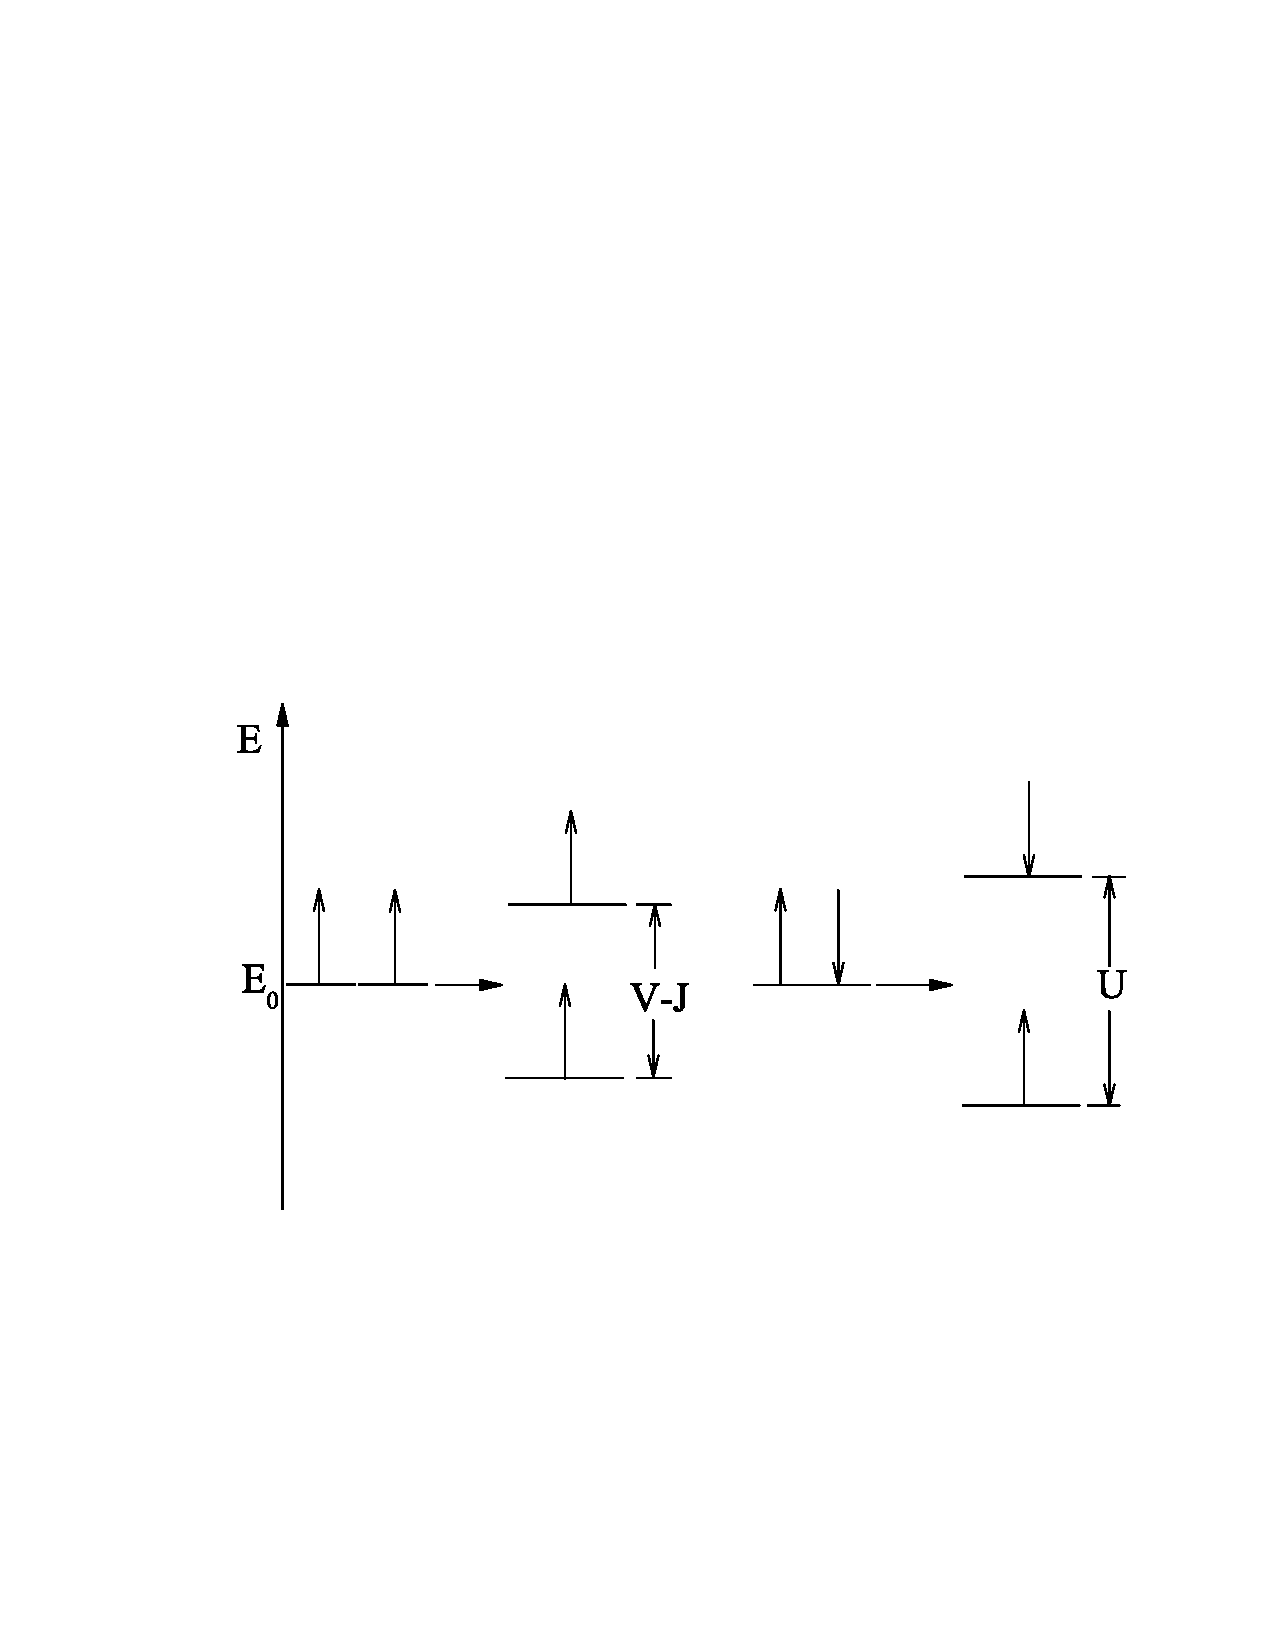
\includegraphics[height=1.35in,width=2.32in,viewport=110 210 545 455,clip]{Figures/LDA_U.pdf}
\caption{\small \textrm{The meaning of $U$, when the Coulomb-interaction of each electron is taken into account.}}%(与文献\cite{EPJB33-47_2003}图1对比)
\label{Tetrahedron_weight}
\end{figure}
}

\frame
{
\frametitle{LDA+$U$近似处理含$d$、$f$\,电子的重元素体系}
对局域的$d$\,或$f$\,电子,用含\textrm{$U$}的模型\textrm{Hamiltonian}考虑$d$-$d$或$f$-$f$间相互作用(定域\textrm{Coulomb}相互作用\textrm{$U$})。%,离域的\textit{s}\,和\textit{p}\,电子的运动用\textrm{LDA}近似描述。
\begin{itemize}
\setlength{\itemsep}{10pt}
	\item \textrm{LDA+$U$}方法最重要的特征:通过参数\textrm{$U$}校正\textrm{LDA}中的电子自相互作用,使单电子能量变化出现不连续。%计算表明LDA+U方法对含有定域强Coulomb相互作用的体系是有效的\upcite{PRB48-16929_1993,JPCS56-1521_1995,EPL36-551_1996}。无论
	\item \textrm{LDA+$U$}方法是平均场近似,对含有近似芯层的局域4$f$\,电子的镧系元素离子还是过渡金属的氧化物(金属的3$d$\,电子与氧原子2$p$\,电子有很强的相互作用)体系都有效。如\textrm{FeSi}和\textrm{LaCaO$_3$}等体系,\textrm{LDA+$U$}能给出有关于金属-绝缘体转变的有用信息。甚至用于含有5$f$\,电子的化合物的研究也取得一定的成功。
\end{itemize}
}

\section{物理性质的计算}
\frame
{
\frametitle{光学性质计算}
\begin{itemize}
\setlength{\itemsep}{10pt}
	\item 半经典方法处理周期性体系的光学性质,用量子力学处理介质,对电磁波仍然采用经典电动力学描写。\upcite{Huang_Han}
	\item 以半导体中的带间垂直跃迁(价带$|v,\vec k\rangle$,导带$|c,\vec k\rangle$)为例讨论固体的能带间跃迁。,晶体中动量为$\vec p$的电子在电磁场(电磁场矢量势为$\vec A$)存在情况下,应用含时微扰理论,准确到$\vec A$的线性项(忽略$\vec A$的平方项)
微扰\textrm{Hamiltonian}为:
\begin{displaymath}
  H^{\prime}=\dfrac{\vec A}c\cdot\vec p
  \label{eq:optic-25}
\end{displaymath}
	\item 频率为$\omega$的平面偏振光,电场和磁场的强度为
\begin{displaymath}
%  \left\{
\begin{aligned}
    \vec E&=-\frac1c\frac{\partial\vec A}{\partial t}\\
    \vec B&=\nabla\times\vec A
  \end{aligned}%\right.
  \label{eq:optic-26}
\end{displaymath}
\end{itemize}
%式中$c$为光速。
}
\frame
{
\frametitle{光学性质的计算}
在含时微扰\textrm{Hamiltonian}作用下,只考虑吸收,跃迁几率为
\begin{displaymath}
  W=2\pi|\langle c,\vec k\,'|H'|v,\vec k\rangle|^2\delta[E_c(\vec k\,')-E_v(\vec k)-\omega]
  \label{eq:optic-27}
\end{displaymath}
$\delta$因子表示跃迁过程的能量守恒关系%,矩阵元$\langle c\vec k|H'|v\vec k\rangle$表示\textrm{Bloch}函数间的积分
。对垂直跃迁,忽略磁场贡献,%矩阵元可以简写成$\dfrac1cA_0\vec e\cdot\vec M_{cv}(\vec k)$,$\vec s$为电磁波矢量势$\vec A_0(=A_0\vec s)$方向的单位矢量。
只有满足能量守恒和动量守恒条件的跃迁才对积分有贡献。%$\displaystyle\int W\dfrac{\textrm{d}\vec k}{(2\pi)^3}$为单位体积、单位时间内吸收能量为$\omega$的光子的总数,系数2是考虑两种自旋态。将式\eqref{eq:optic-27},\eqref{eq:optic-28}代入式\eqref{eq:optic-29},并应用$\dfrac{A_0}c\vec e\cdot\vec M_{cv}(\vec k)$表示矩阵元,得
介质的能量吸收表达式
\begin{displaymath}
  \varepsilon_2(\omega)=2\left(\frac{2\pi}{\omega}\right)^2\sum_{v,c}\int|\vec e\cdot\vec M_{cv}(\vec k)|^2\delta[E_c(\vec k)-E_v(\vec k)-\omega]\frac{\textrm{d}\vec k}{(2\pi)^3}
  \label{eq:optic-32}
\end{displaymath}
即描述能带间跃迁的$\varepsilon(\omega)$微观表达式,是晶体的光学吸收和能带结构之间的基本关系。
对应的$\varepsilon_1$可以根据\textrm{Kramers-Kr\"onig}关系%\eqref{eq:optic-16}
得到
\footnotesize{\begin{displaymath}
  \varepsilon_1(\omega)=1+8\pi\sum_{v,c}\int\frac{|\vec e\cdot\vec M_{cv}(\vec k)|^2}{[E_c(\vec k)-E_v(\vec k)][E_c(\vec k)-E_v(\vec k)]^2-\omega^2}\textrm{d}\vec k\frac2{(2\pi)^3}
  \label{eq:optic-35}
\end{displaymath}}
}
\frame
{
\frametitle{联合态密度(Joint DOS, JDOS)}
定义联合态密度(\textrm{Joint Density of States, JDOS})
\begin{displaymath}
  J_{cv}(\hbar\omega)=\sum_{v,c}\int\delta[E_c(\vec k)-E_v(\vec k)-\omega]\frac{2\textrm{d}\vec k}{(2\pi)^3}
  \label{eq:optic-33}
\end{displaymath}
\footnotesize{令$E_{cv}(\vec k)$\,=\,$E_c(\vec k)-E_v(\vec k)$,因$\textrm{d}\vec k$\,=\,$\dfrac{dE_{cv}(\vec k)}{\nabla_{\vec k}E_{cv}(\vec k)}\textrm{d}S$,故有
\begin{displaymath}
  J_{cv}(\omega)=\frac2{(2\pi)^3}\sum_{v,c}\int\limits_{E_{cv}(\vec k)=\omega}\frac{\textrm{d}S}{\nabla_{\vec k}E_{cv}(\vec k)}
  \label{eq:optic-34}
\end{displaymath}
类似态密度的定义,而$E_{cv}(\vec k)$同时联系着价带和导带,因此称为联合态密度。当矩阵元$\vec M_{cv}(\vec k)$随波矢$\vec k$变化比较小的时候,可以近似地认为$\varepsilon_2(\omega)\!\propto\!J_{cv}(\omega)$。满足$|\nabla_{\vec k}E_{cv}(\vec k)|\!=\!0$的$\vec k$点,是联合态密度$J_{cv}(\omega)$和$\varepsilon_2(\omega)$的奇点(\textrm{Van Hove}奇点或临界点),在这些点,$J_{cv}(\omega)$和$\varepsilon_2(\omega)$%的能谱图将出现典型结构(即
对能量的微商呈现典型的不连续。%联合态密度的奇点有两种情况,即$\nabla_{\vec k}E_c(\vec k)\!=\!\nabla_{\vec k}E_v(\vec k)\!=\!0$和$\nabla_{\vec k}E_c(\vec k)\!=\!\nabla_{\vec k}E_v(\vec k)\!\neq\!0$。将$E_{cv}(\vec k)$在奇点作Taylor级数展开到二级,$$E_{cv}(\vec k)=E_0+a_xk_x^2+a_yk_y^2+a_zk_z^2$$可以看出有四种类型的奇点:
}}

\frame
{
\frametitle{光学函数间的基本关系}
\begin{itemize}
	\item 电磁波在介质中传播,考虑介质的影响,速度为$c/n$,其中$n=\sqrt\varepsilon$为折射率。%类似的,
	\item 考虑介质吸收,折射率$n$用复数$N=n+ik$表示,有$(n(\omega)+ik(\omega))^2=\varepsilon_1(\omega)+i\varepsilon_2(\omega)$,即$N^2=\varepsilon$。由此可得关系式:
\begin{displaymath}
%  \left\{
\begin{aligned}
   \varepsilon_1(\omega)&=n(\omega)^2-k(\omega)^2\\
   \varepsilon_2(\omega)&=2n(\omega)k(\omega)
 \end{aligned}%\right.
  \label{eq:optic-9}
\end{displaymath}
相应地,
\begin{displaymath}
%  \left\{
\begin{aligned}
   n^2&=\frac{\sqrt{\varepsilon_1^2+\varepsilon_2^2}+\varepsilon_1}2\\
   k^2&=\frac{\sqrt{\varepsilon_1^2+\varepsilon_2^2}-\varepsilon_1}2
   \end{aligned}%\right.
  \label{eq:optic-10}
\end{displaymath}
	\item 因此用$\varepsilon_1$,$\varepsilon_2$或用$n$,$k$描述固体的光学性质是等价的。
\end{itemize}
}

\appendix
%------------------------------------------------------------------------Reference----------------------------------------------------------------------------------------------
\begin{thebibliography}{99}
		\frame[allowframebreaks]
{
\frametitle{主要参考文献}
{\tiny
\bibitem{WIEN2k_UG}\textrm{P. Blaha, K. Schwarz, G. Madsen, D. Kvasnicka and J. Luitz. \textit{User's Guide of WIEN2K, An Augmented Plane Wave Plus Local Orbitals Program for Calculating Crystal Properties}. Vienna University of Technology, Inst. of Physical and Theoretical Chemistry, Vienna, Austria (2012)}
\bibitem{PR136-B864_1964}\textrm{P. Hohenberg and W. Kohn \textit{Phys. Rev.} \textbf{136} (1964), B864}
\bibitem{PR140-A1133_1965}\textrm{W. Kohn and L.J. Sham \textit{Phys. Rev.} \textbf{140} (1965), A1133}
\bibitem{Huang_Han}黄昆\:原著、韩汝琦\:改编, \textit{固体物理学}\:高等教育出版社, 北京, 1988
\bibitem{Singh_Book}\textrm{D. J. Singh. \textit{Plane Wave, PseudoPotential and the LAPW method} (Kluwer Academic, Boston,USA, 1994)}
\bibitem{PRB41-7892_1990}\textrm{D. Vanderbilt. \textit{Phys. Rev.} B, \textbf{41} (1990), 7892} 
\bibitem{JPCM6-8245_1994}\textrm{G. Kresse and J. Hafner. J. Phys: \textit{Condens. Matter}, \textbf{6} (1994), 8245}
\bibitem{PRB50-17953_1994}\textrm{P. E. Bl\"ochl. \textit{Phys. Rev.} B, \textbf{50} (1994), 17953}
\bibitem{PRB59-1758_1999}\textrm{G. Kresse and D. Joubert \textit{Phys. Rev.} B, \textbf{59} (1999), 1758}
\bibitem{SSC114-15_2000}\textrm{E. Sj\"ostedt, L. Nordstr\"om and D. J. Singh. \textit{Solid State Commun.}, \textbf{114} (2000), 15}
%\bibitem{VASP_UG}\textrm{G. Kresse, M. Marsman, and J\"urgen Furthm\"uller. \textit{VASP the GUIDE}. Computational Physics, Faculty of Physics, Universit\"at Wien, Austria (2012) \\url http://cms.mpi.univie.ac.at/VASP/}
\bibitem{Comp_Method}\textrm{V. V. Nemoshkalenko and V. N. Antonov. \textit{Computational Methods in Solid State Physics} (Gordon and Breach Science Publisher, Amsterdam, The Netherlands, 1998)}
\bibitem{JMP22-2433_1981}\textrm{M. Weiner. \textit{J. Math. Phys.}, \textbf{22} (1981), 2433}
\bibitem{PRB26-4571_1982}\textrm{M. Weinert, E. Wimmer and A. J. Freeman. \textit{Phys. Rev.} B, \textbf{26} (1982), 4571}
\bibitem{PRB49-16233_1994}\textrm{P. E. Bl\"ochl, O. Jepsen and O. K. Andersen. \textit{Phys. Rev.} B, \textbf{49} (1994), 16233}
\bibitem{PRB44-943_1991}\textrm{V. I. Anisimov, J. Zaanen and O.K. Andersen. \textit{Phys. Rev.} B, \textbf{44} (1991), 943}
\bibitem{PRB48-16929_1993}\textrm{V.I. Anisimov, I.V. Solovyev, M.A. Korotin, M.T. Czyzyk and G.A. Sawatzky. \textit{Phys. Rev.} B, \textbf{48} (1993), 16929}
\nocite{*}																				%
}
}
\end{thebibliography}

%------------------------------------------------------------------------------------------------------------------------------------------------------------------------------%
